\documentclass[a4paper]{article}\usepackage[]{graphicx}\usepackage[]{color}
%% maxwidth is the original width if it is less than linewidth
%% otherwise use linewidth (to make sure the graphics do not exceed the margin)
\makeatletter
\def\maxwidth{ %
  \ifdim\Gin@nat@width>\linewidth
    \linewidth
  \else
    \Gin@nat@width
  \fi
}
\makeatother

\definecolor{fgcolor}{rgb}{0.345, 0.345, 0.345}
\newcommand{\hlnum}[1]{\textcolor[rgb]{0.686,0.059,0.569}{#1}}%
\newcommand{\hlstr}[1]{\textcolor[rgb]{0.192,0.494,0.8}{#1}}%
\newcommand{\hlcom}[1]{\textcolor[rgb]{0.678,0.584,0.686}{\textit{#1}}}%
\newcommand{\hlopt}[1]{\textcolor[rgb]{0,0,0}{#1}}%
\newcommand{\hlstd}[1]{\textcolor[rgb]{0.345,0.345,0.345}{#1}}%
\newcommand{\hlkwa}[1]{\textcolor[rgb]{0.161,0.373,0.58}{\textbf{#1}}}%
\newcommand{\hlkwb}[1]{\textcolor[rgb]{0.69,0.353,0.396}{#1}}%
\newcommand{\hlkwc}[1]{\textcolor[rgb]{0.333,0.667,0.333}{#1}}%
\newcommand{\hlkwd}[1]{\textcolor[rgb]{0.737,0.353,0.396}{\textbf{#1}}}%
\let\hlipl\hlkwb

\usepackage{framed}
\makeatletter
\newenvironment{kframe}{%
 \def\at@end@of@kframe{}%
 \ifinner\ifhmode%
  \def\at@end@of@kframe{\end{minipage}}%
  \begin{minipage}{\columnwidth}%
 \fi\fi%
 \def\FrameCommand##1{\hskip\@totalleftmargin \hskip-\fboxsep
 \colorbox{shadecolor}{##1}\hskip-\fboxsep
     % There is no \\@totalrightmargin, so:
     \hskip-\linewidth \hskip-\@totalleftmargin \hskip\columnwidth}%
 \MakeFramed {\advance\hsize-\width
   \@totalleftmargin\z@ \linewidth\hsize
   \@setminipage}}%
 {\par\unskip\endMakeFramed%
 \at@end@of@kframe}
\makeatother

\definecolor{shadecolor}{rgb}{.97, .97, .97}
\definecolor{messagecolor}{rgb}{0, 0, 0}
\definecolor{warningcolor}{rgb}{1, 0, 1}
\definecolor{errorcolor}{rgb}{1, 0, 0}
\newenvironment{knitrout}{}{} % an empty environment to be redefined in TeX

\usepackage{alltt}

\usepackage{tikz}
\usepackage{pgf}
\usepackage{amsmath}
\newcommand{\gls}[1]{((\textbf{#1}))}
\newcommand{\mw}[1]{\textit{#1}}
\newcommand{\mow}[1]{\textit{#1}}
\IfFileExists{upquote.sty}{\usepackage{upquote}}{}
\begin{document}
\begin{knitrout}
\definecolor{shadecolor}{rgb}{0.969, 0.969, 0.969}\color{fgcolor}\begin{kframe}
\begin{alltt}
\hlkwd{library}\hlstd{(}\hlstr{"tidyverse"}\hlstd{)}
\hlkwd{library}\hlstd{(}\hlstr{"broom"}\hlstd{)}
\hlkwd{library}\hlstd{(}\hlstr{"xtable"}\hlstd{)}
\hlkwd{library}\hlstd{(}\hlstr{"MASS"}\hlstd{)}
\hlkwd{library}\hlstd{(}\hlstr{"ggdendro"}\hlstd{)}
\hlkwd{library}\hlstd{(}\hlstr{"corrplot"}\hlstd{)}
\hlkwd{library}\hlstd{(}\hlstr{"eulerr"}\hlstd{)}
\hlkwd{library}\hlstd{(}\hlstr{"tikzDevice"}\hlstd{)}
\hlkwd{library}\hlstd{(}\hlstr{"knitr"}\hlstd{)}
\hlcom{###THEMES}
\hlkwd{theme_set}\hlstd{(}\hlkwd{theme_bw}\hlstd{())}
\hlstd{scale_colour_discrete} \hlkwb{<-} \hlstd{scale_colour_grey}
\hlstd{scale_fill_discrete} \hlkwb{<-} \hlstd{scale_fill_grey}

\hlcom{###CHUNK OPTIONS}
\hlstd{opts_chunk}\hlopt{$}\hlkwd{set}\hlstd{(}\hlkwc{dev}\hlstd{=}\hlstr{'tikz'}\hlstd{,}
               \hlkwc{external}\hlstd{=}\hlnum{FALSE}\hlstd{,}
               \hlkwc{fig.width}\hlstd{=}\hlnum{5}\hlstd{,}
               \hlkwc{fig.height}\hlstd{=}\hlnum{3.5}\hlstd{)}

\hlcom{###TIKZDEVICE OPTIONS}
\hlkwd{tikz}\hlstd{(}\hlstr{"fontsize-normal.tikz"}\hlstd{)}
\end{alltt}
\end{kframe}
\end{knitrout}

\begin{knitrout}
\definecolor{shadecolor}{rgb}{0.969, 0.969, 0.969}\begin{kframe}
\begin{alltt}
\hlcom{#df.dewi <- read.csv(file="./data/lentypedewi2.csv")}
\hlstd{df.dewi.c} \hlkwb{<-} \hlkwd{read.csv}\hlstd{(}\hlkwc{file}\hlstd{=}\hlstr{"./data/lentypedewi.csv"}\hlstd{)}
\hlstd{glsnames} \hlkwb{<-} \hlkwd{c}\hlstd{(}\hlstr{"\textbackslash{}\textbackslash{}gls\{j119\}"}\hlstd{,}\hlstr{"\textbackslash{}\textbackslash{}gls\{ll27\}"}\hlstd{,}\hlstr{"\textbackslash{}\textbackslash{}gls\{ctd22\}"}\hlstd{)}
\hlkwd{colnames}\hlstd{(df.dewi.c)[}\hlnum{5}\hlopt{:}\hlnum{7}\hlstd{]} \hlkwb{<-} \hlstd{glsnames}
\hlcom{#names(df.dewi) <- gsub("_lenited", "", names(df.dewi))}
\hlstd{df.dewi.c} \hlkwb{<-} \hlstd{df.dewi.c} \hlopt
    \hlkwd{mutate}\hlstd{(}\hlkwc{Lemma} \hlstd{=} \hlkwd{paste}\hlstd{(Word,} \hlstr{" "}\hlstd{, Ll27_p,} \hlstr{"."}\hlstd{, Ll27_l,} \hlkwc{sep}\hlstd{=}\hlstr{""}\hlstd{),}
           \hlkwc{Sum} \hlstd{= (df.dewi.c[,}\hlnum{5}\hlstd{]}\hlopt{+}\hlstd{df.dewi.c[,}\hlnum{6}\hlstd{]}\hlopt{+}\hlstd{df.dewi.c[,}\hlnum{7}\hlstd{]))}
\hlkwd{names}\hlstd{(df.dewi.c)} \hlkwb{<-}
    \hlkwd{gsub}\hlstd{(}\hlstr{"Type.of.lenition"}\hlstd{,} \hlstr{"lenition"}\hlstd{,} \hlkwd{names}\hlstd{(df.dewi.c))}


\hlcom{### Get rid of consonant "c"}
\hlstd{df.dewi} \hlkwb{<-} \hlstd{df.dewi.c} \hlopt \hlkwd{filter}\hlstd{(Initial.consonant} \hlopt{!=} \hlstr{"c"}\hlstd{)}

\hlcom{### Make special free/contact lenition df's}
\hlstd{dewi.free} \hlkwb{<-} \hlstd{df.dewi}  \hlopt
    \hlkwd{filter}\hlstd{(lenition} \hlopt{==} \hlstr{"free"}\hlstd{)}
\hlstd{dewi.cont} \hlkwb{<-} \hlstd{df.dewi}  \hlopt
    \hlkwd{filter}\hlstd{(lenition} \hlopt{==} \hlstr{"contact"}\hlstd{)}
\end{alltt}
\end{kframe}
\end{knitrout}

\begin{knitrout}
\definecolor{shadecolor}{rgb}{0.969, 0.969, 0.969}\begin{kframe}
\begin{alltt}
\hlcom{### Calculate mean rates of representation}
\hlcom{## df.dewi.c[4:7] %>% ## This code is actually more elegant than that below}
\hlcom{##     gather(key=MS,value=Rep, 2:4) %>% }
\hlcom{##     group_by(Initial.consonant, MS) %>% }
\hlcom{##     summarise(mean = format(mean(Rep)*100,digits=3)) %>% }
\hlcom{##     spread(key=Initial.consonant,value=mean)}
\hlstd{firstresults}  \hlkwb{<-} \hlstd{df.dewi.c}  \hlopt
    \hlkwd{gather}\hlstd{(MS,represented,}\hlnum{5}\hlopt{:}\hlnum{7}\hlstd{)}
\hlstd{firstresults} \hlkwb{<-} \hlkwd{aggregate}\hlstd{(firstresults}\hlopt{$}\hlstd{represented,}
          \hlkwc{by}\hlstd{=}\hlkwd{list}\hlstd{(firstresults}\hlopt{$}\hlstd{Initial.consonant,firstresults}\hlopt{$}\hlstd{MS),}
          \hlkwc{FUN}\hlstd{=mean)}\hlopt
    \hlstd{data.frame}  \hlopt
    \hlkwd{mutate}\hlstd{(}\hlkwc{cons}\hlstd{=}\hlkwd{paste}\hlstd{(}\hlstr{"\textbackslash{}\textbackslash{}mw\{"}\hlstd{, Group.1,} \hlstr{"\}"}\hlstd{,} \hlkwc{sep}\hlstd{=}\hlstr{""}\hlstd{),}
           \hlkwc{perc}\hlstd{=}\hlkwd{format}\hlstd{(x}\hlopt{*}\hlnum{100}\hlstd{,}\hlkwc{digits}\hlstd{=}\hlnum{3}\hlstd{),}
           \hlkwc{colcons}\hlstd{=}\hlkwd{paste}\hlstd{(}\hlstr{"\textbackslash{}\textbackslash{}tch\{"}\hlstd{, cons,} \hlstr{"\}"}\hlstd{,} \hlkwc{sep}\hlstd{=}\hlstr{""}\hlstd{))}
\hlstd{firstresults}
\end{alltt}
\begin{verbatim}
##   Group.1      Group.2         x    cons  perc        colcons
## 1       c \\gls{ctd22} 1.0000000 \\mw{c} 100.0 \\tch{\\mw{c}}
## 2       p \\gls{ctd22} 0.8133333 \\mw{p}  81.3 \\tch{\\mw{p}}
## 3       t \\gls{ctd22} 0.9024390 \\mw{t}  90.2 \\tch{\\mw{t}}
## 4       c  \\gls{j119} 1.0000000 \\mw{c} 100.0 \\tch{\\mw{c}}
## 5       p  \\gls{j119} 0.6800000 \\mw{p}  68.0 \\tch{\\mw{p}}
## 6       t  \\gls{j119} 0.6585366 \\mw{t}  65.9 \\tch{\\mw{t}}
## 7       c  \\gls{ll27} 1.0000000 \\mw{c} 100.0 \\tch{\\mw{c}}
## 8       p  \\gls{ll27} 0.8933333 \\mw{p}  89.3 \\tch{\\mw{p}}
## 9       t  \\gls{ll27} 0.8536585 \\mw{t}  85.4 \\tch{\\mw{t}}
\end{verbatim}
\begin{alltt}
\hlcom{### Get these rates in a LaTeX table}
\hlstd{df.results} \hlkwb{<-} \hlstd{firstresults[,}\hlkwd{c}\hlstd{(}\hlnum{2}\hlstd{,}\hlnum{5}\hlstd{,}\hlnum{6}\hlstd{)]} \hlopt
    \hlkwd{spread}\hlstd{(colcons,perc)} \hlopt
    \hlkwd{rename}\hlstd{(}\hlstr{"\textbackslash{}\textbackslash{}tch\{MS\}"} \hlstd{= Group.2)}
\hlstd{df.results} \hlkwb{<-} \hlstd{df.results[,}\hlkwd{c}\hlstd{(}\hlnum{1}\hlstd{,}\hlnum{3}\hlstd{,}\hlnum{4}\hlstd{,}\hlnum{2}\hlstd{)]}
\hlstd{latex.results} \hlkwb{<-} \hlkwd{paste}\hlstd{(}
    \hlstr{"\textbackslash{}\textbackslash{}begin\{tabular\}\{lddd\}\textbackslash{}n\textbackslash{}\textbackslash{}toprule\textbackslash{}n"}\hlstd{,} \hlkwd{colnames}\hlstd{(df.results[}\hlnum{1}\hlstd{]),}
    \hlstr{" & "}\hlstd{,} \hlkwd{colnames}\hlstd{(df.results[}\hlnum{2}\hlstd{]),} \hlstr{" & "}\hlstd{,} \hlkwd{colnames}\hlstd{(df.results[}\hlnum{3}\hlstd{]),}
    \hlstr{" & "}\hlstd{,} \hlkwd{colnames}\hlstd{(df.results[}\hlnum{4}\hlstd{]),} \hlstr{" \textbackslash{}\textbackslash{}\textbackslash{}\textbackslash{} \textbackslash{}\textbackslash{}midrule\textbackslash{}n"}\hlstd{,}
    \hlstd{df.results[}\hlnum{1}\hlstd{,}\hlnum{1}\hlstd{],} \hlstr{" & "}\hlstd{, df.results[}\hlnum{1}\hlstd{,}\hlnum{2}\hlstd{],} \hlstr{" & "}\hlstd{, df.results[}\hlnum{1}\hlstd{,}\hlnum{3}\hlstd{],}
    \hlstr{" & "}\hlstd{, df.results[}\hlnum{1}\hlstd{,}\hlnum{4}\hlstd{],} \hlstr{" \textbackslash{}\textbackslash{}\textbackslash{}\textbackslash{}\textbackslash{}n"}\hlstd{, df.results[}\hlnum{2}\hlstd{,}\hlnum{1}\hlstd{],} \hlstr{" & "}\hlstd{,}
    \hlstd{df.results[}\hlnum{2}\hlstd{,}\hlnum{2}\hlstd{],} \hlstr{" & "}\hlstd{, df.results[}\hlnum{2}\hlstd{,}\hlnum{3}\hlstd{],} \hlstr{" & "}\hlstd{, df.results[}\hlnum{2}\hlstd{,}\hlnum{4}\hlstd{],}
    \hlstr{" \textbackslash{}\textbackslash{}\textbackslash{}\textbackslash{}\textbackslash{}n"}\hlstd{, df.results[}\hlnum{3}\hlstd{,}\hlnum{1}\hlstd{],} \hlstr{" & "}\hlstd{, df.results[}\hlnum{3}\hlstd{,}\hlnum{2}\hlstd{],} \hlstr{" & "}\hlstd{,}
    \hlstd{df.results[}\hlnum{3}\hlstd{,}\hlnum{3}\hlstd{],} \hlstr{" & "}\hlstd{,     df.results[}\hlnum{3}\hlstd{,}\hlnum{4}\hlstd{],}
    \hlstr{" \textbackslash{}\textbackslash{}\textbackslash{}\textbackslash{} \textbackslash{}\textbackslash{}bottomrule\textbackslash{}n\textbackslash{}\textbackslash{}end\{tabular\}\textbackslash{}n"}\hlstd{,} \hlkwc{sep}\hlstd{=}\hlstr{""}\hlstd{)}
\hlkwd{cat}\hlstd{(latex.results,}\hlkwc{file}\hlstd{=}\hlstr{"figure/dewifirstresults.tex"}\hlstd{)}

\hlcom{### Visualise them with a bar plot}
\hlkwd{ggplot}\hlstd{(firstresults,}\hlkwd{aes}\hlstd{(}\hlkwc{x}\hlstd{=} \hlkwd{c}\hlstd{(Group.2),}\hlkwc{y}\hlstd{=}\hlkwd{as.numeric}\hlstd{(perc),}\hlkwc{fill}\hlstd{=cons))}\hlopt{+}
    \hlkwd{geom_col}\hlstd{(}\hlkwc{position}\hlstd{=}\hlstr{"dodge"}\hlstd{,}\hlkwc{color}\hlstd{=}\hlstr{"black"}\hlstd{)}\hlopt{+}
    \hlkwd{labs}\hlstd{(}\hlkwc{x}\hlstd{=}\hlstr{""}\hlstd{,}\hlkwc{y}\hlstd{=}\hlstr{"lenition represented (\textbackslash{}\textbackslash{}%)"}\hlstd{)}\hlopt{+}
    \hlkwd{guides}\hlstd{(}\hlkwc{fill} \hlstd{=} \hlkwd{guide_legend}\hlstd{(}\hlkwc{title} \hlstd{=} \hlstr{"consonant"}\hlstd{))}
\end{alltt}
\end{kframe}
% Created by tikzDevice version 0.11 on 2018-12-11 10:42:14
% !TEX encoding = UTF-8 Unicode
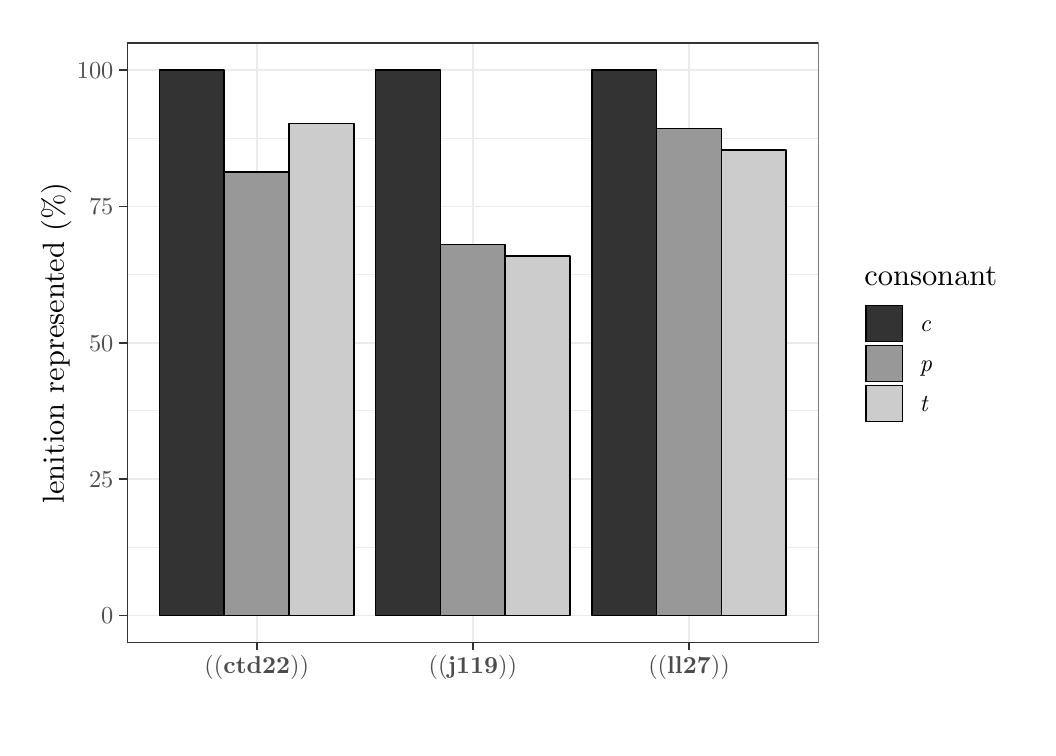
\begin{tikzpicture}[x=1pt,y=1pt]
\definecolor{fillColor}{RGB}{255,255,255}
\path[use as bounding box,fill=fillColor,fill opacity=0.00] (0,0) rectangle (361.35,252.94);
\begin{scope}
\path[clip] (  0.00,  0.00) rectangle (361.35,252.94);
\definecolor{drawColor}{RGB}{255,255,255}
\definecolor{fillColor}{RGB}{255,255,255}

\path[draw=drawColor,line width= 0.6pt,line join=round,line cap=round,fill=fillColor] (  0.00,  0.00) rectangle (361.35,252.94);
\end{scope}
\begin{scope}
\path[clip] ( 35.92, 30.72) rectangle (285.83,247.45);
\definecolor{fillColor}{RGB}{255,255,255}

\path[fill=fillColor] ( 35.92, 30.72) rectangle (285.83,247.45);
\definecolor{drawColor}{gray}{0.92}

\path[draw=drawColor,line width= 0.3pt,line join=round] ( 35.92, 65.20) --
	(285.83, 65.20);

\path[draw=drawColor,line width= 0.3pt,line join=round] ( 35.92,114.46) --
	(285.83,114.46);

\path[draw=drawColor,line width= 0.3pt,line join=round] ( 35.92,163.71) --
	(285.83,163.71);

\path[draw=drawColor,line width= 0.3pt,line join=round] ( 35.92,212.97) --
	(285.83,212.97);

\path[draw=drawColor,line width= 0.6pt,line join=round] ( 35.92, 40.58) --
	(285.83, 40.58);

\path[draw=drawColor,line width= 0.6pt,line join=round] ( 35.92, 89.83) --
	(285.83, 89.83);

\path[draw=drawColor,line width= 0.6pt,line join=round] ( 35.92,139.08) --
	(285.83,139.08);

\path[draw=drawColor,line width= 0.6pt,line join=round] ( 35.92,188.34) --
	(285.83,188.34);

\path[draw=drawColor,line width= 0.6pt,line join=round] ( 35.92,237.59) --
	(285.83,237.59);

\path[draw=drawColor,line width= 0.6pt,line join=round] ( 82.78, 30.72) --
	( 82.78,247.45);

\path[draw=drawColor,line width= 0.6pt,line join=round] (160.87, 30.72) --
	(160.87,247.45);

\path[draw=drawColor,line width= 0.6pt,line join=round] (238.97, 30.72) --
	(238.97,247.45);
\definecolor{drawColor}{RGB}{0,0,0}
\definecolor{fillColor}{gray}{0.80}

\path[draw=drawColor,line width= 0.6pt,line join=round,fill=fillColor] ( 94.49, 40.58) rectangle (117.92,218.29);
\definecolor{fillColor}{RGB}{152,152,152}

\path[draw=drawColor,line width= 0.6pt,line join=round,fill=fillColor] ( 71.06, 40.58) rectangle ( 94.49,200.75);
\definecolor{fillColor}{gray}{0.20}

\path[draw=drawColor,line width= 0.6pt,line join=round,fill=fillColor] ( 47.63, 40.58) rectangle ( 71.06,237.59);
\definecolor{fillColor}{gray}{0.80}

\path[draw=drawColor,line width= 0.6pt,line join=round,fill=fillColor] (172.59, 40.58) rectangle (196.02,170.41);
\definecolor{fillColor}{RGB}{152,152,152}

\path[draw=drawColor,line width= 0.6pt,line join=round,fill=fillColor] (149.16, 40.58) rectangle (172.59,174.55);
\definecolor{fillColor}{gray}{0.20}

\path[draw=drawColor,line width= 0.6pt,line join=round,fill=fillColor] (125.73, 40.58) rectangle (149.16,237.59);
\definecolor{fillColor}{gray}{0.80}

\path[draw=drawColor,line width= 0.6pt,line join=round,fill=fillColor] (250.68, 40.58) rectangle (274.11,208.83);
\definecolor{fillColor}{RGB}{152,152,152}

\path[draw=drawColor,line width= 0.6pt,line join=round,fill=fillColor] (227.26, 40.58) rectangle (250.68,216.51);
\definecolor{fillColor}{gray}{0.20}

\path[draw=drawColor,line width= 0.6pt,line join=round,fill=fillColor] (203.83, 40.58) rectangle (227.26,237.59);
\definecolor{drawColor}{gray}{0.20}

\path[draw=drawColor,line width= 0.6pt,line join=round,line cap=round] ( 35.92, 30.72) rectangle (285.83,247.45);
\end{scope}
\begin{scope}
\path[clip] (  0.00,  0.00) rectangle (361.35,252.94);
\definecolor{drawColor}{gray}{0.30}

\node[text=drawColor,anchor=base east,inner sep=0pt, outer sep=0pt, scale=  0.88] at ( 30.97, 37.55) {0};

\node[text=drawColor,anchor=base east,inner sep=0pt, outer sep=0pt, scale=  0.88] at ( 30.97, 86.80) {25};

\node[text=drawColor,anchor=base east,inner sep=0pt, outer sep=0pt, scale=  0.88] at ( 30.97,136.05) {50};

\node[text=drawColor,anchor=base east,inner sep=0pt, outer sep=0pt, scale=  0.88] at ( 30.97,185.31) {75};

\node[text=drawColor,anchor=base east,inner sep=0pt, outer sep=0pt, scale=  0.88] at ( 30.97,234.56) {100};
\end{scope}
\begin{scope}
\path[clip] (  0.00,  0.00) rectangle (361.35,252.94);
\definecolor{drawColor}{gray}{0.20}

\path[draw=drawColor,line width= 0.6pt,line join=round] ( 33.17, 40.58) --
	( 35.92, 40.58);

\path[draw=drawColor,line width= 0.6pt,line join=round] ( 33.17, 89.83) --
	( 35.92, 89.83);

\path[draw=drawColor,line width= 0.6pt,line join=round] ( 33.17,139.08) --
	( 35.92,139.08);

\path[draw=drawColor,line width= 0.6pt,line join=round] ( 33.17,188.34) --
	( 35.92,188.34);

\path[draw=drawColor,line width= 0.6pt,line join=round] ( 33.17,237.59) --
	( 35.92,237.59);
\end{scope}
\begin{scope}
\path[clip] (  0.00,  0.00) rectangle (361.35,252.94);
\definecolor{drawColor}{gray}{0.20}

\path[draw=drawColor,line width= 0.6pt,line join=round] ( 82.78, 27.97) --
	( 82.78, 30.72);

\path[draw=drawColor,line width= 0.6pt,line join=round] (160.87, 27.97) --
	(160.87, 30.72);

\path[draw=drawColor,line width= 0.6pt,line join=round] (238.97, 27.97) --
	(238.97, 30.72);
\end{scope}
\begin{scope}
\path[clip] (  0.00,  0.00) rectangle (361.35,252.94);
\definecolor{drawColor}{gray}{0.30}

\node[text=drawColor,anchor=base,inner sep=0pt, outer sep=0pt, scale=  0.88] at ( 82.78, 19.71) {\gls{ctd22}};

\node[text=drawColor,anchor=base,inner sep=0pt, outer sep=0pt, scale=  0.88] at (160.87, 19.71) {\gls{j119}};

\node[text=drawColor,anchor=base,inner sep=0pt, outer sep=0pt, scale=  0.88] at (238.97, 19.71) {\gls{ll27}};
\end{scope}
\begin{scope}
\path[clip] (  0.00,  0.00) rectangle (361.35,252.94);
\definecolor{drawColor}{RGB}{0,0,0}

\node[text=drawColor,rotate= 90.00,anchor=base,inner sep=0pt, outer sep=0pt, scale=  1.10] at ( 13.08,139.08) {lenition represented (\%)};
\end{scope}
\begin{scope}
\path[clip] (  0.00,  0.00) rectangle (361.35,252.94);
\definecolor{fillColor}{RGB}{255,255,255}

\path[fill=fillColor] (296.83,104.39) rectangle (355.85,173.78);
\end{scope}
\begin{scope}
\path[clip] (  0.00,  0.00) rectangle (361.35,252.94);
\definecolor{drawColor}{RGB}{0,0,0}

\node[text=drawColor,anchor=base west,inner sep=0pt, outer sep=0pt, scale=  1.10] at (302.33,159.73) {consonant};
\end{scope}
\begin{scope}
\path[clip] (  0.00,  0.00) rectangle (361.35,252.94);
\definecolor{fillColor}{RGB}{255,255,255}

\path[fill=fillColor] (302.33,138.80) rectangle (316.78,153.26);
\end{scope}
\begin{scope}
\path[clip] (  0.00,  0.00) rectangle (361.35,252.94);
\definecolor{drawColor}{RGB}{0,0,0}
\definecolor{fillColor}{gray}{0.20}

\path[draw=drawColor,line width= 0.6pt,line cap=round,fill=fillColor] (303.04,139.51) rectangle (316.07,152.54);
\end{scope}
\begin{scope}
\path[clip] (  0.00,  0.00) rectangle (361.35,252.94);
\definecolor{fillColor}{RGB}{255,255,255}

\path[fill=fillColor] (302.33,124.35) rectangle (316.78,138.80);
\end{scope}
\begin{scope}
\path[clip] (  0.00,  0.00) rectangle (361.35,252.94);
\definecolor{drawColor}{RGB}{0,0,0}
\definecolor{fillColor}{RGB}{152,152,152}

\path[draw=drawColor,line width= 0.6pt,line cap=round,fill=fillColor] (303.04,125.06) rectangle (316.07,138.09);
\end{scope}
\begin{scope}
\path[clip] (  0.00,  0.00) rectangle (361.35,252.94);
\definecolor{fillColor}{RGB}{255,255,255}

\path[fill=fillColor] (302.33,109.89) rectangle (316.78,124.35);
\end{scope}
\begin{scope}
\path[clip] (  0.00,  0.00) rectangle (361.35,252.94);
\definecolor{drawColor}{RGB}{0,0,0}
\definecolor{fillColor}{gray}{0.80}

\path[draw=drawColor,line width= 0.6pt,line cap=round,fill=fillColor] (303.04,110.61) rectangle (316.07,123.64);
\end{scope}
\begin{scope}
\path[clip] (  0.00,  0.00) rectangle (361.35,252.94);
\definecolor{drawColor}{RGB}{0,0,0}

\node[text=drawColor,anchor=base west,inner sep=0pt, outer sep=0pt, scale=  0.88] at (322.28,143.00) {\mw{c}};
\end{scope}
\begin{scope}
\path[clip] (  0.00,  0.00) rectangle (361.35,252.94);
\definecolor{drawColor}{RGB}{0,0,0}

\node[text=drawColor,anchor=base west,inner sep=0pt, outer sep=0pt, scale=  0.88] at (322.28,128.54) {\mw{p}};
\end{scope}
\begin{scope}
\path[clip] (  0.00,  0.00) rectangle (361.35,252.94);
\definecolor{drawColor}{RGB}{0,0,0}

\node[text=drawColor,anchor=base west,inner sep=0pt, outer sep=0pt, scale=  0.88] at (322.28,114.09) {\mw{t}};
\end{scope}
\end{tikzpicture}

\begin{kframe}\begin{alltt}
\hlcom{### Alternative with stacked bars; NB unweighed for rel. freq of p t c}
\hlkwd{ggplot}\hlstd{(firstresults,}\hlkwd{aes}\hlstd{(}\hlkwc{x}\hlstd{=} \hlkwd{c}\hlstd{(Group.2),}\hlkwc{y}\hlstd{=}\hlkwd{as.numeric}\hlstd{(perc)}\hlopt{/}\hlnum{3}\hlstd{,}\hlkwc{fill}\hlstd{=cons))}\hlopt{+}
    \hlkwd{geom_col}\hlstd{(}\hlkwc{position}\hlstd{=}\hlstr{"stack"}\hlstd{,}\hlkwc{color}\hlstd{=}\hlstr{"black"}\hlstd{)}\hlopt{+}
    \hlkwd{labs}\hlstd{(}\hlkwc{x}\hlstd{=}\hlstr{""}\hlstd{,}\hlkwc{y}\hlstd{=}\hlstr{"lenition represented (\textbackslash{}\textbackslash{}%)"}\hlstd{)}\hlopt{+}
    \hlkwd{ylim}\hlstd{(}\hlnum{0}\hlstd{,}\hlnum{100}\hlstd{)}\hlopt{+}
    \hlkwd{guides}\hlstd{(}\hlkwc{fill} \hlstd{=} \hlkwd{guide_legend}\hlstd{(}\hlkwc{title} \hlstd{=} \hlstr{"consonant"}\hlstd{))}
\end{alltt}
\end{kframe}
% Created by tikzDevice version 0.11 on 2018-12-11 10:42:15
% !TEX encoding = UTF-8 Unicode
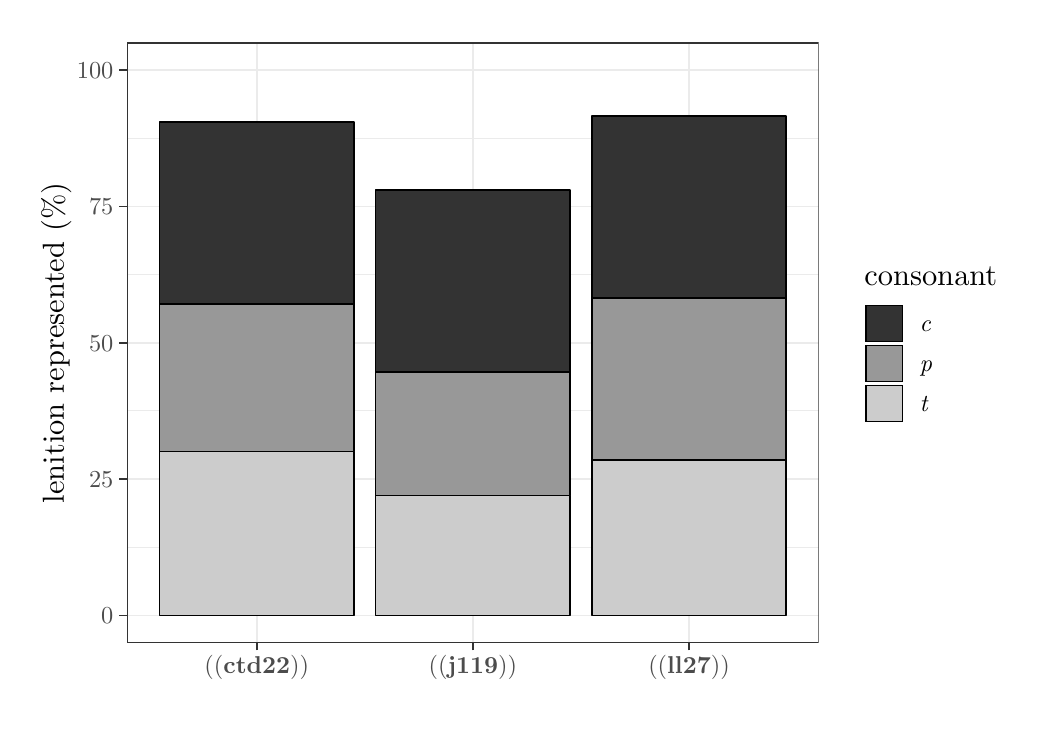
\begin{tikzpicture}[x=1pt,y=1pt]
\definecolor{fillColor}{RGB}{255,255,255}
\path[use as bounding box,fill=fillColor,fill opacity=0.00] (0,0) rectangle (361.35,252.94);
\begin{scope}
\path[clip] (  0.00,  0.00) rectangle (361.35,252.94);
\definecolor{drawColor}{RGB}{255,255,255}
\definecolor{fillColor}{RGB}{255,255,255}

\path[draw=drawColor,line width= 0.6pt,line join=round,line cap=round,fill=fillColor] (  0.00,  0.00) rectangle (361.35,252.94);
\end{scope}
\begin{scope}
\path[clip] ( 35.92, 30.72) rectangle (285.83,247.45);
\definecolor{fillColor}{RGB}{255,255,255}

\path[fill=fillColor] ( 35.92, 30.72) rectangle (285.83,247.45);
\definecolor{drawColor}{gray}{0.92}

\path[draw=drawColor,line width= 0.3pt,line join=round] ( 35.92, 65.20) --
	(285.83, 65.20);

\path[draw=drawColor,line width= 0.3pt,line join=round] ( 35.92,114.46) --
	(285.83,114.46);

\path[draw=drawColor,line width= 0.3pt,line join=round] ( 35.92,163.71) --
	(285.83,163.71);

\path[draw=drawColor,line width= 0.3pt,line join=round] ( 35.92,212.97) --
	(285.83,212.97);

\path[draw=drawColor,line width= 0.6pt,line join=round] ( 35.92, 40.58) --
	(285.83, 40.58);

\path[draw=drawColor,line width= 0.6pt,line join=round] ( 35.92, 89.83) --
	(285.83, 89.83);

\path[draw=drawColor,line width= 0.6pt,line join=round] ( 35.92,139.08) --
	(285.83,139.08);

\path[draw=drawColor,line width= 0.6pt,line join=round] ( 35.92,188.34) --
	(285.83,188.34);

\path[draw=drawColor,line width= 0.6pt,line join=round] ( 35.92,237.59) --
	(285.83,237.59);

\path[draw=drawColor,line width= 0.6pt,line join=round] ( 82.78, 30.72) --
	( 82.78,247.45);

\path[draw=drawColor,line width= 0.6pt,line join=round] (160.87, 30.72) --
	(160.87,247.45);

\path[draw=drawColor,line width= 0.6pt,line join=round] (238.97, 30.72) --
	(238.97,247.45);
\definecolor{drawColor}{RGB}{0,0,0}
\definecolor{fillColor}{gray}{0.80}

\path[draw=drawColor,line width= 0.6pt,line join=round,fill=fillColor] ( 47.63, 40.58) rectangle (117.92, 99.81);
\definecolor{fillColor}{RGB}{152,152,152}

\path[draw=drawColor,line width= 0.6pt,line join=round,fill=fillColor] ( 47.63, 99.81) rectangle (117.92,153.20);
\definecolor{fillColor}{gray}{0.20}

\path[draw=drawColor,line width= 0.6pt,line join=round,fill=fillColor] ( 47.63,153.20) rectangle (117.92,218.88);
\definecolor{fillColor}{gray}{0.80}

\path[draw=drawColor,line width= 0.6pt,line join=round,fill=fillColor] (125.73, 40.58) rectangle (196.02, 83.85);
\definecolor{fillColor}{RGB}{152,152,152}

\path[draw=drawColor,line width= 0.6pt,line join=round,fill=fillColor] (125.73, 83.85) rectangle (196.02,128.51);
\definecolor{fillColor}{gray}{0.20}

\path[draw=drawColor,line width= 0.6pt,line join=round,fill=fillColor] (125.73,128.51) rectangle (196.02,194.18);
\definecolor{fillColor}{gray}{0.80}

\path[draw=drawColor,line width= 0.6pt,line join=round,fill=fillColor] (203.83, 40.58) rectangle (274.11, 96.66);
\definecolor{fillColor}{RGB}{152,152,152}

\path[draw=drawColor,line width= 0.6pt,line join=round,fill=fillColor] (203.83, 96.66) rectangle (274.11,155.31);
\definecolor{fillColor}{gray}{0.20}

\path[draw=drawColor,line width= 0.6pt,line join=round,fill=fillColor] (203.83,155.31) rectangle (274.11,220.98);
\definecolor{drawColor}{gray}{0.20}

\path[draw=drawColor,line width= 0.6pt,line join=round,line cap=round] ( 35.92, 30.72) rectangle (285.83,247.45);
\end{scope}
\begin{scope}
\path[clip] (  0.00,  0.00) rectangle (361.35,252.94);
\definecolor{drawColor}{gray}{0.30}

\node[text=drawColor,anchor=base east,inner sep=0pt, outer sep=0pt, scale=  0.88] at ( 30.97, 37.55) {0};

\node[text=drawColor,anchor=base east,inner sep=0pt, outer sep=0pt, scale=  0.88] at ( 30.97, 86.80) {25};

\node[text=drawColor,anchor=base east,inner sep=0pt, outer sep=0pt, scale=  0.88] at ( 30.97,136.05) {50};

\node[text=drawColor,anchor=base east,inner sep=0pt, outer sep=0pt, scale=  0.88] at ( 30.97,185.31) {75};

\node[text=drawColor,anchor=base east,inner sep=0pt, outer sep=0pt, scale=  0.88] at ( 30.97,234.56) {100};
\end{scope}
\begin{scope}
\path[clip] (  0.00,  0.00) rectangle (361.35,252.94);
\definecolor{drawColor}{gray}{0.20}

\path[draw=drawColor,line width= 0.6pt,line join=round] ( 33.17, 40.58) --
	( 35.92, 40.58);

\path[draw=drawColor,line width= 0.6pt,line join=round] ( 33.17, 89.83) --
	( 35.92, 89.83);

\path[draw=drawColor,line width= 0.6pt,line join=round] ( 33.17,139.08) --
	( 35.92,139.08);

\path[draw=drawColor,line width= 0.6pt,line join=round] ( 33.17,188.34) --
	( 35.92,188.34);

\path[draw=drawColor,line width= 0.6pt,line join=round] ( 33.17,237.59) --
	( 35.92,237.59);
\end{scope}
\begin{scope}
\path[clip] (  0.00,  0.00) rectangle (361.35,252.94);
\definecolor{drawColor}{gray}{0.20}

\path[draw=drawColor,line width= 0.6pt,line join=round] ( 82.78, 27.97) --
	( 82.78, 30.72);

\path[draw=drawColor,line width= 0.6pt,line join=round] (160.87, 27.97) --
	(160.87, 30.72);

\path[draw=drawColor,line width= 0.6pt,line join=round] (238.97, 27.97) --
	(238.97, 30.72);
\end{scope}
\begin{scope}
\path[clip] (  0.00,  0.00) rectangle (361.35,252.94);
\definecolor{drawColor}{gray}{0.30}

\node[text=drawColor,anchor=base,inner sep=0pt, outer sep=0pt, scale=  0.88] at ( 82.78, 19.71) {\gls{ctd22}};

\node[text=drawColor,anchor=base,inner sep=0pt, outer sep=0pt, scale=  0.88] at (160.87, 19.71) {\gls{j119}};

\node[text=drawColor,anchor=base,inner sep=0pt, outer sep=0pt, scale=  0.88] at (238.97, 19.71) {\gls{ll27}};
\end{scope}
\begin{scope}
\path[clip] (  0.00,  0.00) rectangle (361.35,252.94);
\definecolor{drawColor}{RGB}{0,0,0}

\node[text=drawColor,rotate= 90.00,anchor=base,inner sep=0pt, outer sep=0pt, scale=  1.10] at ( 13.08,139.08) {lenition represented (\%)};
\end{scope}
\begin{scope}
\path[clip] (  0.00,  0.00) rectangle (361.35,252.94);
\definecolor{fillColor}{RGB}{255,255,255}

\path[fill=fillColor] (296.83,104.39) rectangle (355.85,173.78);
\end{scope}
\begin{scope}
\path[clip] (  0.00,  0.00) rectangle (361.35,252.94);
\definecolor{drawColor}{RGB}{0,0,0}

\node[text=drawColor,anchor=base west,inner sep=0pt, outer sep=0pt, scale=  1.10] at (302.33,159.73) {consonant};
\end{scope}
\begin{scope}
\path[clip] (  0.00,  0.00) rectangle (361.35,252.94);
\definecolor{fillColor}{RGB}{255,255,255}

\path[fill=fillColor] (302.33,138.80) rectangle (316.78,153.26);
\end{scope}
\begin{scope}
\path[clip] (  0.00,  0.00) rectangle (361.35,252.94);
\definecolor{drawColor}{RGB}{0,0,0}
\definecolor{fillColor}{gray}{0.20}

\path[draw=drawColor,line width= 0.6pt,line cap=round,fill=fillColor] (303.04,139.51) rectangle (316.07,152.54);
\end{scope}
\begin{scope}
\path[clip] (  0.00,  0.00) rectangle (361.35,252.94);
\definecolor{fillColor}{RGB}{255,255,255}

\path[fill=fillColor] (302.33,124.35) rectangle (316.78,138.80);
\end{scope}
\begin{scope}
\path[clip] (  0.00,  0.00) rectangle (361.35,252.94);
\definecolor{drawColor}{RGB}{0,0,0}
\definecolor{fillColor}{RGB}{152,152,152}

\path[draw=drawColor,line width= 0.6pt,line cap=round,fill=fillColor] (303.04,125.06) rectangle (316.07,138.09);
\end{scope}
\begin{scope}
\path[clip] (  0.00,  0.00) rectangle (361.35,252.94);
\definecolor{fillColor}{RGB}{255,255,255}

\path[fill=fillColor] (302.33,109.89) rectangle (316.78,124.35);
\end{scope}
\begin{scope}
\path[clip] (  0.00,  0.00) rectangle (361.35,252.94);
\definecolor{drawColor}{RGB}{0,0,0}
\definecolor{fillColor}{gray}{0.80}

\path[draw=drawColor,line width= 0.6pt,line cap=round,fill=fillColor] (303.04,110.61) rectangle (316.07,123.64);
\end{scope}
\begin{scope}
\path[clip] (  0.00,  0.00) rectangle (361.35,252.94);
\definecolor{drawColor}{RGB}{0,0,0}

\node[text=drawColor,anchor=base west,inner sep=0pt, outer sep=0pt, scale=  0.88] at (322.28,143.00) {\mw{c}};
\end{scope}
\begin{scope}
\path[clip] (  0.00,  0.00) rectangle (361.35,252.94);
\definecolor{drawColor}{RGB}{0,0,0}

\node[text=drawColor,anchor=base west,inner sep=0pt, outer sep=0pt, scale=  0.88] at (322.28,128.54) {\mw{p}};
\end{scope}
\begin{scope}
\path[clip] (  0.00,  0.00) rectangle (361.35,252.94);
\definecolor{drawColor}{RGB}{0,0,0}

\node[text=drawColor,anchor=base west,inner sep=0pt, outer sep=0pt, scale=  0.88] at (322.28,114.09) {\mw{t}};
\end{scope}
\end{tikzpicture}


\end{knitrout}

\begin{knitrout}
\definecolor{shadecolor}{rgb}{0.969, 0.969, 0.969}\begin{kframe}
\begin{alltt}
\hlcom{### Here we generate the right numbers for the different contingency tables}

\hlcom{### Contingency table for observed values}
\hlstd{obs.ll27ctd22} \hlkwb{<-} \hlstd{df.dewi}  \hlopt
    \hlkwd{summarise}\hlstd{(}
        \hlkwc{AA} \hlstd{=} \hlkwd{nrow}\hlstd{(}\hlkwd{filter}\hlstd{(.,`\textbackslash{}\textbackslash{}gls\{ll27\}`} \hlopt{==} \hlnum{FALSE} \hlopt{&} \hlstd{`\textbackslash{}\textbackslash{}gls\{ctd22\}`} \hlopt{==} \hlnum{FALSE}\hlstd{)),}
        \hlkwc{AI} \hlstd{=} \hlkwd{nrow}\hlstd{(}\hlkwd{filter}\hlstd{(.,`\textbackslash{}\textbackslash{}gls\{ll27\}`} \hlopt{==} \hlnum{FALSE} \hlopt{&} \hlstd{`\textbackslash{}\textbackslash{}gls\{ctd22\}`} \hlopt{==} \hlnum{TRUE}\hlstd{)),}
        \hlkwc{IA} \hlstd{=} \hlkwd{nrow}\hlstd{(}\hlkwd{filter}\hlstd{(.,`\textbackslash{}\textbackslash{}gls\{ll27\}`} \hlopt{==} \hlnum{TRUE} \hlopt{&} \hlstd{`\textbackslash{}\textbackslash{}gls\{ctd22\}`} \hlopt{==} \hlnum{FALSE}\hlstd{)),}
        \hlkwc{II} \hlstd{=} \hlkwd{nrow}\hlstd{(}\hlkwd{filter}\hlstd{(.,`\textbackslash{}\textbackslash{}gls\{ll27\}`} \hlopt{==} \hlnum{TRUE} \hlopt{&} \hlstd{`\textbackslash{}\textbackslash{}gls\{ctd22\}`} \hlopt{==} \hlnum{TRUE}\hlstd{))}
    \hlstd{)} \hlopt \hlstd{as.numeric}  \hlopt \hlkwd{matrix}\hlstd{(}\hlkwc{nrow}\hlstd{=}\hlnum{2}\hlstd{)}

\hlstd{obs.j119ll27} \hlkwb{<-} \hlstd{df.dewi}  \hlopt
    \hlkwd{summarise}\hlstd{(}
        \hlkwc{AA} \hlstd{=} \hlkwd{nrow}\hlstd{(}\hlkwd{filter}\hlstd{(.,`\textbackslash{}\textbackslash{}gls\{j119\}`} \hlopt{==} \hlnum{FALSE} \hlopt{&} \hlstd{`\textbackslash{}\textbackslash{}gls\{ll27\}`} \hlopt{==} \hlnum{FALSE}\hlstd{)),}
        \hlkwc{AI} \hlstd{=} \hlkwd{nrow}\hlstd{(}\hlkwd{filter}\hlstd{(.,`\textbackslash{}\textbackslash{}gls\{j119\}`} \hlopt{==} \hlnum{FALSE} \hlopt{&} \hlstd{`\textbackslash{}\textbackslash{}gls\{ll27\}`} \hlopt{==} \hlnum{TRUE}\hlstd{)),}
        \hlkwc{IA} \hlstd{=} \hlkwd{nrow}\hlstd{(}\hlkwd{filter}\hlstd{(.,`\textbackslash{}\textbackslash{}gls\{j119\}`} \hlopt{==} \hlnum{TRUE} \hlopt{&} \hlstd{`\textbackslash{}\textbackslash{}gls\{ll27\}`} \hlopt{==} \hlnum{FALSE}\hlstd{)),}
        \hlkwc{II} \hlstd{=} \hlkwd{nrow}\hlstd{(}\hlkwd{filter}\hlstd{(.,`\textbackslash{}\textbackslash{}gls\{j119\}`} \hlopt{==} \hlnum{TRUE} \hlopt{&} \hlstd{`\textbackslash{}\textbackslash{}gls\{ll27\}`} \hlopt{==} \hlnum{TRUE}\hlstd{))}
    \hlstd{)} \hlopt \hlstd{as.numeric}  \hlopt \hlkwd{matrix}\hlstd{(}\hlkwc{nrow}\hlstd{=}\hlnum{2}\hlstd{)}

\hlstd{obs.ctd22j119} \hlkwb{<-} \hlstd{df.dewi}  \hlopt
    \hlkwd{summarise}\hlstd{(}
        \hlkwc{AA} \hlstd{=} \hlkwd{nrow}\hlstd{(}\hlkwd{filter}\hlstd{(.,`\textbackslash{}\textbackslash{}gls\{ctd22\}`} \hlopt{==} \hlnum{FALSE} \hlopt{&} \hlstd{`\textbackslash{}\textbackslash{}gls\{j119\}`} \hlopt{==} \hlnum{FALSE}\hlstd{)),}
        \hlkwc{AI} \hlstd{=} \hlkwd{nrow}\hlstd{(}\hlkwd{filter}\hlstd{(.,`\textbackslash{}\textbackslash{}gls\{ctd22\}`} \hlopt{==} \hlnum{FALSE} \hlopt{&} \hlstd{`\textbackslash{}\textbackslash{}gls\{j119\}`} \hlopt{==} \hlnum{TRUE}\hlstd{)),}
        \hlkwc{IA} \hlstd{=} \hlkwd{nrow}\hlstd{(}\hlkwd{filter}\hlstd{(.,`\textbackslash{}\textbackslash{}gls\{ctd22\}`} \hlopt{==} \hlnum{TRUE} \hlopt{&} \hlstd{`\textbackslash{}\textbackslash{}gls\{j119\}`} \hlopt{==} \hlnum{FALSE}\hlstd{)),}
        \hlkwc{II} \hlstd{=} \hlkwd{nrow}\hlstd{(}\hlkwd{filter}\hlstd{(.,`\textbackslash{}\textbackslash{}gls\{ctd22\}`} \hlopt{==} \hlnum{TRUE} \hlopt{&} \hlstd{`\textbackslash{}\textbackslash{}gls\{j119\}`} \hlopt{==} \hlnum{TRUE}\hlstd{))}
    \hlstd{)} \hlopt \hlstd{as.numeric}  \hlopt \hlkwd{matrix}\hlstd{(}\hlkwc{nrow}\hlstd{=}\hlnum{2}\hlstd{)}

\hlcom{### Calculating expected values}
\hlstd{expval} \hlkwb{<-} \hlkwa{function}\hlstd{(}\hlkwc{x}\hlstd{,}\hlkwc{r}\hlstd{,}\hlkwc{c}\hlstd{)\{}\hlkwd{rowSums}\hlstd{(x)[r]}\hlopt{*}\hlkwd{colSums}\hlstd{(x)[c]}\hlopt{/}\hlkwd{sum}\hlstd{(x)\}}
\hlstd{expmat} \hlkwb{<-} \hlkwa{function}\hlstd{(}\hlkwc{x}\hlstd{)\{}
    \hlstd{exp_lst} \hlkwb{<-} \hlkwd{list}\hlstd{()}
    \hlkwa{for} \hlstd{(i} \hlkwa{in} \hlnum{1}\hlopt{:}\hlkwd{ncol}\hlstd{(x))\{exp_lst[[i]]} \hlkwb{<-} \hlkwd{expval}\hlstd{(}\hlkwc{x}\hlstd{=x,}\hlkwc{r}\hlstd{=}\hlnum{1}\hlopt{:}\hlkwd{nrow}\hlstd{(x),}\hlkwc{c}\hlstd{=i)\}}
    \hlkwd{matrix}\hlstd{(}\hlkwd{unlist}\hlstd{(exp_lst),}\hlkwc{nrow}\hlstd{=}\hlkwd{nrow}\hlstd{(x),}\hlkwc{byrow}\hlstd{=}\hlnum{FALSE}\hlstd{)\}}
\hlstd{exp.ll27ctd22} \hlkwb{<-} \hlstd{obs.ll27ctd22}  \hlopt \hlstd{expmat}
\hlstd{exp.j119ll27} \hlkwb{<-} \hlstd{obs.j119ll27}  \hlopt \hlstd{expmat}
\hlstd{exp.ctd22j119} \hlkwb{<-} \hlstd{obs.ctd22j119}  \hlopt \hlstd{expmat}

\hlcom{### Calculating squared residuals}
\hlstd{sqres} \hlkwb{<-} \hlkwa{function}\hlstd{(}\hlkwc{o}\hlstd{,}\hlkwc{e}\hlstd{=}\hlkwd{expmat}\hlstd{(o))\{((o}\hlopt{-}\hlstd{e)}\hlopt{^}\hlnum{2}\hlstd{)}\hlopt{/}\hlstd{e\}}
\hlstd{sqres.ll27ctd22} \hlkwb{<-} \hlstd{obs.ll27ctd22}  \hlopt \hlstd{sqres}
\hlstd{sqres.j119ll27} \hlkwb{<-} \hlstd{obs.j119ll27}  \hlopt \hlstd{sqres}
\hlstd{sqres.ctd22j119} \hlkwb{<-} \hlstd{obs.ctd22j119}  \hlopt \hlstd{sqres}

\hlcom{### Calculating chi-squared score}
\hlstd{chisq.ll27ctd22} \hlkwb{<-} \hlstd{sqres.ll27ctd22}  \hlopt \hlstd{sum}
\hlstd{chisq.j119ll27} \hlkwb{<-} \hlstd{sqres.j119ll27}  \hlopt \hlstd{sum}
\hlstd{chisq.ctd22j119} \hlkwb{<-} \hlstd{sqres.ctd22j119}  \hlopt \hlstd{sum}

\hlstd{cont.table.tot} \hlkwb{<-} \hlkwa{function}\hlstd{(}\hlkwc{d}\hlstd{,}\hlkwc{x}\hlstd{,}\hlkwc{y}\hlstd{)\{}
    \hlkwd{paste}\hlstd{(}\hlstr{"\textbackslash{}\textbackslash{}begin\{tabular\}\{ccddd\}\textbackslash{}n\textbackslash{}\textbackslash{}toprule\textbackslash{}n & & \textbackslash{}\textbackslash{}tchhh\{\textbackslash{}\textbackslash{}gls\{"}\hlstd{,}
          \hlstd{x,}
          \hlstr{"\}\} \textbackslash{}\textbackslash{}\textbackslash{}\textbackslash{}\textbackslash{}n& & \textbackslash{}\textbackslash{}tch\{A\} & \textbackslash{}\textbackslash{}tch\{I\} & \textbackslash{}\textbackslash{}tch\{Total\}\textbackslash{}\textbackslash{}\textbackslash{}\textbackslash{}\textbackslash{}n\textbackslash{}\textbackslash{}multirow\{3\}\{*\}\{\textbackslash{}\textbackslash{}gls\{"}\hlstd{,}
          \hlstd{y,}
          \hlstr{"\}\} & A  & "}\hlstd{,}
          \hlkwd{round}\hlstd{(d[}\hlnum{1}\hlstd{,}\hlnum{1}\hlstd{],}\hlnum{2}\hlstd{),}
          \hlstr{" & "}\hlstd{,}
          \hlkwd{round}\hlstd{(d[}\hlnum{1}\hlstd{,}\hlnum{2}\hlstd{],}\hlnum{2}\hlstd{),}
          \hlstr{" & "}\hlstd{,}
          \hlkwd{round}\hlstd{(}\hlkwd{sum}\hlstd{(d[}\hlnum{1}\hlstd{,}\hlnum{1}\hlopt{:}\hlnum{2}\hlstd{]),}\hlnum{2}\hlstd{),}
          \hlstr{"\textbackslash{}\textbackslash{}\textbackslash{}\textbackslash{}\textbackslash{}n& I & "}\hlstd{,}
          \hlkwd{round}\hlstd{(d[}\hlnum{2}\hlstd{,}\hlnum{1}\hlstd{],}\hlnum{2}\hlstd{),}
          \hlstr{" & "}\hlstd{,}
          \hlkwd{round}\hlstd{(d[}\hlnum{2}\hlstd{,}\hlnum{2}\hlstd{],}\hlnum{2}\hlstd{),}
          \hlstr{" & "}\hlstd{,}
          \hlkwd{round}\hlstd{(}\hlkwd{sum}\hlstd{(d[}\hlnum{2}\hlstd{,}\hlnum{1}\hlopt{:}\hlnum{2}\hlstd{]),}\hlnum{2}\hlstd{),}
          \hlstr{"\textbackslash{}\textbackslash{}\textbackslash{}\textbackslash{}\textbackslash{}n& Total & "}\hlstd{,}
          \hlkwd{round}\hlstd{(}\hlkwd{sum}\hlstd{(d[}\hlnum{1}\hlopt{:}\hlnum{2}\hlstd{,}\hlnum{1}\hlstd{]),}\hlnum{2}\hlstd{),}
          \hlstr{" & "}\hlstd{,}
          \hlkwd{round}\hlstd{(}\hlkwd{sum}\hlstd{(d[}\hlnum{1}\hlopt{:}\hlnum{2}\hlstd{,}\hlnum{2}\hlstd{]),}\hlnum{2}\hlstd{),}
          \hlstr{" & "}\hlstd{,}
          \hlkwd{round}\hlstd{(}\hlkwd{sum}\hlstd{(d),}\hlnum{2}\hlstd{),}
          \hlstr{"\textbackslash{}\textbackslash{}\textbackslash{}\textbackslash{}\textbackslash{}\textbackslash{}bottomrule\textbackslash{}n\textbackslash{}\textbackslash{}end\{tabular\}"}\hlstd{,}
          \hlkwc{sep}\hlstd{=}\hlstr{""}\hlstd{)}
\hlstd{\}}
\hlkwd{cont.table.tot}\hlstd{(}\hlkwc{d}\hlstd{=obs.ll27ctd22,}\hlkwc{x}\hlstd{=}\hlstr{"ll27"}\hlstd{,}\hlkwc{y}\hlstd{=}\hlstr{"ctd22"}\hlstd{)} \hlopt
    \hlkwd{cat}\hlstd{(}\hlkwc{file}\hlstd{=}\hlstr{"figure/obsll27ctd22.tex"}\hlstd{)}
\hlkwd{cont.table.tot}\hlstd{(}\hlkwc{d}\hlstd{=obs.j119ll27,}\hlkwc{x}\hlstd{=}\hlstr{"j119"}\hlstd{,}\hlkwc{y}\hlstd{=}\hlstr{"ll27"}\hlstd{)} \hlopt
    \hlkwd{cat}\hlstd{(}\hlkwc{file}\hlstd{=}\hlstr{"figure/obsj119ll27.tex"}\hlstd{)}
\hlkwd{cont.table.tot}\hlstd{(}\hlkwc{d}\hlstd{=obs.ctd22j119,}\hlkwc{x}\hlstd{=}\hlstr{"ctd22"}\hlstd{,}\hlkwc{y}\hlstd{=}\hlstr{"j119"}\hlstd{)} \hlopt
    \hlkwd{cat}\hlstd{(}\hlkwc{file}\hlstd{=}\hlstr{"figure/obsctd22j119.tex"}\hlstd{)}

\hlkwd{cont.table.tot}\hlstd{(}\hlkwc{d}\hlstd{=exp.ll27ctd22,}\hlkwc{x}\hlstd{=}\hlstr{"ll27"}\hlstd{,}\hlkwc{y}\hlstd{=}\hlstr{"ctd22"}\hlstd{)} \hlopt
    \hlkwd{cat}\hlstd{(}\hlkwc{file}\hlstd{=}\hlstr{"figure/expll27ctd22.tex"}\hlstd{)}
\hlkwd{cont.table.tot}\hlstd{(}\hlkwc{d}\hlstd{=exp.j119ll27,}\hlkwc{x}\hlstd{=}\hlstr{"j119"}\hlstd{,}\hlkwc{y}\hlstd{=}\hlstr{"ll27"}\hlstd{)} \hlopt
    \hlkwd{cat}\hlstd{(}\hlkwc{file}\hlstd{=}\hlstr{"figure/expj119ll27.tex"}\hlstd{)}
\hlkwd{cont.table.tot}\hlstd{(}\hlkwc{d}\hlstd{=exp.ctd22j119,}\hlkwc{x}\hlstd{=}\hlstr{"ctd22"}\hlstd{,}\hlkwc{y}\hlstd{=}\hlstr{"j119"}\hlstd{)} \hlopt
    \hlkwd{cat}\hlstd{(}\hlkwc{file}\hlstd{=}\hlstr{"figure/expctd22j119.tex"}\hlstd{)}

\hlkwd{cont.table.tot}\hlstd{(}\hlkwc{d}\hlstd{=sqres.ll27ctd22,}\hlkwc{x}\hlstd{=}\hlstr{"ll27"}\hlstd{,}\hlkwc{y}\hlstd{=}\hlstr{"ctd22"}\hlstd{)} \hlopt
    \hlkwd{cat}\hlstd{(}\hlkwc{file}\hlstd{=}\hlstr{"figure/sqresll27ctd22.tex"}\hlstd{)}
\hlkwd{cont.table.tot}\hlstd{(}\hlkwc{d}\hlstd{=sqres.j119ll27,}\hlkwc{x}\hlstd{=}\hlstr{"j119"}\hlstd{,}\hlkwc{y}\hlstd{=}\hlstr{"ll27"}\hlstd{)} \hlopt
    \hlkwd{cat}\hlstd{(}\hlkwc{file}\hlstd{=}\hlstr{"figure/sqresj119ll27.tex"}\hlstd{)}
\hlkwd{cont.table.tot}\hlstd{(}\hlkwc{d}\hlstd{=sqres.ctd22j119,}\hlkwc{x}\hlstd{=}\hlstr{"ctd22"}\hlstd{,}\hlkwc{y}\hlstd{=}\hlstr{"j119"}\hlstd{)} \hlopt
    \hlkwd{cat}\hlstd{(}\hlkwc{file}\hlstd{=}\hlstr{"figure/sqresctd22j119.tex"}\hlstd{)}
\end{alltt}
\end{kframe}
\end{knitrout}

\begin{knitrout}
\definecolor{shadecolor}{rgb}{0.969, 0.969, 0.969}\begin{kframe}
\begin{alltt}
\hlcom{### Here I illustrate over- and undercategorisation.}
\hlcom{### I do this by analysing the relationship between ll27 and ctd22,}
\hlcom{### separated between contact lenition and free lenition.}

\hlstd{obs.ll27ctd22.free} \hlkwb{<-} \hlstd{df.dewi[}\hlnum{6}\hlopt{:}\hlnum{8}\hlstd{]} \hlopt \hlcom{# contingency table for free lenition}
    \hlkwd{filter}\hlstd{(lenition}\hlopt{==}\hlstr{"free"}\hlstd{)} \hlopt
    \hlkwd{summarise}\hlstd{(}
        \hlkwc{AA} \hlstd{=} \hlkwd{nrow}\hlstd{(}\hlkwd{filter}\hlstd{(.,`\textbackslash{}\textbackslash{}gls\{ll27\}`} \hlopt{==} \hlnum{FALSE} \hlopt{&} \hlstd{`\textbackslash{}\textbackslash{}gls\{ctd22\}`} \hlopt{==} \hlnum{FALSE}\hlstd{)),}
        \hlkwc{AI} \hlstd{=} \hlkwd{nrow}\hlstd{(}\hlkwd{filter}\hlstd{(.,`\textbackslash{}\textbackslash{}gls\{ll27\}`} \hlopt{==} \hlnum{FALSE} \hlopt{&} \hlstd{`\textbackslash{}\textbackslash{}gls\{ctd22\}`} \hlopt{==} \hlnum{TRUE}\hlstd{)),}
        \hlkwc{IA} \hlstd{=} \hlkwd{nrow}\hlstd{(}\hlkwd{filter}\hlstd{(.,`\textbackslash{}\textbackslash{}gls\{ll27\}`} \hlopt{==} \hlnum{TRUE} \hlopt{&} \hlstd{`\textbackslash{}\textbackslash{}gls\{ctd22\}`} \hlopt{==} \hlnum{FALSE}\hlstd{)),}
        \hlkwc{II} \hlstd{=} \hlkwd{nrow}\hlstd{(}\hlkwd{filter}\hlstd{(.,`\textbackslash{}\textbackslash{}gls\{ll27\}`} \hlopt{==} \hlnum{TRUE} \hlopt{&} \hlstd{`\textbackslash{}\textbackslash{}gls\{ctd22\}`} \hlopt{==} \hlnum{TRUE}\hlstd{))}
    \hlstd{)} \hlopt \hlstd{as.numeric}  \hlopt \hlkwd{matrix}\hlstd{(}\hlkwc{nrow}\hlstd{=}\hlnum{2}\hlstd{)}

\hlstd{obs.ll27ctd22.contact} \hlkwb{<-} \hlstd{df.dewi[}\hlnum{6}\hlopt{:}\hlnum{8}\hlstd{]} \hlopt \hlcom{# contingency table for contact leniton}
    \hlkwd{filter}\hlstd{(lenition}\hlopt{==}\hlstr{"contact"}\hlstd{)} \hlopt
    \hlkwd{summarise}\hlstd{(}
        \hlkwc{AA} \hlstd{=} \hlkwd{nrow}\hlstd{(}\hlkwd{filter}\hlstd{(.,`\textbackslash{}\textbackslash{}gls\{ll27\}`} \hlopt{==} \hlnum{FALSE} \hlopt{&} \hlstd{`\textbackslash{}\textbackslash{}gls\{ctd22\}`} \hlopt{==} \hlnum{FALSE}\hlstd{)),}
        \hlkwc{AI} \hlstd{=} \hlkwd{nrow}\hlstd{(}\hlkwd{filter}\hlstd{(.,`\textbackslash{}\textbackslash{}gls\{ll27\}`} \hlopt{==} \hlnum{FALSE} \hlopt{&} \hlstd{`\textbackslash{}\textbackslash{}gls\{ctd22\}`} \hlopt{==} \hlnum{TRUE}\hlstd{)),}
        \hlkwc{IA} \hlstd{=} \hlkwd{nrow}\hlstd{(}\hlkwd{filter}\hlstd{(.,`\textbackslash{}\textbackslash{}gls\{ll27\}`} \hlopt{==} \hlnum{TRUE} \hlopt{&} \hlstd{`\textbackslash{}\textbackslash{}gls\{ctd22\}`} \hlopt{==} \hlnum{FALSE}\hlstd{)),}
        \hlkwc{II} \hlstd{=} \hlkwd{nrow}\hlstd{(}\hlkwd{filter}\hlstd{(.,`\textbackslash{}\textbackslash{}gls\{ll27\}`} \hlopt{==} \hlnum{TRUE} \hlopt{&} \hlstd{`\textbackslash{}\textbackslash{}gls\{ctd22\}`} \hlopt{==} \hlnum{TRUE}\hlstd{))}
    \hlstd{)} \hlopt \hlstd{as.numeric}  \hlopt \hlkwd{matrix}\hlstd{(}\hlkwc{nrow}\hlstd{=}\hlnum{2}\hlstd{)}

\hlcom{### Export observed values to LaTeX contingency table}
\hlkwd{cont.table.tot}\hlstd{(}\hlkwc{d}\hlstd{=obs.ll27ctd22.free,}\hlkwc{x}\hlstd{=}\hlstr{"ll27"}\hlstd{,}\hlkwc{y}\hlstd{=}\hlstr{"ctd22"}\hlstd{)} \hlopt
    \hlkwd{cat}\hlstd{(}\hlkwc{file}\hlstd{=}\hlstr{"figure/obsll27ctd22free.tex"}\hlstd{)}
\hlkwd{cont.table.tot}\hlstd{(}\hlkwc{d}\hlstd{=obs.ll27ctd22.contact,}\hlkwc{x}\hlstd{=}\hlstr{"ll27"}\hlstd{,}\hlkwc{y}\hlstd{=}\hlstr{"ctd22"}\hlstd{)} \hlopt
    \hlkwd{cat}\hlstd{(}\hlkwc{file}\hlstd{=}\hlstr{"figure/obsll27ctd22contact.tex"}\hlstd{)}

\hlcom{### Squared residuals // chi^2 score}
\hlkwd{sqres}\hlstd{(obs.ll27ctd22.free)} \hlopt \hlstd{sum} \hlopt \hlkwd{round}\hlstd{(}\hlnum{3}\hlstd{)} \hlopt \hlkwd{cat}\hlstd{(}\hlkwc{file}\hlstd{=}\hlstr{"figure/chisqll27ctd22free.tex"}\hlstd{)}
\hlkwd{sqres}\hlstd{(obs.ll27ctd22.contact)} \hlopt \hlstd{sum} \hlopt \hlkwd{round}\hlstd{(}\hlnum{3}\hlstd{)} \hlopt \hlkwd{cat}\hlstd{(}\hlkwc{file}\hlstd{=}\hlstr{"figure/chisqll27ctd22contact.tex"}\hlstd{)}
\end{alltt}
\end{kframe}
\end{knitrout}

\begin{knitrout}
\definecolor{shadecolor}{rgb}{0.969, 0.969, 0.969}\begin{kframe}
\begin{alltt}
\hlstd{obs.ll27ctd22}  \hlopt \hlkwd{fisher.test}\hlstd{(}\hlkwc{alternative}\hlstd{=}\hlstr{"greater"}\hlstd{)}
\end{alltt}
\begin{verbatim}
## 
## 	Fisher's Exact Test for Count Data
## 
## data:  .
## p-value = 0.008426
## alternative hypothesis: true odds ratio is greater than 1
## 95 percent confidence interval:
##  1.640074      Inf
## sample estimates:
## odds ratio 
##   5.501389
\end{verbatim}
\begin{alltt}
\hlstd{obs.j119ll27}   \hlopt \hlkwd{fisher.test}\hlstd{(}\hlkwc{alternative}\hlstd{=}\hlstr{"greater"}\hlstd{)}
\end{alltt}
\begin{verbatim}
## 
## 	Fisher's Exact Test for Count Data
## 
## data:  .
## p-value = 0.0002473
## alternative hypothesis: true odds ratio is greater than 1
## 95 percent confidence interval:
##  2.867772      Inf
## sample estimates:
## odds ratio 
##   9.947767
\end{verbatim}
\begin{alltt}
\hlstd{obs.ctd22j119}  \hlopt \hlkwd{fisher.test}\hlstd{(}\hlkwc{alternative}\hlstd{=}\hlstr{"greater"}\hlstd{)}
\end{alltt}
\begin{verbatim}
## 
## 	Fisher's Exact Test for Count Data
## 
## data:  .
## p-value = 0.0002301
## alternative hypothesis: true odds ratio is greater than 1
## 95 percent confidence interval:
##  2.609142      Inf
## sample estimates:
## odds ratio 
##   7.434496
\end{verbatim}
\end{kframe}
\end{knitrout}


\begin{knitrout}
\definecolor{shadecolor}{rgb}{0.969, 0.969, 0.969}\begin{kframe}
\begin{alltt}
\hlstd{df.dewi.mscountperlentype} \hlkwb{<-} \hlstd{df.dewi}  \hlopt
    \hlstd{dplyr}\hlopt{::}\hlkwd{select}\hlstd{(Sum,lenition)} \hlopt
    \hlkwd{group_by}\hlstd{(Sum)} \hlopt
    \hlkwd{summarise}\hlstd{(}\hlkwc{Freelen}\hlstd{=}\hlkwd{sum}\hlstd{(lenition}\hlopt{==}\hlstr{"free"}\hlstd{),}
              \hlkwc{Contlen}\hlstd{=}\hlkwd{sum}\hlstd{(lenition}\hlopt{==}\hlstr{"contact"}\hlstd{))} \hlopt
    \hlkwd{gather}\hlstd{(LenType,Count,}\hlopt{-}\hlstd{Sum)}
\hlstd{cont.df.dewi.mscountperlentype} \hlkwb{<-}
    \hlstd{df.dewi.mscountperlentype} \hlopt
    \hlkwd{filter}\hlstd{(LenType}\hlopt{==}\hlstr{"Contlen"}\hlstd{)} \hlopt
    \hlstd{dplyr}\hlopt{::}\hlkwd{select}\hlstd{(}\hlopt{-}\hlstd{LenType)}
\hlstd{free.df.dewi.mscountperlentype} \hlkwb{<-}
    \hlstd{df.dewi.mscountperlentype} \hlopt
    \hlkwd{filter}\hlstd{(LenType}\hlopt{==}\hlstr{"Freelen"}\hlstd{)} \hlopt
    \hlstd{dplyr}\hlopt{::}\hlkwd{select}\hlstd{(}\hlopt{-}\hlstd{LenType)}

\hlkwd{paste0}\hlstd{(}
    \hlstr{"("}\hlstd{,cont.df.dewi.mscountperlentype[}\hlnum{1}\hlstd{,}\hlnum{1}\hlstd{],}\hlstr{","}\hlstd{,}
    \hlstd{cont.df.dewi.mscountperlentype[}\hlnum{1}\hlstd{,}\hlnum{2}\hlstd{],}\hlstr{")\textbackslash{}n"}\hlstd{,}
    \hlstr{"("}\hlstd{,cont.df.dewi.mscountperlentype[}\hlnum{2}\hlstd{,}\hlnum{1}\hlstd{],}\hlstr{","}\hlstd{,}
    \hlstd{cont.df.dewi.mscountperlentype[}\hlnum{2}\hlstd{,}\hlnum{2}\hlstd{],}\hlstr{")\textbackslash{}n"}\hlstd{,}
    \hlstr{"("}\hlstd{,cont.df.dewi.mscountperlentype[}\hlnum{3}\hlstd{,}\hlnum{1}\hlstd{],}\hlstr{","}\hlstd{,}
    \hlstd{cont.df.dewi.mscountperlentype[}\hlnum{3}\hlstd{,}\hlnum{2}\hlstd{],}\hlstr{")\textbackslash{}n"}\hlstd{,}
    \hlstr{"("}\hlstd{,cont.df.dewi.mscountperlentype[}\hlnum{4}\hlstd{,}\hlnum{1}\hlstd{],}\hlstr{","}\hlstd{,}
    \hlstd{cont.df.dewi.mscountperlentype[}\hlnum{4}\hlstd{,}\hlnum{2}\hlstd{],}\hlstr{")"}
\hlstd{)} \hlopt \hlkwd{cat}\hlstd{(}\hlkwc{file}\hlstd{=}\hlstr{"figure/countcontlenperms.tex"}\hlstd{)}


\hlkwd{paste0}\hlstd{(}
    \hlstr{"("}\hlstd{,free.df.dewi.mscountperlentype[}\hlnum{1}\hlstd{,}\hlnum{1}\hlstd{],}\hlstr{","}\hlstd{,}
    \hlstd{free.df.dewi.mscountperlentype[}\hlnum{1}\hlstd{,}\hlnum{2}\hlstd{],}\hlstr{")\textbackslash{}n"}\hlstd{,}
    \hlstr{"("}\hlstd{,free.df.dewi.mscountperlentype[}\hlnum{2}\hlstd{,}\hlnum{1}\hlstd{],}\hlstr{","}\hlstd{,}
    \hlstd{free.df.dewi.mscountperlentype[}\hlnum{2}\hlstd{,}\hlnum{2}\hlstd{],}\hlstr{")\textbackslash{}n"}\hlstd{,}
    \hlstr{"("}\hlstd{,free.df.dewi.mscountperlentype[}\hlnum{3}\hlstd{,}\hlnum{1}\hlstd{],}\hlstr{","}\hlstd{,}
    \hlstd{free.df.dewi.mscountperlentype[}\hlnum{3}\hlstd{,}\hlnum{2}\hlstd{],}\hlstr{")\textbackslash{}n"}\hlstd{,}
    \hlstr{"("}\hlstd{,free.df.dewi.mscountperlentype[}\hlnum{4}\hlstd{,}\hlnum{1}\hlstd{],}\hlstr{","}\hlstd{,}
    \hlstd{free.df.dewi.mscountperlentype[}\hlnum{4}\hlstd{,}\hlnum{2}\hlstd{],}\hlstr{")"}
\hlstd{)} \hlopt \hlkwd{cat}\hlstd{(}\hlkwc{file}\hlstd{=}\hlstr{"figure/countfreelenperms.tex"}\hlstd{)}



\hlstd{df.dewi} \hlopt
    \hlkwd{ggplot}\hlstd{(}\hlkwd{aes}\hlstd{(}\hlkwc{x}\hlstd{=Sum,}\hlkwc{fill}\hlstd{=lenition))}\hlopt{+}
    \hlkwd{geom_histogram}\hlstd{(}\hlkwc{stat}\hlstd{=}\hlstr{"count"}\hlstd{,}\hlkwc{binwidth}\hlstd{=}\hlnum{1}\hlstd{,}\hlkwc{colour}\hlstd{=}\hlstr{"black"}\hlstd{)}\hlopt{+}
    \hlkwd{labs}\hlstd{(}\hlkwc{x}\hlstd{=}\hlstr{"amount of manuscripts representing lenition"}\hlstd{)}
\end{alltt}


{\ttfamily\noindent\color{warningcolor}{\#\# Warning: Ignoring unknown parameters: binwidth, bins, pad}}\end{kframe}
% Created by tikzDevice version 0.11 on 2018-12-11 10:42:19
% !TEX encoding = UTF-8 Unicode
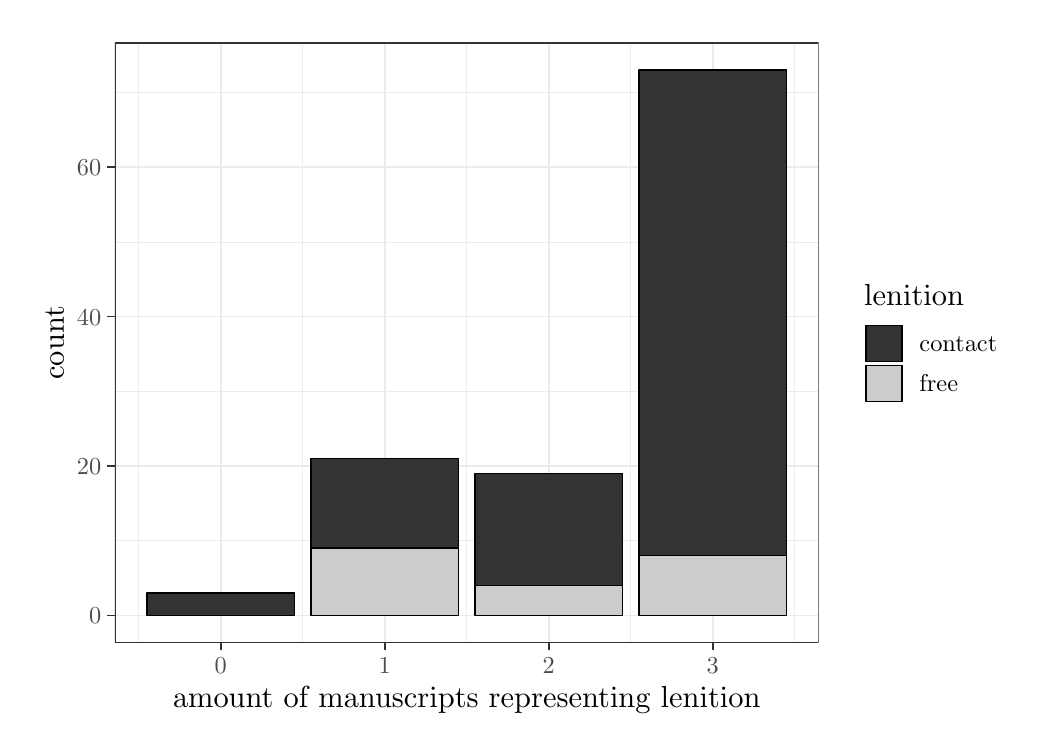
\begin{tikzpicture}[x=1pt,y=1pt]
\definecolor{fillColor}{RGB}{255,255,255}
\path[use as bounding box,fill=fillColor,fill opacity=0.00] (0,0) rectangle (361.35,252.94);
\begin{scope}
\path[clip] (  0.00,  0.00) rectangle (361.35,252.94);
\definecolor{drawColor}{RGB}{255,255,255}
\definecolor{fillColor}{RGB}{255,255,255}

\path[draw=drawColor,line width= 0.6pt,line join=round,line cap=round,fill=fillColor] (  0.00,  0.00) rectangle (361.35,252.94);
\end{scope}
\begin{scope}
\path[clip] ( 31.52, 30.72) rectangle (285.79,247.45);
\definecolor{fillColor}{RGB}{255,255,255}

\path[fill=fillColor] ( 31.52, 30.72) rectangle (285.79,247.45);
\definecolor{drawColor}{gray}{0.92}

\path[draw=drawColor,line width= 0.3pt,line join=round] ( 31.52, 67.56) --
	(285.79, 67.56);

\path[draw=drawColor,line width= 0.3pt,line join=round] ( 31.52,121.54) --
	(285.79,121.54);

\path[draw=drawColor,line width= 0.3pt,line join=round] ( 31.52,175.52) --
	(285.79,175.52);

\path[draw=drawColor,line width= 0.3pt,line join=round] ( 31.52,229.50) --
	(285.79,229.50);

\path[draw=drawColor,line width= 0.3pt,line join=round] ( 40.11, 30.72) --
	( 40.11,247.45);

\path[draw=drawColor,line width= 0.3pt,line join=round] ( 99.38, 30.72) --
	( 99.38,247.45);

\path[draw=drawColor,line width= 0.3pt,line join=round] (158.65, 30.72) --
	(158.65,247.45);

\path[draw=drawColor,line width= 0.3pt,line join=round] (217.93, 30.72) --
	(217.93,247.45);

\path[draw=drawColor,line width= 0.3pt,line join=round] (277.20, 30.72) --
	(277.20,247.45);

\path[draw=drawColor,line width= 0.6pt,line join=round] ( 31.52, 40.58) --
	(285.79, 40.58);

\path[draw=drawColor,line width= 0.6pt,line join=round] ( 31.52, 94.55) --
	(285.79, 94.55);

\path[draw=drawColor,line width= 0.6pt,line join=round] ( 31.52,148.53) --
	(285.79,148.53);

\path[draw=drawColor,line width= 0.6pt,line join=round] ( 31.52,202.51) --
	(285.79,202.51);

\path[draw=drawColor,line width= 0.6pt,line join=round] ( 69.75, 30.72) --
	( 69.75,247.45);

\path[draw=drawColor,line width= 0.6pt,line join=round] (129.02, 30.72) --
	(129.02,247.45);

\path[draw=drawColor,line width= 0.6pt,line join=round] (188.29, 30.72) --
	(188.29,247.45);

\path[draw=drawColor,line width= 0.6pt,line join=round] (247.56, 30.72) --
	(247.56,247.45);
\definecolor{drawColor}{RGB}{0,0,0}
\definecolor{fillColor}{gray}{0.20}

\path[draw=drawColor,line width= 0.6pt,line join=round,fill=fillColor] ( 43.08, 40.58) rectangle ( 96.42, 48.67);
\definecolor{fillColor}{gray}{0.80}

\path[draw=drawColor,line width= 0.6pt,line join=round,fill=fillColor] (102.35, 40.58) rectangle (155.69, 64.87);
\definecolor{fillColor}{gray}{0.20}

\path[draw=drawColor,line width= 0.6pt,line join=round,fill=fillColor] (102.35, 64.87) rectangle (155.69, 97.25);
\definecolor{fillColor}{gray}{0.80}

\path[draw=drawColor,line width= 0.6pt,line join=round,fill=fillColor] (161.62, 40.58) rectangle (214.96, 51.37);
\definecolor{fillColor}{gray}{0.20}

\path[draw=drawColor,line width= 0.6pt,line join=round,fill=fillColor] (161.62, 51.37) rectangle (214.96, 91.85);
\definecolor{fillColor}{gray}{0.80}

\path[draw=drawColor,line width= 0.6pt,line join=round,fill=fillColor] (220.89, 40.58) rectangle (274.23, 62.17);
\definecolor{fillColor}{gray}{0.20}

\path[draw=drawColor,line width= 0.6pt,line join=round,fill=fillColor] (220.89, 62.17) rectangle (274.23,237.59);
\definecolor{drawColor}{gray}{0.20}

\path[draw=drawColor,line width= 0.6pt,line join=round,line cap=round] ( 31.52, 30.72) rectangle (285.79,247.45);
\end{scope}
\begin{scope}
\path[clip] (  0.00,  0.00) rectangle (361.35,252.94);
\definecolor{drawColor}{gray}{0.30}

\node[text=drawColor,anchor=base east,inner sep=0pt, outer sep=0pt, scale=  0.88] at ( 26.57, 37.55) {0};

\node[text=drawColor,anchor=base east,inner sep=0pt, outer sep=0pt, scale=  0.88] at ( 26.57, 91.52) {20};

\node[text=drawColor,anchor=base east,inner sep=0pt, outer sep=0pt, scale=  0.88] at ( 26.57,145.50) {40};

\node[text=drawColor,anchor=base east,inner sep=0pt, outer sep=0pt, scale=  0.88] at ( 26.57,199.48) {60};
\end{scope}
\begin{scope}
\path[clip] (  0.00,  0.00) rectangle (361.35,252.94);
\definecolor{drawColor}{gray}{0.20}

\path[draw=drawColor,line width= 0.6pt,line join=round] ( 28.77, 40.58) --
	( 31.52, 40.58);

\path[draw=drawColor,line width= 0.6pt,line join=round] ( 28.77, 94.55) --
	( 31.52, 94.55);

\path[draw=drawColor,line width= 0.6pt,line join=round] ( 28.77,148.53) --
	( 31.52,148.53);

\path[draw=drawColor,line width= 0.6pt,line join=round] ( 28.77,202.51) --
	( 31.52,202.51);
\end{scope}
\begin{scope}
\path[clip] (  0.00,  0.00) rectangle (361.35,252.94);
\definecolor{drawColor}{gray}{0.20}

\path[draw=drawColor,line width= 0.6pt,line join=round] ( 69.75, 27.97) --
	( 69.75, 30.72);

\path[draw=drawColor,line width= 0.6pt,line join=round] (129.02, 27.97) --
	(129.02, 30.72);

\path[draw=drawColor,line width= 0.6pt,line join=round] (188.29, 27.97) --
	(188.29, 30.72);

\path[draw=drawColor,line width= 0.6pt,line join=round] (247.56, 27.97) --
	(247.56, 30.72);
\end{scope}
\begin{scope}
\path[clip] (  0.00,  0.00) rectangle (361.35,252.94);
\definecolor{drawColor}{gray}{0.30}

\node[text=drawColor,anchor=base,inner sep=0pt, outer sep=0pt, scale=  0.88] at ( 69.75, 19.71) {0};

\node[text=drawColor,anchor=base,inner sep=0pt, outer sep=0pt, scale=  0.88] at (129.02, 19.71) {1};

\node[text=drawColor,anchor=base,inner sep=0pt, outer sep=0pt, scale=  0.88] at (188.29, 19.71) {2};

\node[text=drawColor,anchor=base,inner sep=0pt, outer sep=0pt, scale=  0.88] at (247.56, 19.71) {3};
\end{scope}
\begin{scope}
\path[clip] (  0.00,  0.00) rectangle (361.35,252.94);
\definecolor{drawColor}{RGB}{0,0,0}

\node[text=drawColor,anchor=base,inner sep=0pt, outer sep=0pt, scale=  1.10] at (158.65,  7.44) {amount of manuscripts representing lenition};
\end{scope}
\begin{scope}
\path[clip] (  0.00,  0.00) rectangle (361.35,252.94);
\definecolor{drawColor}{RGB}{0,0,0}

\node[text=drawColor,rotate= 90.00,anchor=base,inner sep=0pt, outer sep=0pt, scale=  1.10] at ( 13.08,139.08) {count};
\end{scope}
\begin{scope}
\path[clip] (  0.00,  0.00) rectangle (361.35,252.94);
\definecolor{fillColor}{RGB}{255,255,255}

\path[fill=fillColor] (296.79,111.62) rectangle (355.85,166.55);
\end{scope}
\begin{scope}
\path[clip] (  0.00,  0.00) rectangle (361.35,252.94);
\definecolor{drawColor}{RGB}{0,0,0}

\node[text=drawColor,anchor=base west,inner sep=0pt, outer sep=0pt, scale=  1.10] at (302.29,152.50) {lenition};
\end{scope}
\begin{scope}
\path[clip] (  0.00,  0.00) rectangle (361.35,252.94);
\definecolor{fillColor}{RGB}{255,255,255}

\path[fill=fillColor] (302.29,131.57) rectangle (316.75,146.03);
\end{scope}
\begin{scope}
\path[clip] (  0.00,  0.00) rectangle (361.35,252.94);
\definecolor{drawColor}{RGB}{0,0,0}
\definecolor{fillColor}{gray}{0.20}

\path[draw=drawColor,line width= 0.6pt,line cap=round,fill=fillColor] (303.00,132.29) rectangle (316.03,145.32);
\end{scope}
\begin{scope}
\path[clip] (  0.00,  0.00) rectangle (361.35,252.94);
\definecolor{fillColor}{RGB}{255,255,255}

\path[fill=fillColor] (302.29,117.12) rectangle (316.75,131.57);
\end{scope}
\begin{scope}
\path[clip] (  0.00,  0.00) rectangle (361.35,252.94);
\definecolor{drawColor}{RGB}{0,0,0}
\definecolor{fillColor}{gray}{0.80}

\path[draw=drawColor,line width= 0.6pt,line cap=round,fill=fillColor] (303.00,117.83) rectangle (316.03,130.86);
\end{scope}
\begin{scope}
\path[clip] (  0.00,  0.00) rectangle (361.35,252.94);
\definecolor{drawColor}{RGB}{0,0,0}

\node[text=drawColor,anchor=base west,inner sep=0pt, outer sep=0pt, scale=  0.88] at (322.25,135.77) {contact};
\end{scope}
\begin{scope}
\path[clip] (  0.00,  0.00) rectangle (361.35,252.94);
\definecolor{drawColor}{RGB}{0,0,0}

\node[text=drawColor,anchor=base west,inner sep=0pt, outer sep=0pt, scale=  0.88] at (322.25,121.32) {free};
\end{scope}
\end{tikzpicture}


\end{knitrout}

\begin{knitrout}
\definecolor{shadecolor}{rgb}{0.969, 0.969, 0.969}\begin{kframe}
\begin{alltt}
\hlstd{unique.df.dewi} \hlkwb{<-} \hlstd{df.dewi} \hlopt
    \hlkwd{filter}\hlstd{(}\hlopt{!}\hlstd{((df.dewi[,}\hlnum{5}\hlstd{]} \hlopt{==} \hlstd{df.dewi[,}\hlnum{6}\hlstd{])} \hlopt{&} \hlstd{(df.dewi[,}\hlnum{6}\hlstd{]} \hlopt{==} \hlstd{df.dewi[,}\hlnum{7}\hlstd{])))}\hlopt
        \hlkwd{cbind}\hlstd{(}\hlkwd{data.frame}\hlstd{(}\hlstr{"unique"}\hlstd{=}\hlkwd{rep}\hlstd{(}\hlstr{"unique"}\hlstd{,} \hlkwd{nrow}\hlstd{(.))))}

\hlstd{notunique.df.dewi} \hlkwb{<-} \hlstd{df.dewi} \hlopt
    \hlkwd{cbind}\hlstd{(}\hlkwd{data.frame}\hlstd{(}\hlstr{"unique"}\hlstd{=}\hlkwd{rep}\hlstd{(}\hlstr{"not unique"}\hlstd{,} \hlkwd{nrow}\hlstd{(.))))}


\hlkwd{rbind}\hlstd{(unique.df.dewi, notunique.df.dewi)}\hlopt
    \hlkwd{gather}\hlstd{(}\hlkwc{key}\hlstd{=MS,}\hlkwc{value}\hlstd{=represented,}\hlnum{5}\hlopt{:}\hlnum{7}\hlstd{)} \hlopt
    \hlkwd{ggplot}\hlstd{(}\hlkwd{aes}\hlstd{(}\hlkwc{x}\hlstd{=MS,}\hlkwc{fill}\hlstd{=represented))}\hlopt{+}
    \hlkwd{xlab}\hlstd{(}\hlstr{"manuscript"}\hlstd{)}\hlopt{+}
    \hlkwd{geom_histogram}\hlstd{(}\hlkwc{stat}\hlstd{=}\hlstr{"count"}\hlstd{,}\hlkwc{binwidth}\hlstd{=}\hlnum{1}\hlstd{)}\hlopt{+}
    \hlkwd{facet_grid}\hlstd{(unique}\hlopt{~}\hlstd{lenition)}
\end{alltt}


{\ttfamily\noindent\color{warningcolor}{\#\# Warning: Ignoring unknown parameters: binwidth, bins, pad}}\end{kframe}
% Created by tikzDevice version 0.11 on 2018-12-11 10:42:22
% !TEX encoding = UTF-8 Unicode
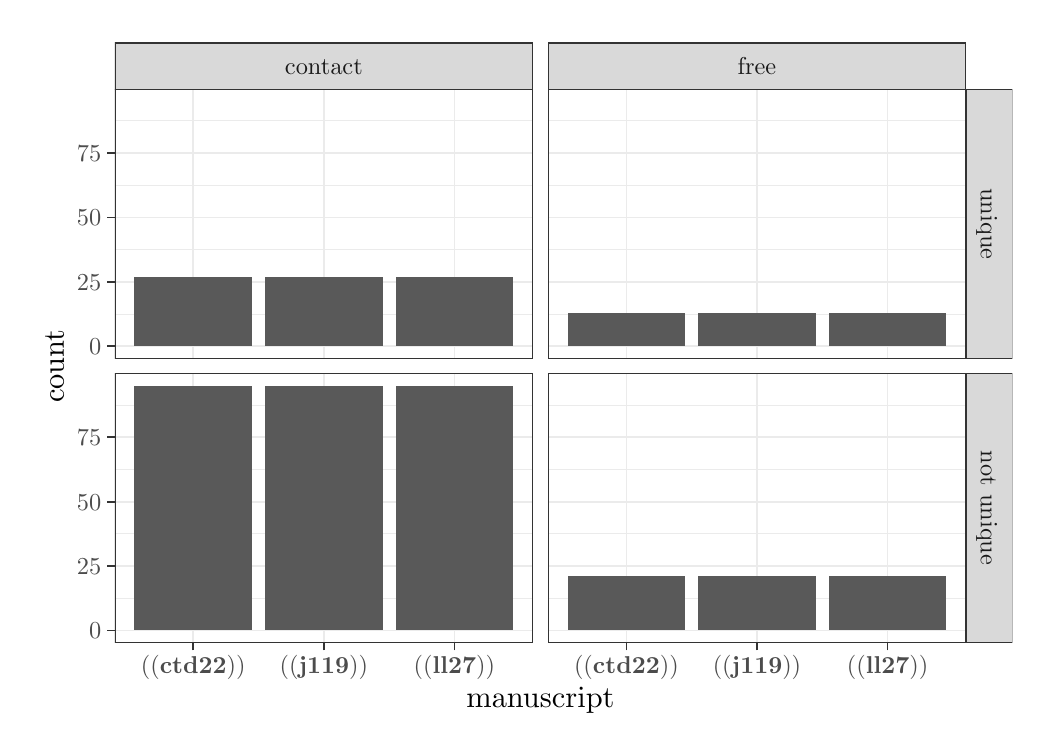
\begin{tikzpicture}[x=1pt,y=1pt]
\definecolor{fillColor}{RGB}{255,255,255}
\path[use as bounding box,fill=fillColor,fill opacity=0.00] (0,0) rectangle (361.35,252.94);
\begin{scope}
\path[clip] (  0.00,  0.00) rectangle (361.35,252.94);
\definecolor{drawColor}{RGB}{255,255,255}
\definecolor{fillColor}{RGB}{255,255,255}

\path[draw=drawColor,line width= 0.6pt,line join=round,line cap=round,fill=fillColor] (  0.00, -0.00) rectangle (361.35,252.94);
\end{scope}
\begin{scope}
\path[clip] ( 31.52,133.43) rectangle (182.53,230.64);
\definecolor{fillColor}{RGB}{255,255,255}

\path[fill=fillColor] ( 31.52,133.43) rectangle (182.53,230.64);
\definecolor{drawColor}{gray}{0.92}

\path[draw=drawColor,line width= 0.3pt,line join=round] ( 31.52,149.48) --
	(182.53,149.48);

\path[draw=drawColor,line width= 0.3pt,line join=round] ( 31.52,172.73) --
	(182.53,172.73);

\path[draw=drawColor,line width= 0.3pt,line join=round] ( 31.52,195.99) --
	(182.53,195.99);

\path[draw=drawColor,line width= 0.3pt,line join=round] ( 31.52,219.25) --
	(182.53,219.25);

\path[draw=drawColor,line width= 0.6pt,line join=round] ( 31.52,137.85) --
	(182.53,137.85);

\path[draw=drawColor,line width= 0.6pt,line join=round] ( 31.52,161.11) --
	(182.53,161.11);

\path[draw=drawColor,line width= 0.6pt,line join=round] ( 31.52,184.36) --
	(182.53,184.36);

\path[draw=drawColor,line width= 0.6pt,line join=round] ( 31.52,207.62) --
	(182.53,207.62);

\path[draw=drawColor,line width= 0.6pt,line join=round] ( 59.83,133.43) --
	( 59.83,230.64);

\path[draw=drawColor,line width= 0.6pt,line join=round] (107.02,133.43) --
	(107.02,230.64);

\path[draw=drawColor,line width= 0.6pt,line join=round] (154.22,133.43) --
	(154.22,230.64);
\definecolor{fillColor}{gray}{0.35}

\path[fill=fillColor] ( 38.60,137.85) rectangle ( 81.07,162.97);

\path[fill=fillColor] ( 85.79,137.85) rectangle (128.26,162.97);

\path[fill=fillColor] (132.98,137.85) rectangle (175.45,162.97);
\definecolor{drawColor}{gray}{0.20}

\path[draw=drawColor,line width= 0.6pt,line join=round,line cap=round] ( 31.52,133.43) rectangle (182.53,230.64);
\end{scope}
\begin{scope}
\path[clip] ( 31.52, 30.72) rectangle (182.53,127.93);
\definecolor{fillColor}{RGB}{255,255,255}

\path[fill=fillColor] ( 31.52, 30.72) rectangle (182.53,127.93);
\definecolor{drawColor}{gray}{0.92}

\path[draw=drawColor,line width= 0.3pt,line join=round] ( 31.52, 46.77) --
	(182.53, 46.77);

\path[draw=drawColor,line width= 0.3pt,line join=round] ( 31.52, 70.03) --
	(182.53, 70.03);

\path[draw=drawColor,line width= 0.3pt,line join=round] ( 31.52, 93.28) --
	(182.53, 93.28);

\path[draw=drawColor,line width= 0.3pt,line join=round] ( 31.52,116.54) --
	(182.53,116.54);

\path[draw=drawColor,line width= 0.6pt,line join=round] ( 31.52, 35.14) --
	(182.53, 35.14);

\path[draw=drawColor,line width= 0.6pt,line join=round] ( 31.52, 58.40) --
	(182.53, 58.40);

\path[draw=drawColor,line width= 0.6pt,line join=round] ( 31.52, 81.65) --
	(182.53, 81.65);

\path[draw=drawColor,line width= 0.6pt,line join=round] ( 31.52,104.91) --
	(182.53,104.91);

\path[draw=drawColor,line width= 0.6pt,line join=round] ( 59.83, 30.72) --
	( 59.83,127.93);

\path[draw=drawColor,line width= 0.6pt,line join=round] (107.02, 30.72) --
	(107.02,127.93);

\path[draw=drawColor,line width= 0.6pt,line join=round] (154.22, 30.72) --
	(154.22,127.93);
\definecolor{fillColor}{gray}{0.35}

\path[fill=fillColor] ( 38.60, 35.14) rectangle ( 81.07,123.51);

\path[fill=fillColor] ( 85.79, 35.14) rectangle (128.26,123.51);

\path[fill=fillColor] (132.98, 35.14) rectangle (175.45,123.51);
\definecolor{drawColor}{gray}{0.20}

\path[draw=drawColor,line width= 0.6pt,line join=round,line cap=round] ( 31.52, 30.72) rectangle (182.53,127.93);
\end{scope}
\begin{scope}
\path[clip] (188.03,133.43) rectangle (339.05,230.64);
\definecolor{fillColor}{RGB}{255,255,255}

\path[fill=fillColor] (188.03,133.43) rectangle (339.05,230.64);
\definecolor{drawColor}{gray}{0.92}

\path[draw=drawColor,line width= 0.3pt,line join=round] (188.03,149.48) --
	(339.05,149.48);

\path[draw=drawColor,line width= 0.3pt,line join=round] (188.03,172.73) --
	(339.05,172.73);

\path[draw=drawColor,line width= 0.3pt,line join=round] (188.03,195.99) --
	(339.05,195.99);

\path[draw=drawColor,line width= 0.3pt,line join=round] (188.03,219.25) --
	(339.05,219.25);

\path[draw=drawColor,line width= 0.6pt,line join=round] (188.03,137.85) --
	(339.05,137.85);

\path[draw=drawColor,line width= 0.6pt,line join=round] (188.03,161.11) --
	(339.05,161.11);

\path[draw=drawColor,line width= 0.6pt,line join=round] (188.03,184.36) --
	(339.05,184.36);

\path[draw=drawColor,line width= 0.6pt,line join=round] (188.03,207.62) --
	(339.05,207.62);

\path[draw=drawColor,line width= 0.6pt,line join=round] (216.35,133.43) --
	(216.35,230.64);

\path[draw=drawColor,line width= 0.6pt,line join=round] (263.54,133.43) --
	(263.54,230.64);

\path[draw=drawColor,line width= 0.6pt,line join=round] (310.73,133.43) --
	(310.73,230.64);
\definecolor{fillColor}{gray}{0.35}

\path[fill=fillColor] (195.11,137.85) rectangle (237.58,149.94);

\path[fill=fillColor] (242.30,137.85) rectangle (284.77,149.94);

\path[fill=fillColor] (289.49,137.85) rectangle (331.97,149.94);
\definecolor{drawColor}{gray}{0.20}

\path[draw=drawColor,line width= 0.6pt,line join=round,line cap=round] (188.03,133.43) rectangle (339.05,230.64);
\end{scope}
\begin{scope}
\path[clip] (188.03, 30.72) rectangle (339.05,127.93);
\definecolor{fillColor}{RGB}{255,255,255}

\path[fill=fillColor] (188.03, 30.72) rectangle (339.05,127.93);
\definecolor{drawColor}{gray}{0.92}

\path[draw=drawColor,line width= 0.3pt,line join=round] (188.03, 46.77) --
	(339.05, 46.77);

\path[draw=drawColor,line width= 0.3pt,line join=round] (188.03, 70.03) --
	(339.05, 70.03);

\path[draw=drawColor,line width= 0.3pt,line join=round] (188.03, 93.28) --
	(339.05, 93.28);

\path[draw=drawColor,line width= 0.3pt,line join=round] (188.03,116.54) --
	(339.05,116.54);

\path[draw=drawColor,line width= 0.6pt,line join=round] (188.03, 35.14) --
	(339.05, 35.14);

\path[draw=drawColor,line width= 0.6pt,line join=round] (188.03, 58.40) --
	(339.05, 58.40);

\path[draw=drawColor,line width= 0.6pt,line join=round] (188.03, 81.65) --
	(339.05, 81.65);

\path[draw=drawColor,line width= 0.6pt,line join=round] (188.03,104.91) --
	(339.05,104.91);

\path[draw=drawColor,line width= 0.6pt,line join=round] (216.35, 30.72) --
	(216.35,127.93);

\path[draw=drawColor,line width= 0.6pt,line join=round] (263.54, 30.72) --
	(263.54,127.93);

\path[draw=drawColor,line width= 0.6pt,line join=round] (310.73, 30.72) --
	(310.73,127.93);
\definecolor{fillColor}{gray}{0.35}

\path[fill=fillColor] (195.11, 35.14) rectangle (237.58, 54.68);

\path[fill=fillColor] (242.30, 35.14) rectangle (284.77, 54.68);

\path[fill=fillColor] (289.49, 35.14) rectangle (331.97, 54.68);
\definecolor{drawColor}{gray}{0.20}

\path[draw=drawColor,line width= 0.6pt,line join=round,line cap=round] (188.03, 30.72) rectangle (339.05,127.93);
\end{scope}
\begin{scope}
\path[clip] ( 31.52,230.64) rectangle (182.53,247.45);
\definecolor{drawColor}{gray}{0.20}
\definecolor{fillColor}{gray}{0.85}

\path[draw=drawColor,line width= 0.6pt,line join=round,line cap=round,fill=fillColor] ( 31.52,230.64) rectangle (182.53,247.44);
\definecolor{drawColor}{gray}{0.10}

\node[text=drawColor,anchor=base,inner sep=0pt, outer sep=0pt, scale=  0.88] at (107.02,236.01) {contact};
\end{scope}
\begin{scope}
\path[clip] (188.03,230.64) rectangle (339.05,247.45);
\definecolor{drawColor}{gray}{0.20}
\definecolor{fillColor}{gray}{0.85}

\path[draw=drawColor,line width= 0.6pt,line join=round,line cap=round,fill=fillColor] (188.03,230.64) rectangle (339.05,247.44);
\definecolor{drawColor}{gray}{0.10}

\node[text=drawColor,anchor=base,inner sep=0pt, outer sep=0pt, scale=  0.88] at (263.54,236.01) {free};
\end{scope}
\begin{scope}
\path[clip] (339.05,133.43) rectangle (355.85,230.64);
\definecolor{drawColor}{gray}{0.20}
\definecolor{fillColor}{gray}{0.85}

\path[draw=drawColor,line width= 0.6pt,line join=round,line cap=round,fill=fillColor] (339.05,133.43) rectangle (355.85,230.64);
\definecolor{drawColor}{gray}{0.10}

\node[text=drawColor,rotate=-90.00,anchor=base,inner sep=0pt, outer sep=0pt, scale=  0.88] at (344.42,182.04) {unique};
\end{scope}
\begin{scope}
\path[clip] (339.05, 30.72) rectangle (355.85,127.93);
\definecolor{drawColor}{gray}{0.20}
\definecolor{fillColor}{gray}{0.85}

\path[draw=drawColor,line width= 0.6pt,line join=round,line cap=round,fill=fillColor] (339.05, 30.72) rectangle (355.85,127.93);
\definecolor{drawColor}{gray}{0.10}

\node[text=drawColor,rotate=-90.00,anchor=base,inner sep=0pt, outer sep=0pt, scale=  0.88] at (344.42, 79.33) {not unique};
\end{scope}
\begin{scope}
\path[clip] (  0.00,  0.00) rectangle (361.35,252.94);
\definecolor{drawColor}{gray}{0.20}

\path[draw=drawColor,line width= 0.6pt,line join=round] ( 59.83, 27.97) --
	( 59.83, 30.72);

\path[draw=drawColor,line width= 0.6pt,line join=round] (107.02, 27.97) --
	(107.02, 30.72);

\path[draw=drawColor,line width= 0.6pt,line join=round] (154.22, 27.97) --
	(154.22, 30.72);
\end{scope}
\begin{scope}
\path[clip] (  0.00,  0.00) rectangle (361.35,252.94);
\definecolor{drawColor}{gray}{0.30}

\node[text=drawColor,anchor=base,inner sep=0pt, outer sep=0pt, scale=  0.88] at ( 59.83, 19.71) {\gls{ctd22}};

\node[text=drawColor,anchor=base,inner sep=0pt, outer sep=0pt, scale=  0.88] at (107.02, 19.71) {\gls{j119}};

\node[text=drawColor,anchor=base,inner sep=0pt, outer sep=0pt, scale=  0.88] at (154.22, 19.71) {\gls{ll27}};
\end{scope}
\begin{scope}
\path[clip] (  0.00,  0.00) rectangle (361.35,252.94);
\definecolor{drawColor}{gray}{0.20}

\path[draw=drawColor,line width= 0.6pt,line join=round] (216.35, 27.97) --
	(216.35, 30.72);

\path[draw=drawColor,line width= 0.6pt,line join=round] (263.54, 27.97) --
	(263.54, 30.72);

\path[draw=drawColor,line width= 0.6pt,line join=round] (310.73, 27.97) --
	(310.73, 30.72);
\end{scope}
\begin{scope}
\path[clip] (  0.00,  0.00) rectangle (361.35,252.94);
\definecolor{drawColor}{gray}{0.30}

\node[text=drawColor,anchor=base,inner sep=0pt, outer sep=0pt, scale=  0.88] at (216.35, 19.71) {\gls{ctd22}};

\node[text=drawColor,anchor=base,inner sep=0pt, outer sep=0pt, scale=  0.88] at (263.54, 19.71) {\gls{j119}};

\node[text=drawColor,anchor=base,inner sep=0pt, outer sep=0pt, scale=  0.88] at (310.73, 19.71) {\gls{ll27}};
\end{scope}
\begin{scope}
\path[clip] (  0.00,  0.00) rectangle (361.35,252.94);
\definecolor{drawColor}{gray}{0.30}

\node[text=drawColor,anchor=base east,inner sep=0pt, outer sep=0pt, scale=  0.88] at ( 26.57,134.82) {0};

\node[text=drawColor,anchor=base east,inner sep=0pt, outer sep=0pt, scale=  0.88] at ( 26.57,158.08) {25};

\node[text=drawColor,anchor=base east,inner sep=0pt, outer sep=0pt, scale=  0.88] at ( 26.57,181.33) {50};

\node[text=drawColor,anchor=base east,inner sep=0pt, outer sep=0pt, scale=  0.88] at ( 26.57,204.59) {75};
\end{scope}
\begin{scope}
\path[clip] (  0.00,  0.00) rectangle (361.35,252.94);
\definecolor{drawColor}{gray}{0.20}

\path[draw=drawColor,line width= 0.6pt,line join=round] ( 28.77,137.85) --
	( 31.52,137.85);

\path[draw=drawColor,line width= 0.6pt,line join=round] ( 28.77,161.11) --
	( 31.52,161.11);

\path[draw=drawColor,line width= 0.6pt,line join=round] ( 28.77,184.36) --
	( 31.52,184.36);

\path[draw=drawColor,line width= 0.6pt,line join=round] ( 28.77,207.62) --
	( 31.52,207.62);
\end{scope}
\begin{scope}
\path[clip] (  0.00,  0.00) rectangle (361.35,252.94);
\definecolor{drawColor}{gray}{0.30}

\node[text=drawColor,anchor=base east,inner sep=0pt, outer sep=0pt, scale=  0.88] at ( 26.57, 32.11) {0};

\node[text=drawColor,anchor=base east,inner sep=0pt, outer sep=0pt, scale=  0.88] at ( 26.57, 55.37) {25};

\node[text=drawColor,anchor=base east,inner sep=0pt, outer sep=0pt, scale=  0.88] at ( 26.57, 78.62) {50};

\node[text=drawColor,anchor=base east,inner sep=0pt, outer sep=0pt, scale=  0.88] at ( 26.57,101.88) {75};
\end{scope}
\begin{scope}
\path[clip] (  0.00,  0.00) rectangle (361.35,252.94);
\definecolor{drawColor}{gray}{0.20}

\path[draw=drawColor,line width= 0.6pt,line join=round] ( 28.77, 35.14) --
	( 31.52, 35.14);

\path[draw=drawColor,line width= 0.6pt,line join=round] ( 28.77, 58.40) --
	( 31.52, 58.40);

\path[draw=drawColor,line width= 0.6pt,line join=round] ( 28.77, 81.65) --
	( 31.52, 81.65);

\path[draw=drawColor,line width= 0.6pt,line join=round] ( 28.77,104.91) --
	( 31.52,104.91);
\end{scope}
\begin{scope}
\path[clip] (  0.00,  0.00) rectangle (361.35,252.94);
\definecolor{drawColor}{RGB}{0,0,0}

\node[text=drawColor,anchor=base,inner sep=0pt, outer sep=0pt, scale=  1.10] at (185.28,  7.44) {manuscript};
\end{scope}
\begin{scope}
\path[clip] (  0.00,  0.00) rectangle (361.35,252.94);
\definecolor{drawColor}{RGB}{0,0,0}

\node[text=drawColor,rotate= 90.00,anchor=base,inner sep=0pt, outer sep=0pt, scale=  1.10] at ( 13.08,130.68) {count};
\end{scope}
\end{tikzpicture}


\end{knitrout}

\begin{knitrout}
\definecolor{shadecolor}{rgb}{0.969, 0.969, 0.969}\begin{kframe}
\begin{alltt}
\hlstd{euler.dewi.free} \hlkwb{<-} \hlkwd{euler}\hlstd{(dewi.free[,}\hlnum{5}\hlopt{:}\hlnum{7}\hlstd{],} \hlkwc{shape}\hlstd{=}\hlstr{"ellipse"}\hlstd{)}
\hlstd{euler.dewi.free}
\end{alltt}
\begin{verbatim}
##                                      original fitted residuals regionError
## \\gls{j119}                                 2  2.001    -0.001           0
## \\gls{ll27}                                 7  7.002    -0.002           0
## \\gls{ctd22}                                0  0.000     0.000           0
## \\gls{j119}&\\gls{ll27}                     0  0.002    -0.002           0
## \\gls{j119}&\\gls{ctd22}                    0  0.001    -0.001           0
## \\gls{ll27}&\\gls{ctd22}                    4  4.001    -0.001           0
## \\gls{j119}&\\gls{ll27}&\\gls{ctd22}        8  8.003    -0.003           0
## 
## diagError: 0 
## stress:    0
\end{verbatim}
\begin{alltt}
\hlstd{euler.dewi.free} \hlopt \hlkwd{plot}\hlstd{(}\hlkwc{fill}\hlstd{=}\hlkwd{c}\hlstd{(}\hlstr{"#33EEEE"}\hlstd{,}\hlstr{"#EE33EE"}\hlstd{,} \hlstr{"#EEEE33"}\hlstd{),}
                         \hlkwc{fills}\hlstd{=}\hlnum{.25}\hlstd{,}
                         \hlkwc{cex}\hlstd{=}\hlnum{.8}\hlstd{,}
                         \hlcom{#labels="plain",}
                         \hlkwc{quantities}\hlstd{=}\hlnum{TRUE}\hlstd{,}
                         \hlcom{#legend=list(space="bottom",columns=3,alpha=1)}
                         \hlstd{)}
\end{alltt}
\end{kframe}
% Created by tikzDevice version 0.11 on 2018-12-11 10:42:24
% !TEX encoding = UTF-8 Unicode
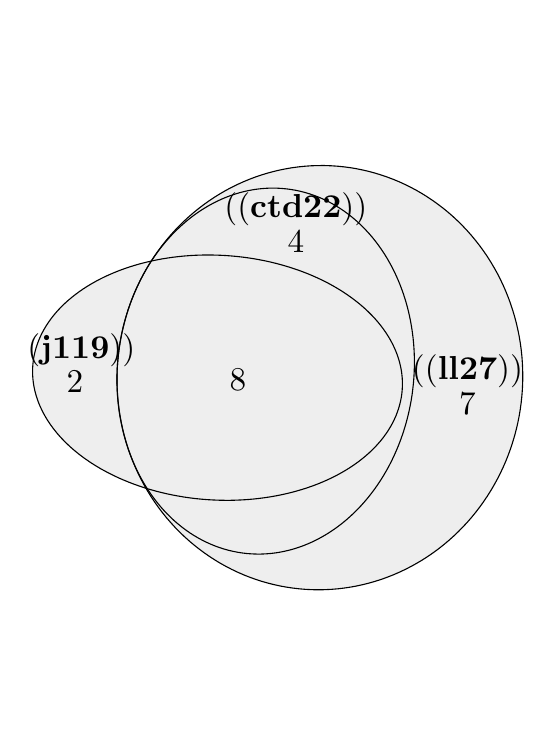
\begin{tikzpicture}[x=1pt,y=1pt]
\definecolor{fillColor}{RGB}{255,255,255}
\path[use as bounding box,fill=fillColor,fill opacity=0.00] (0,0) rectangle (180.67,252.94);
\begin{scope}
\path[clip] (  0.00,  0.00) rectangle (180.67,252.94);
\definecolor{fillColor}{RGB}{238,238,238}

\path[fill=fillColor,nonzero rule]
	( 42.04, 87.76) --
	( 40.92, 89.87) --
	( 39.86, 92.01) --
	( 38.87, 94.19) --
	( 37.94, 96.40) --
	( 37.59, 97.30) --
	( 37.29, 98.07) --
	( 36.59, 99.93) --
	( 35.95,101.82) --
	( 35.36,103.74) --
	( 34.82,105.68) --
	( 34.33,107.65) --
	( 33.89,109.64) --
	( 33.50,111.65) --
	( 33.16,113.67) --
	( 32.88,115.71) --
	( 32.65,117.76) --
	( 32.47,119.82) --
	( 32.35,121.90) --
	( 32.28,123.98) --
	( 32.26,126.06) --
	( 32.28,126.91) --
	( 32.28,127.03) --
	( 32.29,127.25) --
	( 32.30,128.15) --
	( 32.33,128.84) --
	( 32.35,129.45) --
	( 32.38,130.01) --
	( 32.39,130.23) --
	( 32.42,130.59) --
	( 32.49,131.87) --
	( 32.71,134.28) --
	( 33.00,136.68) --
	( 33.36,139.08) --
	( 33.79,141.46) --
	( 34.30,143.82) --
	( 34.88,146.17) --
	( 35.52,148.50) --
	( 35.88,149.65) --
	( 36.20,150.69) --
	( 36.22,150.74) --
	( 36.24,150.81) --
	( 36.34,151.09) --
	( 36.86,152.65) --
	( 37.01,153.06) --
	( 37.02,153.09) --
	( 37.05,153.15) --
	( 37.57,154.59) --
	( 38.33,156.50) --
	( 39.14,158.38) --
	( 40.00,160.23) --
	( 40.89,162.05) --
	( 41.84,163.84) --
	( 41.91,163.97) --
	( 41.96,164.06) --
	( 43.14,166.15) --
	( 44.38,168.20) --
	( 44.64,168.60) --
	( 44.36,168.54) --
	( 42.41,168.08) --
	( 40.48,167.58) --
	( 38.58,167.03) --
	( 36.71,166.45) --
	( 34.87,165.82) --
	( 33.07,165.16) --
	( 31.30,164.45) --
	( 29.57,163.71) --
	( 27.87,162.94) --
	( 26.22,162.12) --
	( 24.61,161.27) --
	( 23.05,160.39) --
	( 21.52,159.47) --
	( 20.05,158.52) --
	( 18.63,157.54) --
	( 17.25,156.52) --
	( 15.93,155.48) --
	( 14.65,154.41) --
	( 13.43,153.31) --
	( 12.27,152.18) --
	( 11.16,151.03) --
	( 10.11,149.85) --
	(  9.12,148.65) --
	(  8.19,147.43) --
	(  7.32,146.18) --
	(  6.51,144.92) --
	(  5.76,143.64) --
	(  5.07,142.34) --
	(  4.45,141.03) --
	(  3.89,139.70) --
	(  3.40,138.35) --
	(  2.97,137.00) --
	(  2.60,135.64) --
	(  2.30,134.26) --
	(  2.07,132.88) --
	(  1.90,131.49) --
	(  1.80,130.10) --
	(  1.77,128.70) --
	(  1.80,127.31) --
	(  1.90,125.91) --
	(  2.07,124.51) --
	(  2.30,123.11) --
	(  2.60,121.72) --
	(  2.97,120.33) --
	(  3.40,118.94) --
	(  3.89,117.57) --
	(  4.45,116.20) --
	(  5.08,114.85) --
	(  5.76,113.50) --
	(  6.51,112.17) --
	(  7.32,110.85) --
	(  8.20,109.55) --
	(  9.13,108.27) --
	( 10.12,107.00) --
	( 11.17,105.75) --
	( 12.28,104.53) --
	( 13.44,103.32) --
	( 14.66,102.14) --
	( 15.93,100.98) --
	( 17.26, 99.85) --
	( 18.64, 98.74) --
	( 20.06, 97.67) --
	( 21.54, 96.62) --
	( 23.06, 95.60) --
	( 24.62, 94.61) --
	( 26.23, 93.65) --
	( 27.89, 92.73) --
	( 29.58, 91.84) --
	( 31.31, 90.98) --
	( 33.08, 90.16) --
	( 34.88, 89.38) --
	( 36.72, 88.63) --
	( 38.59, 87.92) --
	( 40.49, 87.25) --
	( 42.42, 86.61) --
	( 42.75, 86.51) --
	cycle;

\path[fill=fillColor,nonzero rule]
	(107.40, 49.86) --
	(109.72, 49.98) --
	(112.03, 50.17) --
	(114.33, 50.44) --
	(116.62, 50.78) --
	(118.91, 51.20) --
	(121.17, 51.70) --
	(123.43, 52.26) --
	(125.66, 52.91) --
	(127.88, 53.62) --
	(130.07, 54.41) --
	(132.24, 55.27) --
	(134.39, 56.21) --
	(136.50, 57.21) --
	(138.58, 58.28) --
	(140.63, 59.42) --
	(142.65, 60.62) --
	(144.63, 61.89) --
	(146.57, 63.23) --
	(148.47, 64.63) --
	(150.32, 66.09) --
	(152.13, 67.61) --
	(153.90, 69.19) --
	(155.62, 70.83) --
	(157.28, 72.52) --
	(158.90, 74.26) --
	(160.46, 76.06) --
	(161.97, 77.91) --
	(163.42, 79.81) --
	(164.81, 81.75) --
	(166.15, 83.74) --
	(167.42, 85.77) --
	(168.63, 87.84) --
	(169.78, 89.95) --
	(170.87, 92.09) --
	(171.89, 94.27) --
	(172.85, 96.48) --
	(173.73, 98.72) --
	(174.55,100.99) --
	(175.30,103.29) --
	(175.99,105.61) --
	(176.60,107.95) --
	(177.14,110.30) --
	(177.61,112.68) --
	(178.00,115.06) --
	(178.33,117.46) --
	(178.58,119.87) --
	(178.76,122.28) --
	(178.87,124.70) --
	(178.90,127.12) --
	(178.86,129.54) --
	(178.75,131.96) --
	(178.57,134.37) --
	(178.31,136.77) --
	(177.98,139.16) --
	(177.58,141.54) --
	(177.10,143.91) --
	(176.56,146.26) --
	(175.94,148.58) --
	(175.25,150.89) --
	(174.50,153.17) --
	(173.67,155.43) --
	(172.78,157.65) --
	(171.82,159.85) --
	(170.80,162.01) --
	(169.71,164.14) --
	(168.55,166.22) --
	(167.33,168.27) --
	(166.06,170.28) --
	(164.72,172.24) --
	(163.32,174.16) --
	(161.86,176.03) --
	(160.35,177.85) --
	(158.79,179.62) --
	(157.17,181.34) --
	(155.50,183.00) --
	(153.78,184.61) --
	(152.01,186.16) --
	(150.19,187.65) --
	(148.33,189.07) --
	(146.43,190.44) --
	(144.49,191.74) --
	(142.51,192.98) --
	(140.49,194.15) --
	(138.44,195.25) --
	(136.35,196.28) --
	(134.24,197.25) --
	(132.09,198.14) --
	(129.92,198.96) --
	(127.73,199.71) --
	(125.51,200.39) --
	(123.27,201.00) --
	(121.02,201.52) --
	(118.75,201.98) --
	(116.46,202.36) --
	(114.17,202.66) --
	(111.86,202.89) --
	(109.56,203.04) --
	(107.24,203.12) --
	(104.93,203.11) --
	(102.61,203.04) --
	(100.30,202.88) --
	( 98.00,202.65) --
	( 95.70,202.35) --
	( 93.41,201.96) --
	( 91.13,201.51) --
	( 88.87,200.97) --
	( 86.63,200.37) --
	( 84.40,199.69) --
	( 82.20,198.94) --
	( 80.01,198.11) --
	( 77.86,197.21) --
	( 75.73,196.25) --
	( 73.63,195.21) --
	( 71.56,194.11) --
	( 69.53,192.93) --
	( 67.53,191.69) --
	( 65.57,190.39) --
	( 63.65,189.02) --
	( 61.78,187.59) --
	( 59.94,186.10) --
	( 58.15,184.55) --
	( 56.41,182.94) --
	( 54.72,181.28) --
	( 53.08,179.56) --
	( 51.49,177.79) --
	( 49.95,175.97) --
	( 48.48,174.09) --
	( 47.05,172.17) --
	( 45.69,170.21) --
	( 44.64,168.60) --
	( 44.69,168.61) --
	( 44.93,168.99) --
	( 46.05,170.63) --
	( 47.20,172.23) --
	( 48.39,173.78) --
	( 49.63,175.29) --
	( 50.89,176.75) --
	( 52.19,178.17) --
	( 53.53,179.53) --
	( 54.90,180.85) --
	( 56.30,182.11) --
	( 57.73,183.32) --
	( 59.18,184.48) --
	( 60.67,185.58) --
	( 62.17,186.62) --
	( 63.71,187.61) --
	( 65.26,188.53) --
	( 66.84,189.40) --
	( 68.43,190.21) --
	( 70.04,190.96) --
	( 71.67,191.64) --
	( 73.31,192.26) --
	( 74.97,192.82) --
	( 76.63,193.32) --
	( 78.31,193.75) --
	( 79.99,194.11) --
	( 81.68,194.42) --
	( 83.37,194.65) --
	( 85.07,194.82) --
	( 86.77,194.93) --
	( 88.46,194.96) --
	( 90.16,194.94) --
	( 91.84,194.84) --
	( 93.53,194.68) --
	( 95.20,194.46) --
	( 96.87,194.17) --
	( 98.53,193.81) --
	(100.17,193.39) --
	(101.80,192.91) --
	(103.41,192.36) --
	(105.01,191.75) --
	(106.59,191.07) --
	(108.14,190.34) --
	(109.68,189.54) --
	(111.19,188.68) --
	(112.68,187.76) --
	(114.14,186.79) --
	(115.57,185.75) --
	(116.97,184.66) --
	(118.34,183.52) --
	(119.68,182.31) --
	(120.98,181.06) --
	(122.25,179.75) --
	(123.49,178.40) --
	(124.69,176.99) --
	(125.84,175.54) --
	(126.96,174.03) --
	(128.04,172.49) --
	(129.08,170.90) --
	(130.07,169.27) --
	(131.02,167.59) --
	(131.92,165.88) --
	(132.78,164.14) --
	(133.59,162.35) --
	(134.36,160.54) --
	(135.07,158.69) --
	(135.74,156.81) --
	(136.36,154.91) --
	(136.93,152.98) --
	(137.44,151.02) --
	(137.91,149.04) --
	(138.32,147.04) --
	(138.68,145.03) --
	(138.99,143.00) --
	(139.25,140.95) --
	(139.45,138.89) --
	(139.60,136.83) --
	(139.70,134.75) --
	(139.74,132.67) --
	(139.73,130.58) --
	(139.67,128.49) --
	(139.55,126.41) --
	(139.38,124.32) --
	(139.15,122.24) --
	(138.88,120.17) --
	(138.55,118.10) --
	(138.16,116.05) --
	(137.73,114.01) --
	(137.24,111.98) --
	(136.71,109.97) --
	(136.12,107.98) --
	(135.48,106.01) --
	(134.79,104.06) --
	(134.06,102.14) --
	(133.27,100.24) --
	(132.44, 98.37) --
	(131.57, 96.54) --
	(130.65, 94.73) --
	(129.68, 92.96) --
	(128.67, 91.23) --
	(127.62, 89.53) --
	(126.52, 87.87) --
	(125.39, 86.25) --
	(124.21, 84.68) --
	(123.00, 83.14) --
	(121.75, 81.66) --
	(120.47, 80.22) --
	(119.15, 78.83) --
	(117.80, 77.49) --
	(116.41, 76.20) --
	(115.00, 74.96) --
	(113.56, 73.78) --
	(112.09, 72.65) --
	(110.59, 71.58) --
	(109.07, 70.56) --
	(107.53, 69.61) --
	(105.96, 68.71) --
	(104.38, 67.87) --
	(102.77, 67.09) --
	(101.15, 66.38) --
	( 99.52, 65.72) --
	( 97.87, 65.13) --
	( 96.21, 64.61) --
	( 94.54, 64.14) --
	( 92.86, 63.75) --
	( 91.17, 63.41) --
	( 89.48, 63.14) --
	( 87.79, 62.94) --
	( 86.09, 62.80) --
	( 84.39, 62.73) --
	( 82.70, 62.73) --
	( 81.01, 62.79) --
	( 79.32, 62.91) --
	( 77.64, 63.11) --
	( 75.97, 63.36) --
	( 74.31, 63.69) --
	( 72.66, 64.07) --
	( 71.02, 64.53) --
	( 69.40, 65.04) --
	( 67.79, 65.62) --
	( 66.21, 66.27) --
	( 64.64, 66.97) --
	( 63.09, 67.74) --
	( 61.57, 68.57) --
	( 60.07, 69.45) --
	( 58.60, 70.40) --
	( 57.15, 71.41) --
	( 55.74, 72.47) --
	( 54.35, 73.59) --
	( 52.99, 74.76) --
	( 51.67, 75.99) --
	( 50.38, 77.27) --
	( 49.13, 78.60) --
	( 47.91, 79.99) --
	( 46.74, 81.42) --
	( 45.60, 82.89) --
	( 44.50, 84.42) --
	( 43.44, 85.99) --
	( 43.20, 86.38) --
	( 42.75, 86.51) --
	( 43.22, 85.69) --
	( 44.47, 83.66) --
	( 45.78, 81.68) --
	( 47.15, 79.74) --
	( 48.58, 77.84) --
	( 50.06, 75.99) --
	( 51.60, 74.20) --
	( 53.19, 72.45) --
	( 54.84, 70.76) --
	( 56.53, 69.13) --
	( 58.28, 67.55) --
	( 60.07, 66.03) --
	( 61.91, 64.58) --
	( 63.79, 63.18) --
	( 65.71, 61.85) --
	( 67.67, 60.58) --
	( 69.67, 59.37) --
	( 71.71, 58.24) --
	( 73.78, 57.17) --
	( 75.88, 56.17) --
	( 78.01, 55.24) --
	( 80.17, 54.38) --
	( 82.35, 53.60) --
	( 84.56, 52.88) --
	( 86.78, 52.24) --
	( 89.03, 51.68) --
	( 91.29, 51.18) --
	( 93.57, 50.77) --
	( 95.86, 50.43) --
	( 98.16, 50.16) --
	(100.46, 49.97) --
	(102.78, 49.86) --
	(105.09, 49.82) --
	cycle;

\path[fill=fillColor,nonzero rule]
	( 42.83,165.60) --
	( 43.86,167.31) --
	( 44.69,168.61) --
	( 44.64,168.60) --
	( 44.38,168.20) --
	( 43.14,166.15) --
	( 41.96,164.06) --
	( 41.91,163.97) --
	cycle
	( 37.05,153.15) --
	( 37.02,153.09) --
	( 37.01,153.06) --
	cycle
	( 36.34,151.09) --
	( 36.24,150.81) --
	( 36.22,150.74) --
	cycle
	( 32.54,132.32) --
	( 32.74,134.40) --
	( 32.99,136.48) --
	( 33.29,138.55) --
	( 33.65,140.61) --
	( 34.05,142.66) --
	( 34.51,144.69) --
	( 35.03,146.71) --
	( 35.59,148.71) --
	( 35.88,149.65) --
	( 35.52,148.50) --
	( 34.88,146.17) --
	( 34.30,143.82) --
	( 33.79,141.46) --
	( 33.36,139.08) --
	( 33.00,136.68) --
	( 32.71,134.28) --
	( 32.49,131.87) --
	( 32.42,130.59) --
	cycle
	( 32.38,130.01) --
	( 32.35,129.45) --
	( 32.33,128.84) --
	cycle
	( 32.29,127.25) --
	( 32.28,127.03) --
	( 32.28,126.91) --
	cycle
	( 42.43, 87.60) --
	( 41.46, 89.25) --
	( 40.53, 90.94) --
	( 39.65, 92.67) --
	( 38.81, 94.44) --
	( 38.03, 96.24) --
	( 37.59, 97.30) --
	( 37.94, 96.40) --
	( 38.87, 94.19) --
	( 39.86, 92.01) --
	( 40.92, 89.87) --
	( 42.04, 87.76) --
	( 42.75, 86.51) --
	( 43.20, 86.38) --
	cycle;

\path[fill=fillColor,nonzero rule]
	( 37.88,155.35) --
	( 38.80,157.57) --
	( 39.79,159.77) --
	( 40.84,161.93) --
	( 41.91,163.97) --
	( 41.84,163.84) --
	( 40.89,162.05) --
	( 40.00,160.23) --
	( 39.14,158.38) --
	( 38.33,156.50) --
	( 37.57,154.59) --
	( 37.05,153.15) --
	cycle
	( 37.01,153.06) --
	( 36.86,152.65) --
	( 36.34,151.09) --
	cycle
	( 36.22,150.74) --
	( 36.20,150.69) --
	( 35.88,149.65) --
	cycle
	( 32.42,130.59) --
	( 32.39,130.23) --
	( 32.38,130.01) --
	cycle
	( 32.33,128.84) --
	( 32.30,128.15) --
	( 32.29,127.25) --
	cycle
	( 37.08, 98.64) --
	( 36.29,100.91) --
	( 35.57,103.20) --
	( 34.92,105.52) --
	( 34.34,107.86) --
	( 33.83,110.22) --
	( 33.39,112.59) --
	( 33.02,114.98) --
	( 32.73,117.37) --
	( 32.51,119.78) --
	( 32.36,122.20) --
	( 32.28,124.61) --
	( 32.28,126.91) --
	( 32.26,126.06) --
	( 32.28,123.98) --
	( 32.35,121.90) --
	( 32.47,119.82) --
	( 32.65,117.76) --
	( 32.88,115.71) --
	( 33.16,113.67) --
	( 33.50,111.65) --
	( 33.89,109.64) --
	( 34.33,107.65) --
	( 34.82,105.68) --
	( 35.36,103.74) --
	( 35.95,101.82) --
	( 36.59, 99.93) --
	( 37.29, 98.07) --
	( 37.59, 97.30) --
	cycle;

\path[fill=fillColor,nonzero rule]
	( 84.39, 62.73) --
	( 86.09, 62.80) --
	( 87.79, 62.94) --
	( 89.48, 63.14) --
	( 91.17, 63.41) --
	( 92.86, 63.75) --
	( 94.54, 64.14) --
	( 96.21, 64.61) --
	( 97.87, 65.13) --
	( 99.52, 65.72) --
	(101.15, 66.38) --
	(102.77, 67.09) --
	(104.38, 67.87) --
	(105.96, 68.71) --
	(107.53, 69.61) --
	(109.07, 70.56) --
	(110.59, 71.58) --
	(112.09, 72.65) --
	(113.56, 73.78) --
	(115.00, 74.96) --
	(116.41, 76.20) --
	(117.80, 77.49) --
	(119.15, 78.83) --
	(120.47, 80.22) --
	(121.75, 81.66) --
	(123.00, 83.14) --
	(124.21, 84.68) --
	(125.39, 86.25) --
	(126.52, 87.87) --
	(127.62, 89.53) --
	(128.67, 91.23) --
	(129.68, 92.96) --
	(130.65, 94.73) --
	(131.57, 96.54) --
	(132.44, 98.37) --
	(133.27,100.24) --
	(134.06,102.14) --
	(134.79,104.06) --
	(135.48,106.01) --
	(136.12,107.98) --
	(136.71,109.97) --
	(137.24,111.98) --
	(137.73,114.01) --
	(138.16,116.05) --
	(138.55,118.10) --
	(138.88,120.17) --
	(139.15,122.24) --
	(139.38,124.32) --
	(139.55,126.41) --
	(139.67,128.49) --
	(139.73,130.58) --
	(139.74,132.67) --
	(139.70,134.75) --
	(139.60,136.83) --
	(139.45,138.89) --
	(139.25,140.95) --
	(138.99,143.00) --
	(138.68,145.03) --
	(138.32,147.04) --
	(137.91,149.04) --
	(137.44,151.02) --
	(136.93,152.98) --
	(136.36,154.91) --
	(135.74,156.81) --
	(135.07,158.69) --
	(134.36,160.54) --
	(133.59,162.35) --
	(132.78,164.14) --
	(131.92,165.88) --
	(131.02,167.59) --
	(130.07,169.27) --
	(129.08,170.90) --
	(128.04,172.49) --
	(126.96,174.03) --
	(125.84,175.54) --
	(124.69,176.99) --
	(123.49,178.40) --
	(122.25,179.75) --
	(120.98,181.06) --
	(119.68,182.31) --
	(118.34,183.52) --
	(116.97,184.66) --
	(115.57,185.75) --
	(114.14,186.79) --
	(112.68,187.76) --
	(111.19,188.68) --
	(109.68,189.54) --
	(108.14,190.34) --
	(106.59,191.07) --
	(105.01,191.75) --
	(103.41,192.36) --
	(101.80,192.91) --
	(100.17,193.39) --
	( 98.53,193.81) --
	( 96.87,194.17) --
	( 95.20,194.46) --
	( 93.53,194.68) --
	( 91.84,194.84) --
	( 90.16,194.94) --
	( 88.46,194.96) --
	( 86.77,194.93) --
	( 85.07,194.82) --
	( 83.37,194.65) --
	( 81.68,194.42) --
	( 79.99,194.11) --
	( 78.31,193.75) --
	( 76.63,193.32) --
	( 74.97,192.82) --
	( 73.31,192.26) --
	( 71.67,191.64) --
	( 70.04,190.96) --
	( 68.43,190.21) --
	( 66.84,189.40) --
	( 65.26,188.53) --
	( 63.71,187.61) --
	( 62.17,186.62) --
	( 60.67,185.58) --
	( 59.18,184.48) --
	( 57.73,183.32) --
	( 56.30,182.11) --
	( 54.90,180.85) --
	( 53.53,179.53) --
	( 52.19,178.17) --
	( 50.89,176.75) --
	( 49.63,175.29) --
	( 48.39,173.78) --
	( 47.20,172.23) --
	( 46.05,170.63) --
	( 44.93,168.99) --
	( 44.69,168.61) --
	( 46.34,168.96) --
	( 48.34,169.34) --
	( 50.36,169.67) --
	( 52.40,169.97) --
	( 54.45,170.21) --
	( 56.52,170.42) --
	( 58.60,170.58) --
	( 60.69,170.70) --
	( 62.79,170.77) --
	( 64.90,170.80) --
	( 67.00,170.78) --
	( 69.11,170.72) --
	( 71.22,170.62) --
	( 73.33,170.47) --
	( 75.43,170.28) --
	( 77.53,170.05) --
	( 79.61,169.77) --
	( 81.69,169.45) --
	( 83.75,169.08) --
	( 85.80,168.68) --
	( 87.83,168.23) --
	( 89.84,167.74) --
	( 91.83,167.20) --
	( 93.79,166.63) --
	( 95.73,166.02) --
	( 97.65,165.37) --
	( 99.53,164.68) --
	(101.39,163.95) --
	(103.21,163.18) --
	(105.00,162.38) --
	(106.75,161.54) --
	(108.46,160.67) --
	(110.13,159.76) --
	(111.76,158.82) --
	(113.35,157.85) --
	(114.90,156.84) --
	(116.39,155.81) --
	(117.84,154.74) --
	(119.25,153.65) --
	(120.60,152.53) --
	(121.90,151.39) --
	(123.14,150.22) --
	(124.33,149.02) --
	(125.47,147.81) --
	(126.55,146.57) --
	(127.57,145.31) --
	(128.53,144.04) --
	(129.43,142.74) --
	(130.28,141.44) --
	(131.06,140.11) --
	(131.77,138.77) --
	(132.43,137.42) --
	(133.02,136.06) --
	(133.55,134.69) --
	(134.01,133.31) --
	(134.41,131.92) --
	(134.74,130.53) --
	(135.01,129.14) --
	(135.21,127.74) --
	(135.34,126.34) --
	(135.41,124.94) --
	(135.41,123.54) --
	(135.34,122.15) --
	(135.21,120.76) --
	(135.01,119.37) --
	(134.74,117.99) --
	(134.41,116.63) --
	(134.01,115.27) --
	(133.55,113.92) --
	(133.03,112.58) --
	(132.43,111.26) --
	(131.78,109.95) --
	(131.06,108.66) --
	(130.28,107.39) --
	(129.44,106.14) --
	(128.54,104.90) --
	(127.58,103.69) --
	(126.55,102.50) --
	(125.48,101.34) --
	(124.34,100.20) --
	(123.15, 99.08) --
	(121.90, 98.00) --
	(120.61, 96.94) --
	(119.26, 95.91) --
	(117.85, 94.91) --
	(116.40, 93.94) --
	(114.91, 93.01) --
	(113.36, 92.11) --
	(111.78, 91.24) --
	(110.14, 90.41) --
	(108.47, 89.61) --
	(106.76, 88.86) --
	(105.01, 88.13) --
	(103.22, 87.45) --
	(101.40, 86.81) --
	( 99.55, 86.20) --
	( 97.66, 85.64) --
	( 95.75, 85.11) --
	( 93.81, 84.63) --
	( 91.84, 84.19) --
	( 89.85, 83.79) --
	( 87.84, 83.43) --
	( 85.81, 83.12) --
	( 83.76, 82.85) --
	( 81.70, 82.62) --
	( 79.63, 82.44) --
	( 77.54, 82.30) --
	( 75.45, 82.21) --
	( 73.34, 82.15) --
	( 71.24, 82.15) --
	( 69.13, 82.19) --
	( 67.02, 82.27) --
	( 64.91, 82.39) --
	( 62.81, 82.56) --
	( 60.71, 82.77) --
	( 58.62, 83.03) --
	( 56.54, 83.33) --
	( 54.47, 83.68) --
	( 52.41, 84.06) --
	( 50.37, 84.49) --
	( 48.35, 84.96) --
	( 46.35, 85.47) --
	( 44.37, 86.02) --
	( 43.20, 86.38) --
	( 43.44, 85.99) --
	( 44.50, 84.42) --
	( 45.60, 82.89) --
	( 46.74, 81.42) --
	( 47.91, 79.99) --
	( 49.13, 78.60) --
	( 50.38, 77.27) --
	( 51.67, 75.99) --
	( 52.99, 74.76) --
	( 54.35, 73.59) --
	( 55.74, 72.47) --
	( 57.15, 71.41) --
	( 58.60, 70.40) --
	( 60.07, 69.45) --
	( 61.57, 68.57) --
	( 63.09, 67.74) --
	( 64.64, 66.97) --
	( 66.21, 66.27) --
	( 67.79, 65.62) --
	( 69.40, 65.04) --
	( 71.02, 64.53) --
	( 72.66, 64.07) --
	( 74.31, 63.69) --
	( 75.97, 63.36) --
	( 77.64, 63.11) --
	( 79.32, 62.91) --
	( 81.01, 62.79) --
	( 82.70, 62.73) --
	cycle;

\path[fill=fillColor,nonzero rule]
	( 73.34, 82.15) --
	( 75.45, 82.21) --
	( 77.54, 82.30) --
	( 79.63, 82.44) --
	( 81.70, 82.62) --
	( 83.76, 82.85) --
	( 85.81, 83.12) --
	( 87.84, 83.43) --
	( 89.85, 83.79) --
	( 91.84, 84.19) --
	( 93.81, 84.63) --
	( 95.75, 85.11) --
	( 97.66, 85.64) --
	( 99.55, 86.20) --
	(101.40, 86.81) --
	(103.22, 87.45) --
	(105.01, 88.13) --
	(106.76, 88.86) --
	(108.47, 89.61) --
	(110.14, 90.41) --
	(111.78, 91.24) --
	(113.36, 92.11) --
	(114.91, 93.01) --
	(116.40, 93.94) --
	(117.85, 94.91) --
	(119.26, 95.91) --
	(120.61, 96.94) --
	(121.90, 98.00) --
	(123.15, 99.08) --
	(124.34,100.20) --
	(125.48,101.34) --
	(126.55,102.50) --
	(127.58,103.69) --
	(128.54,104.90) --
	(129.44,106.14) --
	(130.28,107.39) --
	(131.06,108.66) --
	(131.78,109.95) --
	(132.43,111.26) --
	(133.03,112.58) --
	(133.55,113.92) --
	(134.01,115.27) --
	(134.41,116.63) --
	(134.74,117.99) --
	(135.01,119.37) --
	(135.21,120.76) --
	(135.34,122.15) --
	(135.41,123.54) --
	(135.41,124.94) --
	(135.34,126.34) --
	(135.21,127.74) --
	(135.01,129.14) --
	(134.74,130.53) --
	(134.41,131.92) --
	(134.01,133.31) --
	(133.55,134.69) --
	(133.02,136.06) --
	(132.43,137.42) --
	(131.77,138.77) --
	(131.06,140.11) --
	(130.28,141.44) --
	(129.43,142.74) --
	(128.53,144.04) --
	(127.57,145.31) --
	(126.55,146.57) --
	(125.47,147.81) --
	(124.33,149.02) --
	(123.14,150.22) --
	(121.90,151.39) --
	(120.60,152.53) --
	(119.25,153.65) --
	(117.84,154.74) --
	(116.39,155.81) --
	(114.90,156.84) --
	(113.35,157.85) --
	(111.76,158.82) --
	(110.13,159.76) --
	(108.46,160.67) --
	(106.75,161.54) --
	(105.00,162.38) --
	(103.21,163.18) --
	(101.39,163.95) --
	( 99.53,164.68) --
	( 97.65,165.37) --
	( 95.73,166.02) --
	( 93.79,166.63) --
	( 91.83,167.20) --
	( 89.84,167.74) --
	( 87.83,168.23) --
	( 85.80,168.68) --
	( 83.75,169.08) --
	( 81.69,169.45) --
	( 79.61,169.77) --
	( 77.53,170.05) --
	( 75.43,170.28) --
	( 73.33,170.47) --
	( 71.22,170.62) --
	( 69.11,170.72) --
	( 67.00,170.78) --
	( 64.90,170.80) --
	( 62.79,170.77) --
	( 60.69,170.70) --
	( 58.60,170.58) --
	( 56.52,170.42) --
	( 54.45,170.21) --
	( 52.40,169.97) --
	( 50.36,169.67) --
	( 48.34,169.34) --
	( 46.34,168.96) --
	( 44.69,168.61) --
	( 43.86,167.31) --
	( 42.83,165.60) --
	( 41.91,163.97) --
	( 40.84,161.93) --
	( 39.79,159.77) --
	( 38.80,157.57) --
	( 37.88,155.35) --
	( 37.05,153.15) --
	( 37.01,153.06) --
	( 36.34,151.09) --
	( 36.22,150.74) --
	( 35.88,149.65) --
	( 35.59,148.71) --
	( 35.03,146.71) --
	( 34.51,144.69) --
	( 34.05,142.66) --
	( 33.65,140.61) --
	( 33.29,138.55) --
	( 32.99,136.48) --
	( 32.74,134.40) --
	( 32.54,132.32) --
	( 32.42,130.59) --
	( 32.38,130.01) --
	( 32.33,128.84) --
	( 32.29,127.25) --
	( 32.28,126.91) --
	( 32.28,124.61) --
	( 32.36,122.20) --
	( 32.51,119.78) --
	( 32.73,117.37) --
	( 33.02,114.98) --
	( 33.39,112.59) --
	( 33.83,110.22) --
	( 34.34,107.86) --
	( 34.92,105.52) --
	( 35.57,103.20) --
	( 36.29,100.91) --
	( 37.08, 98.64) --
	( 37.59, 97.30) --
	( 38.03, 96.24) --
	( 38.81, 94.44) --
	( 39.65, 92.67) --
	( 40.53, 90.94) --
	( 41.46, 89.25) --
	( 42.43, 87.60) --
	( 43.20, 86.38) --
	( 44.37, 86.02) --
	( 46.35, 85.47) --
	( 48.35, 84.96) --
	( 50.37, 84.49) --
	( 52.41, 84.06) --
	( 54.47, 83.68) --
	( 56.54, 83.33) --
	( 58.62, 83.03) --
	( 60.71, 82.77) --
	( 62.81, 82.56) --
	( 64.91, 82.39) --
	( 67.02, 82.27) --
	( 69.13, 82.19) --
	( 71.24, 82.15) --
	cycle;
\definecolor{drawColor}{RGB}{0,0,0}

\path[draw=drawColor,line width= 0.4pt,line join=round,line cap=round] ( 71.22,170.62) --
	( 69.11,170.72) --
	( 67.00,170.78) --
	( 64.90,170.80) --
	( 62.79,170.77) --
	( 60.69,170.70) --
	( 58.60,170.58) --
	( 56.52,170.42) --
	( 54.45,170.21) --
	( 52.40,169.97) --
	( 50.36,169.67) --
	( 48.34,169.34) --
	( 46.34,168.96) --
	( 44.36,168.54) --
	( 42.41,168.08) --
	( 40.48,167.58) --
	( 38.58,167.03) --
	( 36.71,166.45) --
	( 34.87,165.82) --
	( 33.07,165.16) --
	( 31.30,164.45) --
	( 29.57,163.71) --
	( 27.87,162.94) --
	( 26.22,162.12) --
	( 24.61,161.27) --
	( 23.05,160.39) --
	( 21.52,159.47) --
	( 20.05,158.52) --
	( 18.63,157.54) --
	( 17.25,156.52) --
	( 15.93,155.48) --
	( 14.65,154.41) --
	( 13.43,153.31) --
	( 12.27,152.18) --
	( 11.16,151.03) --
	( 10.11,149.85) --
	(  9.12,148.65) --
	(  8.19,147.43) --
	(  7.32,146.18) --
	(  6.51,144.92) --
	(  5.76,143.64) --
	(  5.07,142.34) --
	(  4.45,141.03) --
	(  3.89,139.70) --
	(  3.40,138.35) --
	(  2.97,137.00) --
	(  2.60,135.64) --
	(  2.30,134.26) --
	(  2.07,132.88) --
	(  1.90,131.49) --
	(  1.80,130.10) --
	(  1.77,128.70) --
	(  1.80,127.31) --
	(  1.90,125.91) --
	(  2.07,124.51) --
	(  2.30,123.11) --
	(  2.60,121.72) --
	(  2.97,120.33) --
	(  3.40,118.94) --
	(  3.89,117.57) --
	(  4.45,116.20) --
	(  5.08,114.85) --
	(  5.76,113.50) --
	(  6.51,112.17) --
	(  7.32,110.85) --
	(  8.20,109.55) --
	(  9.13,108.27) --
	( 10.12,107.00) --
	( 11.17,105.75) --
	( 12.28,104.53) --
	( 13.44,103.32) --
	( 14.66,102.14) --
	( 15.93,100.98) --
	( 17.26, 99.85) --
	( 18.64, 98.74) --
	( 20.06, 97.67) --
	( 21.54, 96.62) --
	( 23.06, 95.60) --
	( 24.62, 94.61) --
	( 26.23, 93.65) --
	( 27.89, 92.73) --
	( 29.58, 91.84) --
	( 31.31, 90.98) --
	( 33.08, 90.16) --
	( 34.88, 89.38) --
	( 36.72, 88.63) --
	( 38.59, 87.92) --
	( 40.49, 87.25) --
	( 42.42, 86.61) --
	( 44.37, 86.02) --
	( 46.35, 85.47) --
	( 48.35, 84.96) --
	( 50.37, 84.49) --
	( 52.41, 84.06) --
	( 54.47, 83.68) --
	( 56.54, 83.33) --
	( 58.62, 83.03) --
	( 60.71, 82.77) --
	( 62.81, 82.56) --
	( 64.91, 82.39) --
	( 67.02, 82.27) --
	( 69.13, 82.19) --
	( 71.24, 82.15) --
	( 73.34, 82.15) --
	( 75.45, 82.21) --
	( 77.54, 82.30) --
	( 79.63, 82.44) --
	( 81.70, 82.62) --
	( 83.76, 82.85) --
	( 85.81, 83.12) --
	( 87.84, 83.43) --
	( 89.85, 83.79) --
	( 91.84, 84.19) --
	( 93.81, 84.63) --
	( 95.75, 85.11) --
	( 97.66, 85.64) --
	( 99.55, 86.20) --
	(101.40, 86.81) --
	(103.22, 87.45) --
	(105.01, 88.13) --
	(106.76, 88.86) --
	(108.47, 89.61) --
	(110.14, 90.41) --
	(111.78, 91.24) --
	(113.36, 92.11) --
	(114.91, 93.01) --
	(116.40, 93.94) --
	(117.85, 94.91) --
	(119.26, 95.91) --
	(120.61, 96.94) --
	(121.90, 98.00) --
	(123.15, 99.08) --
	(124.34,100.20) --
	(125.48,101.34) --
	(126.55,102.50) --
	(127.58,103.69) --
	(128.54,104.90) --
	(129.44,106.14) --
	(130.28,107.39) --
	(131.06,108.66) --
	(131.78,109.95) --
	(132.43,111.26) --
	(133.03,112.58) --
	(133.55,113.92) --
	(134.01,115.27) --
	(134.41,116.63) --
	(134.74,117.99) --
	(135.01,119.37) --
	(135.21,120.76) --
	(135.34,122.15) --
	(135.41,123.54) --
	(135.41,124.94) --
	(135.34,126.34) --
	(135.21,127.74) --
	(135.01,129.14) --
	(134.74,130.53) --
	(134.41,131.92) --
	(134.01,133.31) --
	(133.55,134.69) --
	(133.02,136.06) --
	(132.43,137.42) --
	(131.77,138.77) --
	(131.06,140.11) --
	(130.28,141.44) --
	(129.43,142.74) --
	(128.53,144.04) --
	(127.57,145.31) --
	(126.55,146.57) --
	(125.47,147.81) --
	(124.33,149.02) --
	(123.14,150.22) --
	(121.90,151.39) --
	(120.60,152.53) --
	(119.25,153.65) --
	(117.84,154.74) --
	(116.39,155.81) --
	(114.90,156.84) --
	(113.35,157.85) --
	(111.76,158.82) --
	(110.13,159.76) --
	(108.46,160.67) --
	(106.75,161.54) --
	(105.00,162.38) --
	(103.21,163.18) --
	(101.39,163.95) --
	( 99.53,164.68) --
	( 97.65,165.37) --
	( 95.73,166.02) --
	( 93.79,166.63) --
	( 91.83,167.20) --
	( 89.84,167.74) --
	( 87.83,168.23) --
	( 85.80,168.68) --
	( 83.75,169.08) --
	( 81.69,169.45) --
	( 79.61,169.77) --
	( 77.53,170.05) --
	( 75.43,170.28) --
	( 73.33,170.47) --
	( 71.22,170.62);

\path[draw=drawColor,line width= 0.4pt,line join=round,line cap=round] (111.86,202.89) --
	(109.56,203.04) --
	(107.24,203.12) --
	(104.93,203.11) --
	(102.61,203.04) --
	(100.30,202.88) --
	( 98.00,202.65) --
	( 95.70,202.35) --
	( 93.41,201.96) --
	( 91.13,201.51) --
	( 88.87,200.97) --
	( 86.63,200.37) --
	( 84.40,199.69) --
	( 82.20,198.94) --
	( 80.01,198.11) --
	( 77.86,197.21) --
	( 75.73,196.25) --
	( 73.63,195.21) --
	( 71.56,194.11) --
	( 69.53,192.93) --
	( 67.53,191.69) --
	( 65.57,190.39) --
	( 63.65,189.02) --
	( 61.78,187.59) --
	( 59.94,186.10) --
	( 58.15,184.55) --
	( 56.41,182.94) --
	( 54.72,181.28) --
	( 53.08,179.56) --
	( 51.49,177.79) --
	( 49.95,175.97) --
	( 48.48,174.09) --
	( 47.05,172.17) --
	( 45.69,170.21) --
	( 44.38,168.20) --
	( 43.14,166.15) --
	( 41.96,164.06) --
	( 40.84,161.93) --
	( 39.79,159.77) --
	( 38.80,157.57) --
	( 37.88,155.35) --
	( 37.02,153.09) --
	( 36.24,150.81) --
	( 35.52,148.50) --
	( 34.88,146.17) --
	( 34.30,143.82) --
	( 33.79,141.46) --
	( 33.36,139.08) --
	( 33.00,136.68) --
	( 32.71,134.28) --
	( 32.49,131.87) --
	( 32.35,129.45) --
	( 32.28,127.03) --
	( 32.28,124.61) --
	( 32.36,122.20) --
	( 32.51,119.78) --
	( 32.73,117.37) --
	( 33.02,114.98) --
	( 33.39,112.59) --
	( 33.83,110.22) --
	( 34.34,107.86) --
	( 34.92,105.52) --
	( 35.57,103.20) --
	( 36.29,100.91) --
	( 37.08, 98.64) --
	( 37.94, 96.40) --
	( 38.87, 94.19) --
	( 39.86, 92.01) --
	( 40.92, 89.87) --
	( 42.04, 87.76) --
	( 43.22, 85.69) --
	( 44.47, 83.66) --
	( 45.78, 81.68) --
	( 47.15, 79.74) --
	( 48.58, 77.84) --
	( 50.06, 75.99) --
	( 51.60, 74.20) --
	( 53.19, 72.45) --
	( 54.84, 70.76) --
	( 56.53, 69.13) --
	( 58.28, 67.55) --
	( 60.07, 66.03) --
	( 61.91, 64.58) --
	( 63.79, 63.18) --
	( 65.71, 61.85) --
	( 67.67, 60.58) --
	( 69.67, 59.37) --
	( 71.71, 58.24) --
	( 73.78, 57.17) --
	( 75.88, 56.17) --
	( 78.01, 55.24) --
	( 80.17, 54.38) --
	( 82.35, 53.60) --
	( 84.56, 52.88) --
	( 86.78, 52.24) --
	( 89.03, 51.68) --
	( 91.29, 51.18) --
	( 93.57, 50.77) --
	( 95.86, 50.43) --
	( 98.16, 50.16) --
	(100.46, 49.97) --
	(102.78, 49.86) --
	(105.09, 49.82) --
	(107.40, 49.86) --
	(109.72, 49.98) --
	(112.03, 50.17) --
	(114.33, 50.44) --
	(116.62, 50.78) --
	(118.91, 51.20) --
	(121.17, 51.70) --
	(123.43, 52.26) --
	(125.66, 52.91) --
	(127.88, 53.62) --
	(130.07, 54.41) --
	(132.24, 55.27) --
	(134.39, 56.21) --
	(136.50, 57.21) --
	(138.58, 58.28) --
	(140.63, 59.42) --
	(142.65, 60.62) --
	(144.63, 61.89) --
	(146.57, 63.23) --
	(148.47, 64.63) --
	(150.32, 66.09) --
	(152.13, 67.61) --
	(153.90, 69.19) --
	(155.62, 70.83) --
	(157.28, 72.52) --
	(158.90, 74.26) --
	(160.46, 76.06) --
	(161.97, 77.91) --
	(163.42, 79.81) --
	(164.81, 81.75) --
	(166.15, 83.74) --
	(167.42, 85.77) --
	(168.63, 87.84) --
	(169.78, 89.95) --
	(170.87, 92.09) --
	(171.89, 94.27) --
	(172.85, 96.48) --
	(173.73, 98.72) --
	(174.55,100.99) --
	(175.30,103.29) --
	(175.99,105.61) --
	(176.60,107.95) --
	(177.14,110.30) --
	(177.61,112.68) --
	(178.00,115.06) --
	(178.33,117.46) --
	(178.58,119.87) --
	(178.76,122.28) --
	(178.87,124.70) --
	(178.90,127.12) --
	(178.86,129.54) --
	(178.75,131.96) --
	(178.57,134.37) --
	(178.31,136.77) --
	(177.98,139.16) --
	(177.58,141.54) --
	(177.10,143.91) --
	(176.56,146.26) --
	(175.94,148.58) --
	(175.25,150.89) --
	(174.50,153.17) --
	(173.67,155.43) --
	(172.78,157.65) --
	(171.82,159.85) --
	(170.80,162.01) --
	(169.71,164.14) --
	(168.55,166.22) --
	(167.33,168.27) --
	(166.06,170.28) --
	(164.72,172.24) --
	(163.32,174.16) --
	(161.86,176.03) --
	(160.35,177.85) --
	(158.79,179.62) --
	(157.17,181.34) --
	(155.50,183.00) --
	(153.78,184.61) --
	(152.01,186.16) --
	(150.19,187.65) --
	(148.33,189.07) --
	(146.43,190.44) --
	(144.49,191.74) --
	(142.51,192.98) --
	(140.49,194.15) --
	(138.44,195.25) --
	(136.35,196.28) --
	(134.24,197.25) --
	(132.09,198.14) --
	(129.92,198.96) --
	(127.73,199.71) --
	(125.51,200.39) --
	(123.27,201.00) --
	(121.02,201.52) --
	(118.75,201.98) --
	(116.46,202.36) --
	(114.17,202.66) --
	(111.86,202.89);

\path[draw=drawColor,line width= 0.4pt,line join=round,line cap=round] ( 93.53,194.68) --
	( 91.84,194.84) --
	( 90.16,194.94) --
	( 88.46,194.96) --
	( 86.77,194.93) --
	( 85.07,194.82) --
	( 83.37,194.65) --
	( 81.68,194.42) --
	( 79.99,194.11) --
	( 78.31,193.75) --
	( 76.63,193.32) --
	( 74.97,192.82) --
	( 73.31,192.26) --
	( 71.67,191.64) --
	( 70.04,190.96) --
	( 68.43,190.21) --
	( 66.84,189.40) --
	( 65.26,188.53) --
	( 63.71,187.61) --
	( 62.17,186.62) --
	( 60.67,185.58) --
	( 59.18,184.48) --
	( 57.73,183.32) --
	( 56.30,182.11) --
	( 54.90,180.85) --
	( 53.53,179.53) --
	( 52.19,178.17) --
	( 50.89,176.75) --
	( 49.63,175.29) --
	( 48.39,173.78) --
	( 47.20,172.23) --
	( 46.05,170.63) --
	( 44.93,168.99) --
	( 43.86,167.31) --
	( 42.83,165.60) --
	( 41.84,163.84) --
	( 40.89,162.05) --
	( 40.00,160.23) --
	( 39.14,158.38) --
	( 38.33,156.50) --
	( 37.57,154.59) --
	( 36.86,152.65) --
	( 36.20,150.69) --
	( 35.59,148.71) --
	( 35.03,146.71) --
	( 34.51,144.69) --
	( 34.05,142.66) --
	( 33.65,140.61) --
	( 33.29,138.55) --
	( 32.99,136.48) --
	( 32.74,134.40) --
	( 32.54,132.32) --
	( 32.39,130.23) --
	( 32.30,128.15) --
	( 32.26,126.06) --
	( 32.28,123.98) --
	( 32.35,121.90) --
	( 32.47,119.82) --
	( 32.65,117.76) --
	( 32.88,115.71) --
	( 33.16,113.67) --
	( 33.50,111.65) --
	( 33.89,109.64) --
	( 34.33,107.65) --
	( 34.82,105.68) --
	( 35.36,103.74) --
	( 35.95,101.82) --
	( 36.59, 99.93) --
	( 37.29, 98.07) --
	( 38.03, 96.24) --
	( 38.81, 94.44) --
	( 39.65, 92.67) --
	( 40.53, 90.94) --
	( 41.46, 89.25) --
	( 42.43, 87.60) --
	( 43.44, 85.99) --
	( 44.50, 84.42) --
	( 45.60, 82.89) --
	( 46.74, 81.42) --
	( 47.91, 79.99) --
	( 49.13, 78.60) --
	( 50.38, 77.27) --
	( 51.67, 75.99) --
	( 52.99, 74.76) --
	( 54.35, 73.59) --
	( 55.74, 72.47) --
	( 57.15, 71.41) --
	( 58.60, 70.40) --
	( 60.07, 69.45) --
	( 61.57, 68.57) --
	( 63.09, 67.74) --
	( 64.64, 66.97) --
	( 66.21, 66.27) --
	( 67.79, 65.62) --
	( 69.40, 65.04) --
	( 71.02, 64.53) --
	( 72.66, 64.07) --
	( 74.31, 63.69) --
	( 75.97, 63.36) --
	( 77.64, 63.11) --
	( 79.32, 62.91) --
	( 81.01, 62.79) --
	( 82.70, 62.73) --
	( 84.39, 62.73) --
	( 86.09, 62.80) --
	( 87.79, 62.94) --
	( 89.48, 63.14) --
	( 91.17, 63.41) --
	( 92.86, 63.75) --
	( 94.54, 64.14) --
	( 96.21, 64.61) --
	( 97.87, 65.13) --
	( 99.52, 65.72) --
	(101.15, 66.38) --
	(102.77, 67.09) --
	(104.38, 67.87) --
	(105.96, 68.71) --
	(107.53, 69.61) --
	(109.07, 70.56) --
	(110.59, 71.58) --
	(112.09, 72.65) --
	(113.56, 73.78) --
	(115.00, 74.96) --
	(116.41, 76.20) --
	(117.80, 77.49) --
	(119.15, 78.83) --
	(120.47, 80.22) --
	(121.75, 81.66) --
	(123.00, 83.14) --
	(124.21, 84.68) --
	(125.39, 86.25) --
	(126.52, 87.87) --
	(127.62, 89.53) --
	(128.67, 91.23) --
	(129.68, 92.96) --
	(130.65, 94.73) --
	(131.57, 96.54) --
	(132.44, 98.37) --
	(133.27,100.24) --
	(134.06,102.14) --
	(134.79,104.06) --
	(135.48,106.01) --
	(136.12,107.98) --
	(136.71,109.97) --
	(137.24,111.98) --
	(137.73,114.01) --
	(138.16,116.05) --
	(138.55,118.10) --
	(138.88,120.17) --
	(139.15,122.24) --
	(139.38,124.32) --
	(139.55,126.41) --
	(139.67,128.49) --
	(139.73,130.58) --
	(139.74,132.67) --
	(139.70,134.75) --
	(139.60,136.83) --
	(139.45,138.89) --
	(139.25,140.95) --
	(138.99,143.00) --
	(138.68,145.03) --
	(138.32,147.04) --
	(137.91,149.04) --
	(137.44,151.02) --
	(136.93,152.98) --
	(136.36,154.91) --
	(135.74,156.81) --
	(135.07,158.69) --
	(134.36,160.54) --
	(133.59,162.35) --
	(132.78,164.14) --
	(131.92,165.88) --
	(131.02,167.59) --
	(130.07,169.27) --
	(129.08,170.90) --
	(128.04,172.49) --
	(126.96,174.03) --
	(125.84,175.54) --
	(124.69,176.99) --
	(123.49,178.40) --
	(122.25,179.75) --
	(120.98,181.06) --
	(119.68,182.31) --
	(118.34,183.52) --
	(116.97,184.66) --
	(115.57,185.75) --
	(114.14,186.79) --
	(112.68,187.76) --
	(111.19,188.68) --
	(109.68,189.54) --
	(108.14,190.34) --
	(106.59,191.07) --
	(105.01,191.75) --
	(103.41,192.36) --
	(101.80,192.91) --
	(100.17,193.39) --
	( 98.53,193.81) --
	( 96.87,194.17) --
	( 95.20,194.46) --
	( 93.53,194.68);

\node[text=drawColor,anchor=base,inner sep=0pt, outer sep=0pt, scale=  1.20] at ( 17.06,133.37) {\gls{j119}};

\node[text=drawColor,anchor=base,inner sep=0pt, outer sep=0pt, scale=  1.20] at (158.93,125.71) {\gls{ll27}};

\node[text=drawColor,anchor=base,inner sep=0pt, outer sep=0pt, scale=  1.20] at ( 96.89,184.18) {\gls{ctd22}};

\node[text=drawColor,anchor=base,inner sep=0pt, outer sep=0pt, scale=  1.20] at ( 76.01,121.90) {8};

\node[text=drawColor,anchor=base,inner sep=0pt, outer sep=0pt, scale=  1.20] at ( 17.06,120.96) {2};

\node[text=drawColor,anchor=base,inner sep=0pt, outer sep=0pt, scale=  1.20] at (158.93,113.30) {7};

\node[text=drawColor,anchor=base,inner sep=0pt, outer sep=0pt, scale=  1.20] at ( 96.89,171.78) {4};
\end{scope}
\end{tikzpicture}


\end{knitrout}

\begin{knitrout}
\definecolor{shadecolor}{rgb}{0.969, 0.969, 0.969}\begin{kframe}
\begin{alltt}
\hlkwd{colnames}\hlstd{(dewi.cont)[}\hlnum{5}\hlopt{:}\hlnum{7}\hlstd{]} \hlkwb{<-} \hlstd{glsnames}
\hlstd{euler.dewi.cont} \hlkwb{<-} \hlkwd{euler}\hlstd{(dewi.cont[,}\hlnum{5}\hlopt{:}\hlnum{7}\hlstd{],} \hlkwc{shape}\hlstd{=}\hlstr{"ellipse"}\hlstd{)}
\hlstd{euler.dewi.cont}
\end{alltt}
\begin{verbatim}
##                                      original fitted residuals regionError
## \\gls{j119}                                 1  0.998     0.002           0
## \\gls{ll27}                                 3  2.995     0.005           0
## \\gls{ctd22}                                8  7.987     0.013           0
## \\gls{j119}&\\gls{ll27}                     2  1.997     0.003           0
## \\gls{j119}&\\gls{ctd22}                    0  0.000     0.000           0
## \\gls{ll27}&\\gls{ctd22}                   13 12.979     0.021           0
## \\gls{j119}&\\gls{ll27}&\\gls{ctd22}       65 64.896     0.104           0
## 
## diagError: 0 
## stress:    0
\end{verbatim}
\begin{alltt}
\hlstd{euler.dewi.cont} \hlopt \hlkwd{plot}\hlstd{(}\hlkwc{fill}\hlstd{=}\hlkwd{c}\hlstd{(}\hlstr{"#33EEEE"}\hlstd{,}\hlstr{"#EE33EE"}\hlstd{,} \hlstr{"#EEEE33"}\hlstd{),}
                         \hlkwc{fills}\hlstd{=}\hlnum{.25}\hlstd{,}
                         \hlkwc{cex}\hlstd{=}\hlnum{.8}\hlstd{,}
                         \hlkwc{labels}\hlstd{=}\hlnum{FALSE}\hlstd{,}\hlcom{#"plain",}
                         \hlkwc{quantities}\hlstd{=}\hlnum{TRUE}\hlstd{,}
                         \hlcom{#auto.key=FALSE,}
                         \hlcom{#auto.key=list(space="bottom")}
                         \hlstd{)}
\end{alltt}
\end{kframe}
% Created by tikzDevice version 0.11 on 2018-12-11 10:42:24
% !TEX encoding = UTF-8 Unicode
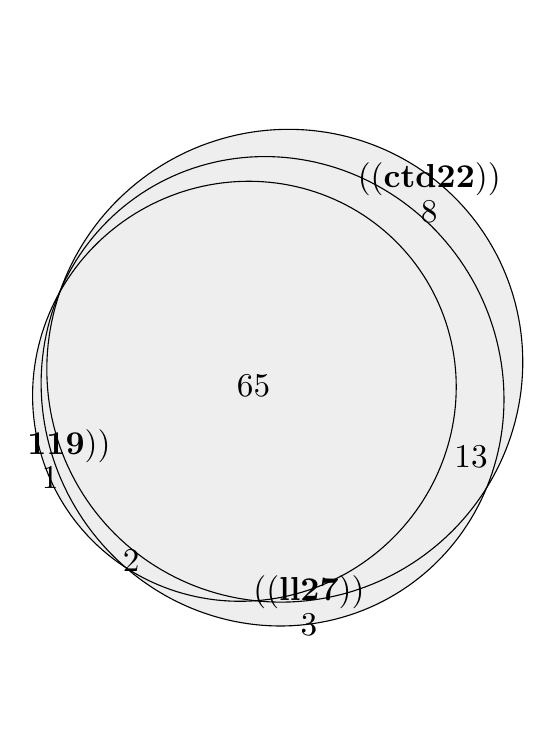
\begin{tikzpicture}[x=1pt,y=1pt]
\definecolor{fillColor}{RGB}{255,255,255}
\path[use as bounding box,fill=fillColor,fill opacity=0.00] (0,0) rectangle (180.67,252.94);
\begin{scope}
\path[clip] (  0.00,  0.00) rectangle (180.67,252.94);
\definecolor{fillColor}{RGB}{238,238,238}

\path[fill=fillColor,nonzero rule]
	( 34.24, 58.89) --
	( 32.25, 60.72) --
	( 30.33, 62.62) --
	( 28.46, 64.58) --
	( 26.65, 66.59) --
	( 24.91, 68.65) --
	( 23.22, 70.77) --
	( 21.60, 72.94) --
	( 20.05, 75.16) --
	( 18.57, 77.43) --
	( 17.16, 79.73) --
	( 15.81, 82.08) --
	( 14.54, 84.47) --
	( 13.35, 86.90) --
	( 12.22, 89.36) --
	( 11.18, 91.85) --
	( 10.21, 94.38) --
	(  9.32, 96.93) --
	(  8.51, 99.50) --
	(  7.78,102.10) --
	(  7.13,104.71) --
	(  6.56,107.35) --
	(  6.07,109.99) --
	(  5.66,112.65) --
	(  5.34,115.32) --
	(  5.10,117.99) --
	(  4.94,120.67) --
	(  4.86,123.35) --
	(  4.87,126.02) --
	(  4.96,128.69) --
	(  5.14,131.36) --
	(  5.40,134.01) --
	(  5.74,136.66) --
	(  6.16,139.28) --
	(  6.67,141.89) --
	(  7.26,144.48) --
	(  7.93,147.05) --
	(  8.67,149.59) --
	(  9.50,152.10) --
	( 10.41,154.58) --
	( 11.36,156.95) --
	( 10.81,155.96) --
	(  9.71,153.81) --
	(  8.67,151.62) --
	(  7.70,149.41) --
	(  6.80,147.16) --
	(  5.98,144.90) --
	(  5.22,142.61) --
	(  4.54,140.29) --
	(  3.94,137.96) --
	(  3.40,135.61) --
	(  2.94,133.25) --
	(  2.56,130.88) --
	(  2.25,128.50) --
	(  2.02,126.11) --
	(  1.86,123.72) --
	(  1.78,121.32) --
	(  1.78,118.92) --
	(  1.85,116.53) --
	(  2.00,114.14) --
	(  2.23,111.76) --
	(  2.53,109.39) --
	(  2.90,107.03) --
	(  3.35,104.69) --
	(  3.88,102.36) --
	(  4.48,100.05) --
	(  5.15, 97.77) --
	(  5.90, 95.50) --
	(  6.72, 93.27) --
	(  7.61, 91.06) --
	(  8.57, 88.88) --
	(  9.60, 86.73) --
	( 10.70, 84.62) --
	( 11.87, 82.55) --
	( 13.10, 80.51) --
	( 14.40, 78.52) --
	( 15.76, 76.56) --
	( 17.18, 74.66) --
	( 18.67, 72.80) --
	( 20.21, 70.99) --
	( 21.81, 69.22) --
	( 23.47, 67.52) --
	( 25.19, 65.86) --
	( 26.95, 64.26) --
	( 28.77, 62.72) --
	( 30.64, 61.23) --
	( 32.55, 59.81) --
	( 34.51, 58.45) --
	( 35.43, 57.85) --
	cycle;

\path[fill=fillColor,nonzero rule]
	( 11.67,157.51) --
	( 11.98,158.36) --
	( 11.39,157.03) --
	( 11.36,156.95) --
	cycle
	( 92.83, 36.75) --
	( 95.46, 36.84) --
	( 98.09, 37.02) --
	(100.71, 37.28) --
	(103.31, 37.62) --
	(105.90, 38.05) --
	(108.48, 38.56) --
	(111.03, 39.15) --
	(113.56, 39.83) --
	(116.07, 40.59) --
	(118.55, 41.42) --
	(120.99, 42.34) --
	(123.41, 43.34) --
	(125.79, 44.41) --
	(128.14, 45.56) --
	(130.44, 46.79) --
	(132.70, 48.09) --
	(134.92, 49.47) --
	(137.10, 50.91) --
	(139.22, 52.43) --
	(141.29, 54.02) --
	(143.31, 55.67) --
	(145.28, 57.39) --
	(147.19, 59.17) --
	(149.04, 61.02) --
	(150.83, 62.92) --
	(152.56, 64.89) --
	(154.22, 66.91) --
	(155.82, 68.98) --
	(157.36, 71.11) --
	(158.82, 73.29) --
	(160.21, 75.51) --
	(161.53, 77.79) --
	(162.78, 80.10) --
	(163.96, 82.46) --
	(165.06, 84.85) --
	(165.80, 86.62) --
	(165.48, 86.09) --
	(163.98, 83.81) --
	(162.42, 81.58) --
	(160.79, 79.40) --
	(159.09, 77.28) --
	(157.32, 75.20) --
	(155.49, 73.18) --
	(153.60, 71.22) --
	(151.64, 69.31) --
	(149.63, 67.47) --
	(147.56, 65.69) --
	(145.44, 63.98) --
	(143.26, 62.33) --
	(141.04, 60.75) --
	(138.76, 59.24) --
	(136.44, 57.80) --
	(134.08, 56.44) --
	(131.68, 55.15) --
	(129.23, 53.93) --
	(126.76, 52.79) --
	(124.24, 51.73) --
	(121.70, 50.75) --
	(119.13, 49.85) --
	(116.53, 49.02) --
	(113.91, 48.28) --
	(111.26, 47.63) --
	(108.60, 47.05) --
	(105.92, 46.56) --
	(103.23, 46.15) --
	(100.53, 45.83) --
	( 97.83, 45.59) --
	( 95.11, 45.43) --
	( 92.40, 45.36) --
	( 89.68, 45.38) --
	( 86.97, 45.48) --
	( 84.27, 45.67) --
	( 82.32, 45.86) --
	( 80.01, 45.73) --
	( 77.60, 45.66) --
	( 75.18, 45.68) --
	( 72.77, 45.76) --
	( 70.36, 45.93) --
	( 67.96, 46.16) --
	( 65.57, 46.48) --
	( 63.20, 46.87) --
	( 60.83, 47.33) --
	( 58.49, 47.87) --
	( 56.17, 48.48) --
	( 53.86, 49.16) --
	( 51.59, 49.91) --
	( 49.34, 50.74) --
	( 47.11, 51.64) --
	( 44.92, 52.60) --
	( 42.76, 53.64) --
	( 40.64, 54.74) --
	( 38.56, 55.91) --
	( 36.51, 57.15) --
	( 35.43, 57.85) --
	( 36.27, 57.12) --
	( 38.36, 55.41) --
	( 40.50, 53.76) --
	( 42.69, 52.19) --
	( 44.92, 50.68) --
	( 47.19, 49.25) --
	( 49.51, 47.88) --
	( 51.86, 46.59) --
	( 54.26, 45.38) --
	( 56.68, 44.24) --
	( 59.14, 43.18) --
	( 61.63, 42.19) --
	( 64.14, 41.29) --
	( 66.68, 40.46) --
	( 69.24, 39.72) --
	( 71.82, 39.05) --
	( 74.41, 38.47) --
	( 77.02, 37.98) --
	( 79.64, 37.56) --
	( 82.27, 37.23) --
	( 84.91, 36.98) --
	( 87.55, 36.82) --
	( 90.19, 36.74) --
	cycle;

\path[fill=fillColor,nonzero rule]
	(166.90, 88.41) --
	(168.24, 90.77) --
	(169.51, 93.17) --
	(170.71, 95.61) --
	(171.83, 98.09) --
	(172.87,100.60) --
	(173.83,103.14) --
	(174.70,105.70) --
	(175.50,108.29) --
	(176.22,110.90) --
	(176.85,113.54) --
	(177.40,116.19) --
	(177.86,118.85) --
	(178.24,121.53) --
	(178.53,124.21) --
	(178.74,126.90) --
	(178.87,129.60) --
	(178.90,132.30) --
	(178.86,134.99) --
	(178.72,137.68) --
	(178.50,140.37) --
	(178.20,143.04) --
	(177.81,145.71) --
	(177.33,148.35) --
	(176.77,150.98) --
	(176.13,153.60) --
	(175.41,156.18) --
	(174.60,158.74) --
	(173.71,161.28) --
	(172.74,163.78) --
	(171.69,166.25) --
	(170.57,168.69) --
	(169.36,171.09) --
	(168.08,173.44) --
	(166.72,175.76) --
	(165.29,178.03) --
	(163.79,180.25) --
	(162.22,182.43) --
	(160.58,184.55) --
	(158.87,186.62) --
	(157.10,188.63) --
	(155.26,190.59) --
	(153.36,192.48) --
	(151.40,194.32) --
	(149.38,196.09) --
	(147.30,197.79) --
	(145.17,199.43) --
	(142.99,201.00) --
	(140.76,202.51) --
	(138.48,203.93) --
	(136.15,205.29) --
	(133.78,206.57) --
	(131.38,207.78) --
	(128.93,208.91) --
	(126.45,209.96) --
	(123.93,210.93) --
	(121.38,211.83) --
	(118.81,212.64) --
	(116.20,213.37) --
	(113.58,214.02) --
	(110.93,214.58) --
	(108.27,215.07) --
	(105.59,215.46) --
	(102.90,215.78) --
	(100.20,216.01) --
	( 97.49,216.15) --
	( 94.78,216.21) --
	( 92.06,216.18) --
	( 89.35,216.07) --
	( 86.64,215.87) --
	( 83.93,215.59) --
	( 81.24,215.23) --
	( 78.55,214.78) --
	( 75.88,214.24) --
	( 73.23,213.62) --
	( 70.60,212.92) --
	( 67.99,212.14) --
	( 65.40,211.28) --
	( 62.84,210.34) --
	( 60.32,209.32) --
	( 57.82,208.22) --
	( 55.36,207.04) --
	( 52.94,205.78) --
	( 50.55,204.46) --
	( 48.21,203.05) --
	( 45.91,201.58) --
	( 43.66,200.04) --
	( 41.46,198.42) --
	( 39.31,196.74) --
	( 37.22,194.99) --
	( 35.18,193.18) --
	( 33.19,191.31) --
	( 31.27,189.38) --
	( 29.41,187.39) --
	( 27.61,185.34) --
	( 25.87,183.24) --
	( 24.21,181.08) --
	( 22.61,178.88) --
	( 21.08,176.62) --
	( 19.62,174.32) --
	( 18.24,171.98) --
	( 16.93,169.60) --
	( 15.70,167.18) --
	( 14.54,164.72) --
	( 13.46,162.23) --
	( 12.46,159.71) --
	( 11.98,158.36) --
	( 12.46,159.45) --
	( 13.59,161.82) --
	( 14.81,164.16) --
	( 16.09,166.45) --
	( 17.45,168.70) --
	( 18.88,170.90) --
	( 20.38,173.06) --
	( 21.94,175.16) --
	( 23.57,177.21) --
	( 25.27,179.20) --
	( 27.03,181.13) --
	( 28.85,183.01) --
	( 30.73,184.82) --
	( 32.67,186.58) --
	( 34.66,188.26) --
	( 36.71,189.88) --
	( 38.81,191.43) --
	( 40.96,192.92) --
	( 43.16,194.33) --
	( 45.40,195.67) --
	( 47.68,196.93) --
	( 50.01,198.12) --
	( 52.37,199.23) --
	( 54.77,200.27) --
	( 57.20,201.23) --
	( 59.66,202.10) --
	( 62.16,202.90) --
	( 64.68,203.62) --
	( 67.22,204.25) --
	( 69.78,204.81) --
	( 72.36,205.27) --
	( 74.96,205.66) --
	( 77.58,205.96) --
	( 80.20,206.18) --
	( 82.83,206.31) --
	( 85.47,206.36) --
	( 88.11,206.33) --
	( 90.75,206.21) --
	( 93.38,206.00) --
	( 96.02,205.71) --
	( 98.64,205.34) --
	(101.26,204.88) --
	(103.86,204.35) --
	(106.45,203.72) --
	(109.02,203.02) --
	(111.57,202.24) --
	(114.09,201.37) --
	(116.59,200.43) --
	(119.07,199.40) --
	(121.51,198.30) --
	(123.92,197.12) --
	(126.29,195.87) --
	(128.63,194.54) --
	(130.92,193.14) --
	(133.18,191.67) --
	(135.39,190.13) --
	(137.55,188.52) --
	(139.66,186.85) --
	(141.73,185.10) --
	(143.73,183.30) --
	(145.69,181.43) --
	(147.59,179.51) --
	(149.43,177.52) --
	(151.20,175.48) --
	(152.92,173.39) --
	(154.57,171.25) --
	(156.15,169.05) --
	(157.67,166.81) --
	(159.12,164.52) --
	(160.50,162.19) --
	(161.81,159.82) --
	(163.04,157.42) --
	(164.20,154.97) --
	(165.28,152.49) --
	(166.29,149.99) --
	(167.22,147.45) --
	(168.07,144.89) --
	(168.84,142.30) --
	(169.53,139.69) --
	(170.14,137.07) --
	(170.67,134.43) --
	(171.12,131.78) --
	(171.49,129.11) --
	(171.77,126.44) --
	(171.97,123.77) --
	(172.08,121.09) --
	(172.12,118.41) --
	(172.07,115.74) --
	(171.93,113.07) --
	(171.72,110.41) --
	(171.42,107.76) --
	(171.03,105.13) --
	(170.57,102.51) --
	(170.02, 99.91) --
	(169.39, 97.33) --
	(168.68, 94.78) --
	(167.90, 92.25) --
	(167.03, 89.75) --
	(166.08, 87.29) --
	(165.80, 86.62) --
	cycle;

\path[fill=fillColor,nonzero rule]
	( 80.01, 45.73) --
	( 82.32, 45.86) --
	( 81.57, 45.94) --
	( 78.89, 46.29) --
	( 76.22, 46.73) --
	( 73.56, 47.26) --
	( 70.92, 47.86) --
	( 68.31, 48.55) --
	( 65.72, 49.33) --
	( 63.16, 50.18) --
	( 60.63, 51.11) --
	( 58.13, 52.12) --
	( 55.66, 53.21) --
	( 53.23, 54.38) --
	( 50.85, 55.63) --
	( 48.50, 56.95) --
	( 46.20, 58.34) --
	( 43.94, 59.80) --
	( 41.73, 61.34) --
	( 39.58, 62.95) --
	( 37.47, 64.62) --
	( 35.43, 66.36) --
	( 33.44, 68.16) --
	( 31.50, 70.03) --
	( 29.63, 71.95) --
	( 27.83, 73.94) --
	( 26.09, 75.98) --
	( 24.41, 78.07) --
	( 22.80, 80.22) --
	( 21.27, 82.42) --
	( 19.80, 84.67) --
	( 18.41, 86.96) --
	( 17.09, 89.30) --
	( 15.85, 91.68) --
	( 14.68, 94.09) --
	( 13.59, 96.55) --
	( 12.58, 99.03) --
	( 11.65,101.55) --
	( 10.81,104.10) --
	( 10.04,106.68) --
	(  9.36,109.28) --
	(  8.75,111.90) --
	(  8.24,114.54) --
	(  7.81,117.19) --
	(  7.46,119.86) --
	(  7.20,122.54) --
	(  7.02,125.23) --
	(  6.93,127.92) --
	(  6.92,130.62) --
	(  7.00,133.32) --
	(  7.17,136.01) --
	(  7.42,138.70) --
	(  7.76,141.38) --
	(  8.18,144.05) --
	(  8.69,146.71) --
	(  9.28,149.35) --
	(  9.95,151.97) --
	( 10.71,154.58) --
	( 11.54,157.15) --
	( 11.67,157.51) --
	( 11.36,156.95) --
	( 10.41,154.58) --
	(  9.50,152.10) --
	(  8.67,149.59) --
	(  7.93,147.05) --
	(  7.26,144.48) --
	(  6.67,141.89) --
	(  6.16,139.28) --
	(  5.74,136.66) --
	(  5.40,134.01) --
	(  5.14,131.36) --
	(  4.96,128.69) --
	(  4.87,126.02) --
	(  4.86,123.35) --
	(  4.94,120.67) --
	(  5.10,117.99) --
	(  5.34,115.32) --
	(  5.66,112.65) --
	(  6.07,109.99) --
	(  6.56,107.35) --
	(  7.13,104.71) --
	(  7.78,102.10) --
	(  8.51, 99.50) --
	(  9.32, 96.93) --
	( 10.21, 94.38) --
	( 11.18, 91.85) --
	( 12.22, 89.36) --
	( 13.35, 86.90) --
	( 14.54, 84.47) --
	( 15.81, 82.08) --
	( 17.16, 79.73) --
	( 18.57, 77.43) --
	( 20.05, 75.16) --
	( 21.60, 72.94) --
	( 23.22, 70.77) --
	( 24.91, 68.65) --
	( 26.65, 66.59) --
	( 28.46, 64.58) --
	( 30.33, 62.62) --
	( 32.25, 60.72) --
	( 34.24, 58.89) --
	( 35.43, 57.85) --
	( 36.51, 57.15) --
	( 38.56, 55.91) --
	( 40.64, 54.74) --
	( 42.76, 53.64) --
	( 44.92, 52.60) --
	( 47.11, 51.64) --
	( 49.34, 50.74) --
	( 51.59, 49.91) --
	( 53.86, 49.16) --
	( 56.17, 48.48) --
	( 58.49, 47.87) --
	( 60.83, 47.33) --
	( 63.20, 46.87) --
	( 65.57, 46.48) --
	( 67.96, 46.16) --
	( 70.36, 45.93) --
	( 72.77, 45.76) --
	( 75.18, 45.68) --
	( 77.60, 45.66) --
	cycle;

\path[fill=fillColor,nonzero rule]
	( 95.11, 45.43) --
	( 97.83, 45.59) --
	(100.53, 45.83) --
	(103.23, 46.15) --
	(105.92, 46.56) --
	(108.60, 47.05) --
	(111.26, 47.63) --
	(113.91, 48.28) --
	(116.53, 49.02) --
	(119.13, 49.85) --
	(121.70, 50.75) --
	(124.24, 51.73) --
	(126.76, 52.79) --
	(129.23, 53.93) --
	(131.68, 55.15) --
	(134.08, 56.44) --
	(136.44, 57.80) --
	(138.76, 59.24) --
	(141.04, 60.75) --
	(143.26, 62.33) --
	(145.44, 63.98) --
	(147.56, 65.69) --
	(149.63, 67.47) --
	(151.64, 69.31) --
	(153.60, 71.22) --
	(155.49, 73.18) --
	(157.32, 75.20) --
	(159.09, 77.28) --
	(160.79, 79.40) --
	(162.42, 81.58) --
	(163.98, 83.81) --
	(165.48, 86.09) --
	(165.80, 86.62) --
	(166.08, 87.29) --
	(167.03, 89.75) --
	(167.90, 92.25) --
	(168.68, 94.78) --
	(169.39, 97.33) --
	(170.02, 99.91) --
	(170.57,102.51) --
	(171.03,105.13) --
	(171.42,107.76) --
	(171.72,110.41) --
	(171.93,113.07) --
	(172.07,115.74) --
	(172.12,118.41) --
	(172.08,121.09) --
	(171.97,123.77) --
	(171.77,126.44) --
	(171.49,129.11) --
	(171.12,131.78) --
	(170.67,134.43) --
	(170.14,137.07) --
	(169.53,139.69) --
	(168.84,142.30) --
	(168.07,144.89) --
	(167.22,147.45) --
	(166.29,149.99) --
	(165.28,152.49) --
	(164.20,154.97) --
	(163.04,157.42) --
	(161.81,159.82) --
	(160.50,162.19) --
	(159.12,164.52) --
	(157.67,166.81) --
	(156.15,169.05) --
	(154.57,171.25) --
	(152.92,173.39) --
	(151.20,175.48) --
	(149.43,177.52) --
	(147.59,179.51) --
	(145.69,181.43) --
	(143.73,183.30) --
	(141.73,185.10) --
	(139.66,186.85) --
	(137.55,188.52) --
	(135.39,190.13) --
	(133.18,191.67) --
	(130.92,193.14) --
	(128.63,194.54) --
	(126.29,195.87) --
	(123.92,197.12) --
	(121.51,198.30) --
	(119.07,199.40) --
	(116.59,200.43) --
	(114.09,201.37) --
	(111.57,202.24) --
	(109.02,203.02) --
	(106.45,203.72) --
	(103.86,204.35) --
	(101.26,204.88) --
	( 98.64,205.34) --
	( 96.02,205.71) --
	( 93.38,206.00) --
	( 90.75,206.21) --
	( 88.11,206.33) --
	( 85.47,206.36) --
	( 82.83,206.31) --
	( 80.20,206.18) --
	( 77.58,205.96) --
	( 74.96,205.66) --
	( 72.36,205.27) --
	( 69.78,204.81) --
	( 67.22,204.25) --
	( 64.68,203.62) --
	( 62.16,202.90) --
	( 59.66,202.10) --
	( 57.20,201.23) --
	( 54.77,200.27) --
	( 52.37,199.23) --
	( 50.01,198.12) --
	( 47.68,196.93) --
	( 45.40,195.67) --
	( 43.16,194.33) --
	( 40.96,192.92) --
	( 38.81,191.43) --
	( 36.71,189.88) --
	( 34.66,188.26) --
	( 32.67,186.58) --
	( 30.73,184.82) --
	( 28.85,183.01) --
	( 27.03,181.13) --
	( 25.27,179.20) --
	( 23.57,177.21) --
	( 21.94,175.16) --
	( 20.38,173.06) --
	( 18.88,170.90) --
	( 17.45,168.70) --
	( 16.09,166.45) --
	( 14.81,164.16) --
	( 13.59,161.82) --
	( 12.46,159.45) --
	( 11.98,158.36) --
	( 11.67,157.51) --
	( 11.98,158.08) --
	( 13.22,160.16) --
	( 14.53,162.20) --
	( 15.89,164.20) --
	( 17.32,166.16) --
	( 18.81,168.08) --
	( 20.36,169.95) --
	( 21.97,171.77) --
	( 23.64,173.54) --
	( 25.35,175.26) --
	( 27.13,176.93) --
	( 28.95,178.54) --
	( 30.82,180.09) --
	( 32.74,181.59) --
	( 34.70,183.02) --
	( 36.71,184.40) --
	( 38.76,185.71) --
	( 40.85,186.95) --
	( 42.97,188.14) --
	( 45.13,189.25) --
	( 47.33,190.30) --
	( 49.55,191.28) --
	( 51.81,192.19) --
	( 54.09,193.03) --
	( 56.39,193.80) --
	( 58.72,194.50) --
	( 61.06,195.12) --
	( 63.42,195.67) --
	( 65.80,196.15) --
	( 68.19,196.55) --
	( 70.59,196.88) --
	( 73.00,197.13) --
	( 75.41,197.31) --
	( 77.83,197.41) --
	( 80.25,197.44) --
	( 82.66,197.39) --
	( 85.07,197.26) --
	( 87.48,197.06) --
	( 89.87,196.79) --
	( 92.25,196.44) --
	( 94.62,196.01) --
	( 96.98,195.51) --
	( 99.31,194.94) --
	(101.62,194.29) --
	(103.91,193.57) --
	(106.18,192.78) --
	(108.41,191.92) --
	(110.62,190.99) --
	(112.80,189.98) --
	(114.94,188.92) --
	(117.04,187.78) --
	(119.11,186.58) --
	(121.13,185.31) --
	(123.11,183.98) --
	(125.05,182.58) --
	(126.94,181.13) --
	(128.78,179.62) --
	(130.57,178.05) --
	(132.31,176.42) --
	(134.00,174.73) --
	(135.63,173.00) --
	(137.20,171.21) --
	(138.72,169.38) --
	(140.17,167.49) --
	(141.56,165.56) --
	(142.89,163.59) --
	(144.16,161.57) --
	(145.36,159.52) --
	(146.49,157.43) --
	(147.56,155.30) --
	(148.55,153.13) --
	(149.48,150.94) --
	(150.33,148.72) --
	(151.12,146.47) --
	(151.83,144.19) --
	(152.46,141.89) --
	(153.03,139.57) --
	(153.52,137.24) --
	(153.93,134.89) --
	(154.27,132.52) --
	(154.53,130.15) --
	(154.72,127.76) --
	(154.83,125.37) --
	(154.86,122.98) --
	(154.82,120.58) --
	(154.70,118.18) --
	(154.51,115.79) --
	(154.24,113.41) --
	(153.89,111.03) --
	(153.47,108.66) --
	(152.98,106.31) --
	(152.41,103.97) --
	(151.76,101.65) --
	(151.04, 99.34) --
	(150.25, 97.06) --
	(149.39, 94.81) --
	(148.46, 92.58) --
	(147.46, 90.38) --
	(146.38, 88.21) --
	(145.25, 86.08) --
	(144.04, 83.98) --
	(142.77, 81.91) --
	(141.43, 79.89) --
	(140.03, 77.91) --
	(138.57, 75.97) --
	(137.05, 74.08) --
	(135.47, 72.23) --
	(133.84, 70.44) --
	(132.15, 68.69) --
	(130.40, 67.00) --
	(128.60, 65.36) --
	(126.76, 63.78) --
	(124.86, 62.25) --
	(122.92, 60.79) --
	(120.94, 59.38) --
	(118.91, 58.04) --
	(116.84, 56.76) --
	(114.73, 55.54) --
	(112.59, 54.40) --
	(110.41, 53.31) --
	(108.20, 52.30) --
	(105.96, 51.35) --
	(103.69, 50.48) --
	(101.40, 49.67) --
	( 99.08, 48.94) --
	( 96.75, 48.28) --
	( 94.39, 47.69) --
	( 92.02, 47.18) --
	( 89.64, 46.74) --
	( 87.24, 46.37) --
	( 84.84, 46.08) --
	( 82.43, 45.87) --
	( 82.32, 45.86) --
	( 84.27, 45.67) --
	( 86.97, 45.48) --
	( 89.68, 45.38) --
	( 92.40, 45.36) --
	cycle;

\path[fill=fillColor,nonzero rule]
	( 82.43, 45.87) --
	( 84.84, 46.08) --
	( 87.24, 46.37) --
	( 89.64, 46.74) --
	( 92.02, 47.18) --
	( 94.39, 47.69) --
	( 96.75, 48.28) --
	( 99.08, 48.94) --
	(101.40, 49.67) --
	(103.69, 50.48) --
	(105.96, 51.35) --
	(108.20, 52.30) --
	(110.41, 53.31) --
	(112.59, 54.40) --
	(114.73, 55.54) --
	(116.84, 56.76) --
	(118.91, 58.04) --
	(120.94, 59.38) --
	(122.92, 60.79) --
	(124.86, 62.25) --
	(126.76, 63.78) --
	(128.60, 65.36) --
	(130.40, 67.00) --
	(132.15, 68.69) --
	(133.84, 70.44) --
	(135.47, 72.23) --
	(137.05, 74.08) --
	(138.57, 75.97) --
	(140.03, 77.91) --
	(141.43, 79.89) --
	(142.77, 81.91) --
	(144.04, 83.98) --
	(145.25, 86.08) --
	(146.38, 88.21) --
	(147.46, 90.38) --
	(148.46, 92.58) --
	(149.39, 94.81) --
	(150.25, 97.06) --
	(151.04, 99.34) --
	(151.76,101.65) --
	(152.41,103.97) --
	(152.98,106.31) --
	(153.47,108.66) --
	(153.89,111.03) --
	(154.24,113.41) --
	(154.51,115.79) --
	(154.70,118.18) --
	(154.82,120.58) --
	(154.86,122.98) --
	(154.83,125.37) --
	(154.72,127.76) --
	(154.53,130.15) --
	(154.27,132.52) --
	(153.93,134.89) --
	(153.52,137.24) --
	(153.03,139.57) --
	(152.46,141.89) --
	(151.83,144.19) --
	(151.12,146.47) --
	(150.33,148.72) --
	(149.48,150.94) --
	(148.55,153.13) --
	(147.56,155.30) --
	(146.49,157.43) --
	(145.36,159.52) --
	(144.16,161.57) --
	(142.89,163.59) --
	(141.56,165.56) --
	(140.17,167.49) --
	(138.72,169.38) --
	(137.20,171.21) --
	(135.63,173.00) --
	(134.00,174.73) --
	(132.31,176.42) --
	(130.57,178.05) --
	(128.78,179.62) --
	(126.94,181.13) --
	(125.05,182.58) --
	(123.11,183.98) --
	(121.13,185.31) --
	(119.11,186.58) --
	(117.04,187.78) --
	(114.94,188.92) --
	(112.80,189.98) --
	(110.62,190.99) --
	(108.41,191.92) --
	(106.18,192.78) --
	(103.91,193.57) --
	(101.62,194.29) --
	( 99.31,194.94) --
	( 96.98,195.51) --
	( 94.62,196.01) --
	( 92.25,196.44) --
	( 89.87,196.79) --
	( 87.48,197.06) --
	( 85.07,197.26) --
	( 82.66,197.39) --
	( 80.25,197.44) --
	( 77.83,197.41) --
	( 75.41,197.31) --
	( 73.00,197.13) --
	( 70.59,196.88) --
	( 68.19,196.55) --
	( 65.80,196.15) --
	( 63.42,195.67) --
	( 61.06,195.12) --
	( 58.72,194.50) --
	( 56.39,193.80) --
	( 54.09,193.03) --
	( 51.81,192.19) --
	( 49.55,191.28) --
	( 47.33,190.30) --
	( 45.13,189.25) --
	( 42.97,188.14) --
	( 40.85,186.95) --
	( 38.76,185.71) --
	( 36.71,184.40) --
	( 34.70,183.02) --
	( 32.74,181.59) --
	( 30.82,180.09) --
	( 28.95,178.54) --
	( 27.13,176.93) --
	( 25.35,175.26) --
	( 23.64,173.54) --
	( 21.97,171.77) --
	( 20.36,169.95) --
	( 18.81,168.08) --
	( 17.32,166.16) --
	( 15.89,164.20) --
	( 14.53,162.20) --
	( 13.22,160.16) --
	( 11.98,158.08) --
	( 11.67,157.51) --
	( 11.54,157.15) --
	( 10.71,154.58) --
	(  9.95,151.97) --
	(  9.28,149.35) --
	(  8.69,146.71) --
	(  8.18,144.05) --
	(  7.76,141.38) --
	(  7.42,138.70) --
	(  7.17,136.01) --
	(  7.00,133.32) --
	(  6.92,130.62) --
	(  6.93,127.92) --
	(  7.02,125.23) --
	(  7.20,122.54) --
	(  7.46,119.86) --
	(  7.81,117.19) --
	(  8.24,114.54) --
	(  8.75,111.90) --
	(  9.36,109.28) --
	( 10.04,106.68) --
	( 10.81,104.10) --
	( 11.65,101.55) --
	( 12.58, 99.03) --
	( 13.59, 96.55) --
	( 14.68, 94.09) --
	( 15.85, 91.68) --
	( 17.09, 89.30) --
	( 18.41, 86.96) --
	( 19.80, 84.67) --
	( 21.27, 82.42) --
	( 22.80, 80.22) --
	( 24.41, 78.07) --
	( 26.09, 75.98) --
	( 27.83, 73.94) --
	( 29.63, 71.95) --
	( 31.50, 70.03) --
	( 33.44, 68.16) --
	( 35.43, 66.36) --
	( 37.47, 64.62) --
	( 39.58, 62.95) --
	( 41.73, 61.34) --
	( 43.94, 59.80) --
	( 46.20, 58.34) --
	( 48.50, 56.95) --
	( 50.85, 55.63) --
	( 53.23, 54.38) --
	( 55.66, 53.21) --
	( 58.13, 52.12) --
	( 60.63, 51.11) --
	( 63.16, 50.18) --
	( 65.72, 49.33) --
	( 68.31, 48.55) --
	( 70.92, 47.86) --
	( 73.56, 47.26) --
	( 76.22, 46.73) --
	( 78.89, 46.29) --
	( 81.57, 45.94) --
	( 82.32, 45.86) --
	cycle;
\definecolor{drawColor}{RGB}{0,0,0}

\path[draw=drawColor,line width= 0.4pt,line join=round,line cap=round] ( 36.71,184.40) --
	( 34.70,183.02) --
	( 32.74,181.59) --
	( 30.82,180.09) --
	( 28.95,178.54) --
	( 27.13,176.93) --
	( 25.35,175.26) --
	( 23.64,173.54) --
	( 21.97,171.77) --
	( 20.36,169.95) --
	( 18.81,168.08) --
	( 17.32,166.16) --
	( 15.89,164.20) --
	( 14.53,162.20) --
	( 13.22,160.16) --
	( 11.98,158.08) --
	( 10.81,155.96) --
	(  9.71,153.81) --
	(  8.67,151.62) --
	(  7.70,149.41) --
	(  6.80,147.16) --
	(  5.98,144.90) --
	(  5.22,142.61) --
	(  4.54,140.29) --
	(  3.94,137.96) --
	(  3.40,135.61) --
	(  2.94,133.25) --
	(  2.56,130.88) --
	(  2.25,128.50) --
	(  2.02,126.11) --
	(  1.86,123.72) --
	(  1.78,121.32) --
	(  1.78,118.92) --
	(  1.85,116.53) --
	(  2.00,114.14) --
	(  2.23,111.76) --
	(  2.53,109.39) --
	(  2.90,107.03) --
	(  3.35,104.69) --
	(  3.88,102.36) --
	(  4.48,100.05) --
	(  5.15, 97.77) --
	(  5.90, 95.50) --
	(  6.72, 93.27) --
	(  7.61, 91.06) --
	(  8.57, 88.88) --
	(  9.60, 86.73) --
	( 10.70, 84.62) --
	( 11.87, 82.55) --
	( 13.10, 80.51) --
	( 14.40, 78.52) --
	( 15.76, 76.56) --
	( 17.18, 74.66) --
	( 18.67, 72.80) --
	( 20.21, 70.99) --
	( 21.81, 69.22) --
	( 23.47, 67.52) --
	( 25.19, 65.86) --
	( 26.95, 64.26) --
	( 28.77, 62.72) --
	( 30.64, 61.23) --
	( 32.55, 59.81) --
	( 34.51, 58.45) --
	( 36.51, 57.15) --
	( 38.56, 55.91) --
	( 40.64, 54.74) --
	( 42.76, 53.64) --
	( 44.92, 52.60) --
	( 47.11, 51.64) --
	( 49.34, 50.74) --
	( 51.59, 49.91) --
	( 53.86, 49.16) --
	( 56.17, 48.48) --
	( 58.49, 47.87) --
	( 60.83, 47.33) --
	( 63.20, 46.87) --
	( 65.57, 46.48) --
	( 67.96, 46.16) --
	( 70.36, 45.93) --
	( 72.77, 45.76) --
	( 75.18, 45.68) --
	( 77.60, 45.66) --
	( 80.01, 45.73) --
	( 82.43, 45.87) --
	( 84.84, 46.08) --
	( 87.24, 46.37) --
	( 89.64, 46.74) --
	( 92.02, 47.18) --
	( 94.39, 47.69) --
	( 96.75, 48.28) --
	( 99.08, 48.94) --
	(101.40, 49.67) --
	(103.69, 50.48) --
	(105.96, 51.35) --
	(108.20, 52.30) --
	(110.41, 53.31) --
	(112.59, 54.40) --
	(114.73, 55.54) --
	(116.84, 56.76) --
	(118.91, 58.04) --
	(120.94, 59.38) --
	(122.92, 60.79) --
	(124.86, 62.25) --
	(126.76, 63.78) --
	(128.60, 65.36) --
	(130.40, 67.00) --
	(132.15, 68.69) --
	(133.84, 70.44) --
	(135.47, 72.23) --
	(137.05, 74.08) --
	(138.57, 75.97) --
	(140.03, 77.91) --
	(141.43, 79.89) --
	(142.77, 81.91) --
	(144.04, 83.98) --
	(145.25, 86.08) --
	(146.38, 88.21) --
	(147.46, 90.38) --
	(148.46, 92.58) --
	(149.39, 94.81) --
	(150.25, 97.06) --
	(151.04, 99.34) --
	(151.76,101.65) --
	(152.41,103.97) --
	(152.98,106.31) --
	(153.47,108.66) --
	(153.89,111.03) --
	(154.24,113.41) --
	(154.51,115.79) --
	(154.70,118.18) --
	(154.82,120.58) --
	(154.86,122.98) --
	(154.83,125.37) --
	(154.72,127.76) --
	(154.53,130.15) --
	(154.27,132.52) --
	(153.93,134.89) --
	(153.52,137.24) --
	(153.03,139.57) --
	(152.46,141.89) --
	(151.83,144.19) --
	(151.12,146.47) --
	(150.33,148.72) --
	(149.48,150.94) --
	(148.55,153.13) --
	(147.56,155.30) --
	(146.49,157.43) --
	(145.36,159.52) --
	(144.16,161.57) --
	(142.89,163.59) --
	(141.56,165.56) --
	(140.17,167.49) --
	(138.72,169.38) --
	(137.20,171.21) --
	(135.63,173.00) --
	(134.00,174.73) --
	(132.31,176.42) --
	(130.57,178.05) --
	(128.78,179.62) --
	(126.94,181.13) --
	(125.05,182.58) --
	(123.11,183.98) --
	(121.13,185.31) --
	(119.11,186.58) --
	(117.04,187.78) --
	(114.94,188.92) --
	(112.80,189.98) --
	(110.62,190.99) --
	(108.41,191.92) --
	(106.18,192.78) --
	(103.91,193.57) --
	(101.62,194.29) --
	( 99.31,194.94) --
	( 96.98,195.51) --
	( 94.62,196.01) --
	( 92.25,196.44) --
	( 89.87,196.79) --
	( 87.48,197.06) --
	( 85.07,197.26) --
	( 82.66,197.39) --
	( 80.25,197.44) --
	( 77.83,197.41) --
	( 75.41,197.31) --
	( 73.00,197.13) --
	( 70.59,196.88) --
	( 68.19,196.55) --
	( 65.80,196.15) --
	( 63.42,195.67) --
	( 61.06,195.12) --
	( 58.72,194.50) --
	( 56.39,193.80) --
	( 54.09,193.03) --
	( 51.81,192.19) --
	( 49.55,191.28) --
	( 47.33,190.30) --
	( 45.13,189.25) --
	( 42.97,188.14) --
	( 40.85,186.95) --
	( 38.76,185.71) --
	( 36.71,184.40);

\path[draw=drawColor,line width= 0.4pt,line join=round,line cap=round] ( 40.96,192.92) --
	( 38.81,191.43) --
	( 36.71,189.88) --
	( 34.66,188.26) --
	( 32.67,186.58) --
	( 30.73,184.82) --
	( 28.85,183.01) --
	( 27.03,181.13) --
	( 25.27,179.20) --
	( 23.57,177.21) --
	( 21.94,175.16) --
	( 20.38,173.06) --
	( 18.88,170.90) --
	( 17.45,168.70) --
	( 16.09,166.45) --
	( 14.81,164.16) --
	( 13.59,161.82) --
	( 12.46,159.45) --
	( 11.39,157.03) --
	( 10.41,154.58) --
	(  9.50,152.10) --
	(  8.67,149.59) --
	(  7.93,147.05) --
	(  7.26,144.48) --
	(  6.67,141.89) --
	(  6.16,139.28) --
	(  5.74,136.66) --
	(  5.40,134.01) --
	(  5.14,131.36) --
	(  4.96,128.69) --
	(  4.87,126.02) --
	(  4.86,123.35) --
	(  4.94,120.67) --
	(  5.10,117.99) --
	(  5.34,115.32) --
	(  5.66,112.65) --
	(  6.07,109.99) --
	(  6.56,107.35) --
	(  7.13,104.71) --
	(  7.78,102.10) --
	(  8.51, 99.50) --
	(  9.32, 96.93) --
	( 10.21, 94.38) --
	( 11.18, 91.85) --
	( 12.22, 89.36) --
	( 13.35, 86.90) --
	( 14.54, 84.47) --
	( 15.81, 82.08) --
	( 17.16, 79.73) --
	( 18.57, 77.43) --
	( 20.05, 75.16) --
	( 21.60, 72.94) --
	( 23.22, 70.77) --
	( 24.91, 68.65) --
	( 26.65, 66.59) --
	( 28.46, 64.58) --
	( 30.33, 62.62) --
	( 32.25, 60.72) --
	( 34.24, 58.89) --
	( 36.27, 57.12) --
	( 38.36, 55.41) --
	( 40.50, 53.76) --
	( 42.69, 52.19) --
	( 44.92, 50.68) --
	( 47.19, 49.25) --
	( 49.51, 47.88) --
	( 51.86, 46.59) --
	( 54.26, 45.38) --
	( 56.68, 44.24) --
	( 59.14, 43.18) --
	( 61.63, 42.19) --
	( 64.14, 41.29) --
	( 66.68, 40.46) --
	( 69.24, 39.72) --
	( 71.82, 39.05) --
	( 74.41, 38.47) --
	( 77.02, 37.98) --
	( 79.64, 37.56) --
	( 82.27, 37.23) --
	( 84.91, 36.98) --
	( 87.55, 36.82) --
	( 90.19, 36.74) --
	( 92.83, 36.75) --
	( 95.46, 36.84) --
	( 98.09, 37.02) --
	(100.71, 37.28) --
	(103.31, 37.62) --
	(105.90, 38.05) --
	(108.48, 38.56) --
	(111.03, 39.15) --
	(113.56, 39.83) --
	(116.07, 40.59) --
	(118.55, 41.42) --
	(120.99, 42.34) --
	(123.41, 43.34) --
	(125.79, 44.41) --
	(128.14, 45.56) --
	(130.44, 46.79) --
	(132.70, 48.09) --
	(134.92, 49.47) --
	(137.10, 50.91) --
	(139.22, 52.43) --
	(141.29, 54.02) --
	(143.31, 55.67) --
	(145.28, 57.39) --
	(147.19, 59.17) --
	(149.04, 61.02) --
	(150.83, 62.92) --
	(152.56, 64.89) --
	(154.22, 66.91) --
	(155.82, 68.98) --
	(157.36, 71.11) --
	(158.82, 73.29) --
	(160.21, 75.51) --
	(161.53, 77.79) --
	(162.78, 80.10) --
	(163.96, 82.46) --
	(165.06, 84.85) --
	(166.08, 87.29) --
	(167.03, 89.75) --
	(167.90, 92.25) --
	(168.68, 94.78) --
	(169.39, 97.33) --
	(170.02, 99.91) --
	(170.57,102.51) --
	(171.03,105.13) --
	(171.42,107.76) --
	(171.72,110.41) --
	(171.93,113.07) --
	(172.07,115.74) --
	(172.12,118.41) --
	(172.08,121.09) --
	(171.97,123.77) --
	(171.77,126.44) --
	(171.49,129.11) --
	(171.12,131.78) --
	(170.67,134.43) --
	(170.14,137.07) --
	(169.53,139.69) --
	(168.84,142.30) --
	(168.07,144.89) --
	(167.22,147.45) --
	(166.29,149.99) --
	(165.28,152.49) --
	(164.20,154.97) --
	(163.04,157.42) --
	(161.81,159.82) --
	(160.50,162.19) --
	(159.12,164.52) --
	(157.67,166.81) --
	(156.15,169.05) --
	(154.57,171.25) --
	(152.92,173.39) --
	(151.20,175.48) --
	(149.43,177.52) --
	(147.59,179.51) --
	(145.69,181.43) --
	(143.73,183.30) --
	(141.73,185.10) --
	(139.66,186.85) --
	(137.55,188.52) --
	(135.39,190.13) --
	(133.18,191.67) --
	(130.92,193.14) --
	(128.63,194.54) --
	(126.29,195.87) --
	(123.92,197.12) --
	(121.51,198.30) --
	(119.07,199.40) --
	(116.59,200.43) --
	(114.09,201.37) --
	(111.57,202.24) --
	(109.02,203.02) --
	(106.45,203.72) --
	(103.86,204.35) --
	(101.26,204.88) --
	( 98.64,205.34) --
	( 96.02,205.71) --
	( 93.38,206.00) --
	( 90.75,206.21) --
	( 88.11,206.33) --
	( 85.47,206.36) --
	( 82.83,206.31) --
	( 80.20,206.18) --
	( 77.58,205.96) --
	( 74.96,205.66) --
	( 72.36,205.27) --
	( 69.78,204.81) --
	( 67.22,204.25) --
	( 64.68,203.62) --
	( 62.16,202.90) --
	( 59.66,202.10) --
	( 57.20,201.23) --
	( 54.77,200.27) --
	( 52.37,199.23) --
	( 50.01,198.12) --
	( 47.68,196.93) --
	( 45.40,195.67) --
	( 43.16,194.33) --
	( 40.96,192.92);

\path[draw=drawColor,line width= 0.4pt,line join=round,line cap=round] ( 45.91,201.58) --
	( 43.66,200.04) --
	( 41.46,198.42) --
	( 39.31,196.74) --
	( 37.22,194.99) --
	( 35.18,193.18) --
	( 33.19,191.31) --
	( 31.27,189.38) --
	( 29.41,187.39) --
	( 27.61,185.34) --
	( 25.87,183.24) --
	( 24.21,181.08) --
	( 22.61,178.88) --
	( 21.08,176.62) --
	( 19.62,174.32) --
	( 18.24,171.98) --
	( 16.93,169.60) --
	( 15.70,167.18) --
	( 14.54,164.72) --
	( 13.46,162.23) --
	( 12.46,159.71) --
	( 11.54,157.15) --
	( 10.71,154.58) --
	(  9.95,151.97) --
	(  9.28,149.35) --
	(  8.69,146.71) --
	(  8.18,144.05) --
	(  7.76,141.38) --
	(  7.42,138.70) --
	(  7.17,136.01) --
	(  7.00,133.32) --
	(  6.92,130.62) --
	(  6.93,127.92) --
	(  7.02,125.23) --
	(  7.20,122.54) --
	(  7.46,119.86) --
	(  7.81,117.19) --
	(  8.24,114.54) --
	(  8.75,111.90) --
	(  9.36,109.28) --
	( 10.04,106.68) --
	( 10.81,104.10) --
	( 11.65,101.55) --
	( 12.58, 99.03) --
	( 13.59, 96.55) --
	( 14.68, 94.09) --
	( 15.85, 91.68) --
	( 17.09, 89.30) --
	( 18.41, 86.96) --
	( 19.80, 84.67) --
	( 21.27, 82.42) --
	( 22.80, 80.22) --
	( 24.41, 78.07) --
	( 26.09, 75.98) --
	( 27.83, 73.94) --
	( 29.63, 71.95) --
	( 31.50, 70.03) --
	( 33.44, 68.16) --
	( 35.43, 66.36) --
	( 37.47, 64.62) --
	( 39.58, 62.95) --
	( 41.73, 61.34) --
	( 43.94, 59.80) --
	( 46.20, 58.34) --
	( 48.50, 56.95) --
	( 50.85, 55.63) --
	( 53.23, 54.38) --
	( 55.66, 53.21) --
	( 58.13, 52.12) --
	( 60.63, 51.11) --
	( 63.16, 50.18) --
	( 65.72, 49.33) --
	( 68.31, 48.55) --
	( 70.92, 47.86) --
	( 73.56, 47.26) --
	( 76.22, 46.73) --
	( 78.89, 46.29) --
	( 81.57, 45.94) --
	( 84.27, 45.67) --
	( 86.97, 45.48) --
	( 89.68, 45.38) --
	( 92.40, 45.36) --
	( 95.11, 45.43) --
	( 97.83, 45.59) --
	(100.53, 45.83) --
	(103.23, 46.15) --
	(105.92, 46.56) --
	(108.60, 47.05) --
	(111.26, 47.63) --
	(113.91, 48.28) --
	(116.53, 49.02) --
	(119.13, 49.85) --
	(121.70, 50.75) --
	(124.24, 51.73) --
	(126.76, 52.79) --
	(129.23, 53.93) --
	(131.68, 55.15) --
	(134.08, 56.44) --
	(136.44, 57.80) --
	(138.76, 59.24) --
	(141.04, 60.75) --
	(143.26, 62.33) --
	(145.44, 63.98) --
	(147.56, 65.69) --
	(149.63, 67.47) --
	(151.64, 69.31) --
	(153.60, 71.22) --
	(155.49, 73.18) --
	(157.32, 75.20) --
	(159.09, 77.28) --
	(160.79, 79.40) --
	(162.42, 81.58) --
	(163.98, 83.81) --
	(165.48, 86.09) --
	(166.90, 88.41) --
	(168.24, 90.77) --
	(169.51, 93.17) --
	(170.71, 95.61) --
	(171.83, 98.09) --
	(172.87,100.60) --
	(173.83,103.14) --
	(174.70,105.70) --
	(175.50,108.29) --
	(176.22,110.90) --
	(176.85,113.54) --
	(177.40,116.19) --
	(177.86,118.85) --
	(178.24,121.53) --
	(178.53,124.21) --
	(178.74,126.90) --
	(178.87,129.60) --
	(178.90,132.30) --
	(178.86,134.99) --
	(178.72,137.68) --
	(178.50,140.37) --
	(178.20,143.04) --
	(177.81,145.71) --
	(177.33,148.35) --
	(176.77,150.98) --
	(176.13,153.60) --
	(175.41,156.18) --
	(174.60,158.74) --
	(173.71,161.28) --
	(172.74,163.78) --
	(171.69,166.25) --
	(170.57,168.69) --
	(169.36,171.09) --
	(168.08,173.44) --
	(166.72,175.76) --
	(165.29,178.03) --
	(163.79,180.25) --
	(162.22,182.43) --
	(160.58,184.55) --
	(158.87,186.62) --
	(157.10,188.63) --
	(155.26,190.59) --
	(153.36,192.48) --
	(151.40,194.32) --
	(149.38,196.09) --
	(147.30,197.79) --
	(145.17,199.43) --
	(142.99,201.00) --
	(140.76,202.51) --
	(138.48,203.93) --
	(136.15,205.29) --
	(133.78,206.57) --
	(131.38,207.78) --
	(128.93,208.91) --
	(126.45,209.96) --
	(123.93,210.93) --
	(121.38,211.83) --
	(118.81,212.64) --
	(116.20,213.37) --
	(113.58,214.02) --
	(110.93,214.58) --
	(108.27,215.07) --
	(105.59,215.46) --
	(102.90,215.78) --
	(100.20,216.01) --
	( 97.49,216.15) --
	( 94.78,216.21) --
	( 92.06,216.18) --
	( 89.35,216.07) --
	( 86.64,215.87) --
	( 83.93,215.59) --
	( 81.24,215.23) --
	( 78.55,214.78) --
	( 75.88,214.24) --
	( 73.23,213.62) --
	( 70.60,212.92) --
	( 67.99,212.14) --
	( 65.40,211.28) --
	( 62.84,210.34) --
	( 60.32,209.32) --
	( 57.82,208.22) --
	( 55.36,207.04) --
	( 52.94,205.78) --
	( 50.55,204.46) --
	( 48.21,203.05) --
	( 45.91,201.58);

\node[text=drawColor,anchor=base,inner sep=0pt, outer sep=0pt, scale=  1.20] at (  8.13, 98.88) {\gls{j119}};

\node[text=drawColor,anchor=base,inner sep=0pt, outer sep=0pt, scale=  1.20] at (101.63, 45.81) {\gls{ll27}};

\node[text=drawColor,anchor=base,inner sep=0pt, outer sep=0pt, scale=  1.20] at (145.11,195.12) {\gls{ctd22}};

\node[text=drawColor,anchor=base,inner sep=0pt, outer sep=0pt, scale=  1.20] at ( 37.40, 56.34) {2};

\node[text=drawColor,anchor=base,inner sep=0pt, outer sep=0pt, scale=  1.20] at (160.20, 94.02) {13};

\node[text=drawColor,anchor=base,inner sep=0pt, outer sep=0pt, scale=  1.20] at ( 81.61,119.58) {65};

\node[text=drawColor,anchor=base,inner sep=0pt, outer sep=0pt, scale=  1.20] at (  8.13, 86.48) {1};

\node[text=drawColor,anchor=base,inner sep=0pt, outer sep=0pt, scale=  1.20] at (101.63, 33.41) {3};

\node[text=drawColor,anchor=base,inner sep=0pt, outer sep=0pt, scale=  1.20] at (145.11,182.71) {8};
\end{scope}
\end{tikzpicture}


\end{knitrout}
\begin{knitrout}
\definecolor{shadecolor}{rgb}{0.969, 0.969, 0.969}\begin{kframe}
\begin{alltt}
\hlstd{dist.free} \hlkwb{<-} \hlstd{dewi.free[}\hlnum{5}\hlopt{:}\hlnum{7}\hlstd{]} \hlopt
    \hlstd{t} \hlopt
    \hlkwd{dist}\hlstd{(}\hlkwc{method}\hlstd{=}\hlstr{"binary"}\hlstd{)} \hlopt
    \hlstd{cmdscale} \hlopt
    \hlstd{data.frame} \hlopt
    \hlkwd{mutate}\hlstd{(}\hlkwc{MS}\hlstd{=}\hlkwd{rownames}\hlstd{(.))} \hlopt
    \hlkwd{cbind}\hlstd{(}\hlkwd{data.frame}\hlstd{(}\hlstr{"lenition"}\hlstd{=}\hlkwd{rep}\hlstd{(}\hlstr{"free"}\hlstd{,} \hlkwd{nrow}\hlstd{(.))))}
\hlstd{dist.cont} \hlkwb{<-} \hlstd{dewi.cont[}\hlnum{5}\hlopt{:}\hlnum{7}\hlstd{]} \hlopt
    \hlstd{t} \hlopt
    \hlkwd{dist}\hlstd{(}\hlkwc{method}\hlstd{=}\hlstr{"binary"}\hlstd{)} \hlopt
    \hlstd{cmdscale} \hlopt
    \hlstd{data.frame} \hlopt
    \hlkwd{mutate}\hlstd{(}\hlkwc{MS}\hlstd{=}\hlkwd{rownames}\hlstd{(.))} \hlopt
    \hlkwd{cbind}\hlstd{(}\hlkwd{data.frame}\hlstd{(}\hlstr{"lenition"}\hlstd{=}\hlkwd{rep}\hlstd{(}\hlstr{"contact"}\hlstd{,} \hlkwd{nrow}\hlstd{(.))))}

\hlkwd{rbind}\hlstd{(dist.cont,dist.free)} \hlopt
    \hlkwd{ggplot}\hlstd{(}\hlkwd{aes}\hlstd{(}\hlkwc{x}\hlstd{=X2,}\hlkwc{y}\hlstd{=X1,}\hlkwc{label}\hlstd{=MS))}\hlopt{+}
    \hlkwd{geom_text}\hlstd{()}\hlopt{+}
    \hlkwd{xlim}\hlstd{(}\hlopt{-}\hlnum{.20}\hlstd{,}\hlnum{.20}\hlstd{)}\hlopt{+}
    \hlkwd{coord_fixed}\hlstd{()}\hlopt{+}
    \hlkwd{labs}\hlstd{(}\hlkwc{x}\hlstd{=}\hlkwa{NULL}\hlstd{,}\hlkwc{y}\hlstd{=}\hlkwa{NULL}\hlstd{)}\hlopt{+}
    \hlkwd{facet_grid}\hlstd{(}\hlopt{~}\hlstd{lenition)}
\end{alltt}
\end{kframe}
% Created by tikzDevice version 0.11 on 2018-12-11 10:42:26
% !TEX encoding = UTF-8 Unicode
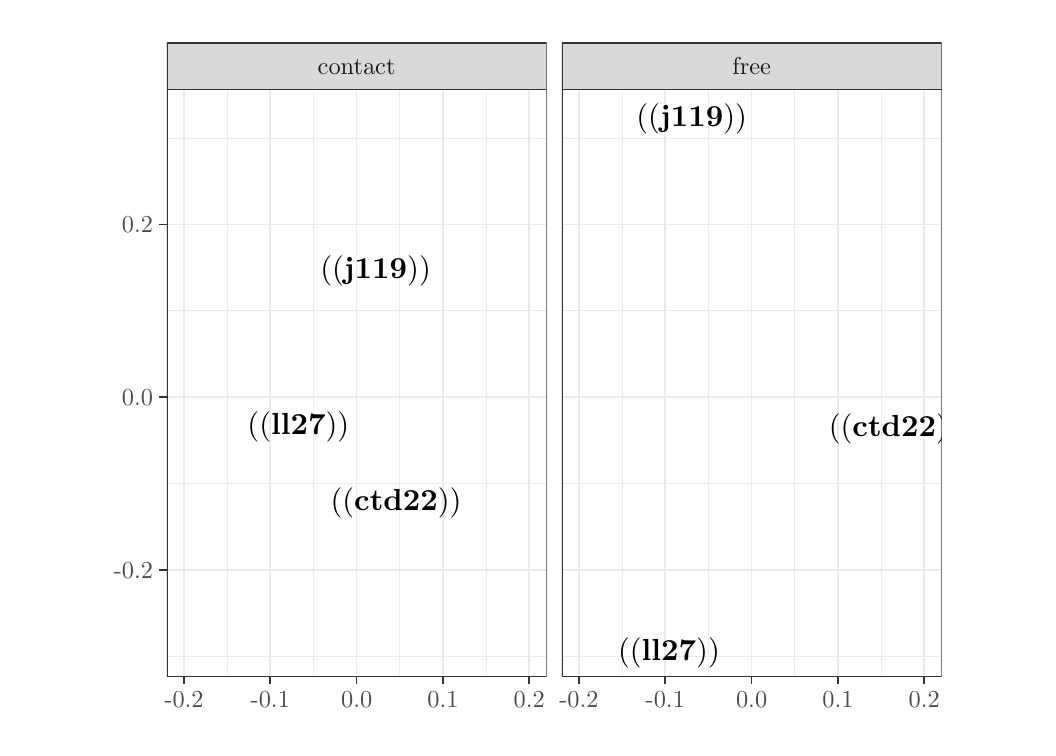
\begin{tikzpicture}[x=1pt,y=1pt]
\definecolor{fillColor}{RGB}{255,255,255}
\path[use as bounding box,fill=fillColor,fill opacity=0.00] (0,0) rectangle (361.35,252.94);
\begin{scope}
\path[clip] ( 25.63,  0.00) rectangle (335.72,252.94);
\definecolor{drawColor}{RGB}{255,255,255}
\definecolor{fillColor}{RGB}{255,255,255}

\path[draw=drawColor,line width= 0.6pt,line join=round,line cap=round,fill=fillColor] ( 25.63,  0.00) rectangle (335.72,252.94);
\end{scope}
\begin{scope}
\path[clip] ( 50.26, 18.45) rectangle (187.49,230.64);
\definecolor{fillColor}{RGB}{255,255,255}

\path[fill=fillColor] ( 50.26, 18.45) rectangle (187.49,230.64);
\definecolor{drawColor}{gray}{0.92}

\path[draw=drawColor,line width= 0.3pt,line join=round] ( 50.26, 25.85) --
	(187.49, 25.85);

\path[draw=drawColor,line width= 0.3pt,line join=round] ( 50.26, 88.23) --
	(187.49, 88.23);

\path[draw=drawColor,line width= 0.3pt,line join=round] ( 50.26,150.61) --
	(187.49,150.61);

\path[draw=drawColor,line width= 0.3pt,line join=round] ( 50.26,212.99) --
	(187.49,212.99);

\path[draw=drawColor,line width= 0.3pt,line join=round] ( 72.09, 18.45) --
	( 72.09,230.64);

\path[draw=drawColor,line width= 0.3pt,line join=round] (103.28, 18.45) --
	(103.28,230.64);

\path[draw=drawColor,line width= 0.3pt,line join=round] (134.47, 18.45) --
	(134.47,230.64);

\path[draw=drawColor,line width= 0.3pt,line join=round] (165.66, 18.45) --
	(165.66,230.64);

\path[draw=drawColor,line width= 0.6pt,line join=round] ( 50.26, 57.04) --
	(187.49, 57.04);

\path[draw=drawColor,line width= 0.6pt,line join=round] ( 50.26,119.42) --
	(187.49,119.42);

\path[draw=drawColor,line width= 0.6pt,line join=round] ( 50.26,181.80) --
	(187.49,181.80);

\path[draw=drawColor,line width= 0.6pt,line join=round] ( 56.50, 18.45) --
	( 56.50,230.64);

\path[draw=drawColor,line width= 0.6pt,line join=round] ( 87.68, 18.45) --
	( 87.68,230.64);

\path[draw=drawColor,line width= 0.6pt,line join=round] (118.87, 18.45) --
	(118.87,230.64);

\path[draw=drawColor,line width= 0.6pt,line join=round] (150.06, 18.45) --
	(150.06,230.64);

\path[draw=drawColor,line width= 0.6pt,line join=round] (181.25, 18.45) --
	(181.25,230.64);
\definecolor{drawColor}{RGB}{0,0,0}

\node[text=drawColor,anchor=base,inner sep=0pt, outer sep=0pt, scale=  1.10] at (125.71,162.42) {\gls{j119}};

\node[text=drawColor,anchor=base,inner sep=0pt, outer sep=0pt, scale=  1.10] at ( 97.80,105.80) {\gls{ll27}};

\node[text=drawColor,anchor=base,inner sep=0pt, outer sep=0pt, scale=  1.10] at (133.11, 78.64) {\gls{ctd22}};
\definecolor{drawColor}{gray}{0.20}

\path[draw=drawColor,line width= 0.6pt,line join=round,line cap=round] ( 50.26, 18.45) rectangle (187.49,230.64);
\end{scope}
\begin{scope}
\path[clip] (192.99, 18.45) rectangle (330.22,230.64);
\definecolor{fillColor}{RGB}{255,255,255}

\path[fill=fillColor] (192.99, 18.45) rectangle (330.22,230.64);
\definecolor{drawColor}{gray}{0.92}

\path[draw=drawColor,line width= 0.3pt,line join=round] (192.99, 25.85) --
	(330.22, 25.85);

\path[draw=drawColor,line width= 0.3pt,line join=round] (192.99, 88.23) --
	(330.22, 88.23);

\path[draw=drawColor,line width= 0.3pt,line join=round] (192.99,150.61) --
	(330.22,150.61);

\path[draw=drawColor,line width= 0.3pt,line join=round] (192.99,212.99) --
	(330.22,212.99);

\path[draw=drawColor,line width= 0.3pt,line join=round] (214.82, 18.45) --
	(214.82,230.64);

\path[draw=drawColor,line width= 0.3pt,line join=round] (246.01, 18.45) --
	(246.01,230.64);

\path[draw=drawColor,line width= 0.3pt,line join=round] (277.20, 18.45) --
	(277.20,230.64);

\path[draw=drawColor,line width= 0.3pt,line join=round] (308.38, 18.45) --
	(308.38,230.64);

\path[draw=drawColor,line width= 0.6pt,line join=round] (192.99, 57.04) --
	(330.22, 57.04);

\path[draw=drawColor,line width= 0.6pt,line join=round] (192.99,119.42) --
	(330.22,119.42);

\path[draw=drawColor,line width= 0.6pt,line join=round] (192.99,181.80) --
	(330.22,181.80);

\path[draw=drawColor,line width= 0.6pt,line join=round] (199.22, 18.45) --
	(199.22,230.64);

\path[draw=drawColor,line width= 0.6pt,line join=round] (230.41, 18.45) --
	(230.41,230.64);

\path[draw=drawColor,line width= 0.6pt,line join=round] (261.60, 18.45) --
	(261.60,230.64);

\path[draw=drawColor,line width= 0.6pt,line join=round] (292.79, 18.45) --
	(292.79,230.64);

\path[draw=drawColor,line width= 0.6pt,line join=round] (323.98, 18.45) --
	(323.98,230.64);
\definecolor{drawColor}{RGB}{0,0,0}

\node[text=drawColor,anchor=base,inner sep=0pt, outer sep=0pt, scale=  1.10] at (239.94,217.19) {\gls{j119}};

\node[text=drawColor,anchor=base,inner sep=0pt, outer sep=0pt, scale=  1.10] at (231.72, 24.30) {\gls{ll27}};

\node[text=drawColor,anchor=base,inner sep=0pt, outer sep=0pt, scale=  1.10] at (313.15,105.36) {\gls{ctd22}};
\definecolor{drawColor}{gray}{0.20}

\path[draw=drawColor,line width= 0.6pt,line join=round,line cap=round] (192.99, 18.45) rectangle (330.22,230.64);
\end{scope}
\begin{scope}
\path[clip] ( 50.26,230.64) rectangle (187.49,247.45);
\definecolor{drawColor}{gray}{0.20}
\definecolor{fillColor}{gray}{0.85}

\path[draw=drawColor,line width= 0.6pt,line join=round,line cap=round,fill=fillColor] ( 50.26,230.64) rectangle (187.49,247.44);
\definecolor{drawColor}{gray}{0.10}

\node[text=drawColor,anchor=base,inner sep=0pt, outer sep=0pt, scale=  0.88] at (118.87,236.01) {contact};
\end{scope}
\begin{scope}
\path[clip] (192.99,230.64) rectangle (330.22,247.45);
\definecolor{drawColor}{gray}{0.20}
\definecolor{fillColor}{gray}{0.85}

\path[draw=drawColor,line width= 0.6pt,line join=round,line cap=round,fill=fillColor] (192.99,230.64) rectangle (330.22,247.44);
\definecolor{drawColor}{gray}{0.10}

\node[text=drawColor,anchor=base,inner sep=0pt, outer sep=0pt, scale=  0.88] at (261.60,236.01) {free};
\end{scope}
\begin{scope}
\path[clip] (  0.00,  0.00) rectangle (361.35,252.94);
\definecolor{drawColor}{gray}{0.20}

\path[draw=drawColor,line width= 0.6pt,line join=round] ( 56.50, 15.70) --
	( 56.50, 18.45);

\path[draw=drawColor,line width= 0.6pt,line join=round] ( 87.68, 15.70) --
	( 87.68, 18.45);

\path[draw=drawColor,line width= 0.6pt,line join=round] (118.87, 15.70) --
	(118.87, 18.45);

\path[draw=drawColor,line width= 0.6pt,line join=round] (150.06, 15.70) --
	(150.06, 18.45);

\path[draw=drawColor,line width= 0.6pt,line join=round] (181.25, 15.70) --
	(181.25, 18.45);
\end{scope}
\begin{scope}
\path[clip] (  0.00,  0.00) rectangle (361.35,252.94);
\definecolor{drawColor}{gray}{0.30}

\node[text=drawColor,anchor=base,inner sep=0pt, outer sep=0pt, scale=  0.88] at ( 56.50,  7.44) {-0.2};

\node[text=drawColor,anchor=base,inner sep=0pt, outer sep=0pt, scale=  0.88] at ( 87.68,  7.44) {-0.1};

\node[text=drawColor,anchor=base,inner sep=0pt, outer sep=0pt, scale=  0.88] at (118.87,  7.44) {0.0};

\node[text=drawColor,anchor=base,inner sep=0pt, outer sep=0pt, scale=  0.88] at (150.06,  7.44) {0.1};

\node[text=drawColor,anchor=base,inner sep=0pt, outer sep=0pt, scale=  0.88] at (181.25,  7.44) {0.2};
\end{scope}
\begin{scope}
\path[clip] (  0.00,  0.00) rectangle (361.35,252.94);
\definecolor{drawColor}{gray}{0.20}

\path[draw=drawColor,line width= 0.6pt,line join=round] (199.22, 15.70) --
	(199.22, 18.45);

\path[draw=drawColor,line width= 0.6pt,line join=round] (230.41, 15.70) --
	(230.41, 18.45);

\path[draw=drawColor,line width= 0.6pt,line join=round] (261.60, 15.70) --
	(261.60, 18.45);

\path[draw=drawColor,line width= 0.6pt,line join=round] (292.79, 15.70) --
	(292.79, 18.45);

\path[draw=drawColor,line width= 0.6pt,line join=round] (323.98, 15.70) --
	(323.98, 18.45);
\end{scope}
\begin{scope}
\path[clip] (  0.00,  0.00) rectangle (361.35,252.94);
\definecolor{drawColor}{gray}{0.30}

\node[text=drawColor,anchor=base,inner sep=0pt, outer sep=0pt, scale=  0.88] at (199.22,  7.44) {-0.2};

\node[text=drawColor,anchor=base,inner sep=0pt, outer sep=0pt, scale=  0.88] at (230.41,  7.44) {-0.1};

\node[text=drawColor,anchor=base,inner sep=0pt, outer sep=0pt, scale=  0.88] at (261.60,  7.44) {0.0};

\node[text=drawColor,anchor=base,inner sep=0pt, outer sep=0pt, scale=  0.88] at (292.79,  7.44) {0.1};

\node[text=drawColor,anchor=base,inner sep=0pt, outer sep=0pt, scale=  0.88] at (323.98,  7.44) {0.2};
\end{scope}
\begin{scope}
\path[clip] (  0.00,  0.00) rectangle (361.35,252.94);
\definecolor{drawColor}{gray}{0.30}

\node[text=drawColor,anchor=base east,inner sep=0pt, outer sep=0pt, scale=  0.88] at ( 45.31, 54.01) {-0.2};

\node[text=drawColor,anchor=base east,inner sep=0pt, outer sep=0pt, scale=  0.88] at ( 45.31,116.39) {0.0};

\node[text=drawColor,anchor=base east,inner sep=0pt, outer sep=0pt, scale=  0.88] at ( 45.31,178.77) {0.2};
\end{scope}
\begin{scope}
\path[clip] (  0.00,  0.00) rectangle (361.35,252.94);
\definecolor{drawColor}{gray}{0.20}

\path[draw=drawColor,line width= 0.6pt,line join=round] ( 47.51, 57.04) --
	( 50.26, 57.04);

\path[draw=drawColor,line width= 0.6pt,line join=round] ( 47.51,119.42) --
	( 50.26,119.42);

\path[draw=drawColor,line width= 0.6pt,line join=round] ( 47.51,181.80) --
	( 50.26,181.80);
\end{scope}
\end{tikzpicture}


\end{knitrout}
Yates' Correction for Continuity:
\[
\chi^2=\frac{(|o_1-e_1|-0.5)^2}{e_1r}+\frac{(|o_2-e_2|-0.5)^2}{e_2r}+...+\frac{(|o_k-e_k|-0.5)^2}{e_kr}
\]
\end{document}
